%----------------------------------------------------------------------------------------
%	PACKAGES AND OTHER DOCUMENT CONFIGURATIONS
%----------------------------------------------------------------------------------------

\documentclass[
12pt,
singlespacing,
headsepline,
]{BachelorThesis} % The class file specifying the document structure

\usepackage[utf8]{inputenc} % Required for inputting international characters
\usepackage[T1]{fontenc} % Output font encoding for international characters
\usepackage{listings}
\usepackage{soul}
\usepackage{adjustbox}
\usepackage{caption}
\usepackage{bm}
\usepackage[titletoc,title]{appendix}
\usepackage[backend=biber,style=authoryear,natbib=true,sorting=none]{biblatex} % Use the bibtex backend with the authoryear citation style (which resembles APA)
\captionsetup[figure]{font=footnotesize,labelfont=footnotesize}
\captionsetup[table]{font=footnotesize,labelfont=footnotesize}
\addbibresource{bibliography.bib} % The filename of the bibliography

\usepackage[autostyle=true]{csquotes} % Required to generate language-dependent quotes in the bibliography

%----------------------------------------------------------------------------------------
%	MARGIN SETTINGS
%----------------------------------------------------------------------------------------

\geometry{
	paper=a4paper, % Change to letterpaper for US letter
	inner=2.5cm, % Inner margin
	outer=3.8cm, % Outer margin
	bindingoffset=.5cm, % Binding offset
	top=1.5cm, % Top margin
	bottom=1.5cm, % Bottom margin
}

%----------------------------------------------------------------------------------------
%	THESIS INFORMATION
%----------------------------------------------------------------------------------------

\thesistitle{Analisi delle prestazioni del\\\emph{Linux Kernel Runtime Guardian}}
\supervisor{Gabriele \textsc{D'Angelo}}
\degree{Ingegneria e Scienze Informatiche}
\author{Simone \textsc{Magnani}}
\university{\href{https://www.unibo.it/it}{Alma Mater Studiorum-Università di Bologna}}
\department{\href{http://www.informatica.unibo.it/it/Dipartimento/sedi-del-dipartimento/unita-organizzativa-di-cesena}{Campus di Cesena}}
\group{Programmazione di Reti}
\faculty{\href{https://corsi.unibo.it/laurea/IngegneriaScienzeInformatiche}{Scuola di Scienze}}

\AtBeginDocument{
\hypersetup{pdftitle=\ttitle} % Set the PDF's title to your title
\hypersetup{pdfauthor=\authorname} % Set the PDF's author to your name
\hypersetup{hidelinks}
}

\begin{document}

\frontmatter % Use roman page numbering style (i, ii, iii, iv...) for the pre-content pages

\nocite{*}

\pagestyle{plain} % Default to the plain heading style until the thesis style is called for the body content

%----------------------------------------------------------------------------------------
%	TITLE PAGE
%----------------------------------------------------------------------------------------

\begin{titlepage}
\begin{center}

\vspace*{.06\textheight}
{\scshape\large \univname\par\deptname\par\facname\par}\vspace{1.5cm} % University name
\textsc{\large Corso di laurea in \degreename}\\[0.5cm] % Thesis type

\HRule \\[0.4cm] % Horizontal line
{\huge \bfseries \ttitle\par}\vspace{0.4cm} % Thesis title
\HRule \\[1.5cm] % Horizontal line
 
\vfill

\large \textit{Relazione finale in}\\[0.3cm] % University requirement text
\groupname\\[2cm] % Research group name and department name

\begin{minipage}[t]{0.4\textwidth}
\begin{flushleft} \large
\emph{Presentata da:}\\
\href{https://www.linkedin.com/in/simone-magnani-564830151/}{\authorname} % Author name

\end{flushleft}
\end{minipage}
\begin{minipage}[t]{0.4\textwidth}
\begin{flushright} \large
\emph{Relatore:} \\
\href{http://www.cs.unibo.it/~gdangelo/}{\supname} % Supervisor name
\end{flushright}
\end{minipage}\\[3cm]
 
\vfill

{\large Sessione II}\\ % Session
{\large Anno Accademico 2017/2018}\\[4cm] % Academic Year
 
\vfill
\end{center}
\end{titlepage}

\cleardoublepage

%----------------------------------------------------------------------------------------
%	QUOTATION PAGE
%----------------------------------------------------------------------------------------

\begin{flushright}
\vspace*{0.2\textheight}
\noindent\enquote{\itshape %Hardware is easy to protect: lock it in a room, chain it to a desk, or buy a spare. Information poses more of a problem. It can exist in more than one place; be transported halfway across the planet in seconds; and be stolen without your knowledge.}\bigbreak
L'hardware è facile da proteggere: lo chiudi in una stanza, lo leghi ad una scrivania, o ne compri uno di ricambio. L'informazione pone molto più di un problema. Può esistere in più di un posto; può essere trasportata attraverso il pianeta in pochi secondi; e può essere rubata senza che tu ne sia a conoscenza.}\bigbreak
\hfill Bruce Schneier, Protect Your Macintosh, 1994
\end{flushright}


%----------------------------------------------------------------------------------------
%	ABSTRACT PAGE
%----------------------------------------------------------------------------------------

\begin{otherlanguage}{english}
\begin{abstract}
\addchaptertocentry{\abstractname}

Gli argomenti d'interesse di questo elaborato sono l'integrità e la sicurezza di un sistema operativo (principalmente Linux). In particolare, viene analizzato il recente software \emph{Linux Kernel Runtime Guardian}, concentrando l'attenzione sulle sue funzionalità ed i controlli effettuati al fine di mantenere il proprio ambiente sicuro.

Prima dell'analisi del sistema, vengono introdotti gli argomenti inerenti per comprendere lo scenario in discussione, quali la sua struttura e gli strumenti in possesso dall'utente per l'interazione. Successivamente vengono presentati sia il software preso in analisi, servendosi della documentazione fornita dall'autore, sia quello progettato ed utilizzato per la misurazione delle performance \emph{SysBench}, interamente sviluppato per calcolare la differenza in termini di tempi di esecuzione di determinate funzionalità in seguito al caricamento di LKRG. Infine, vengono proposti e commentati i risultati sperimentali ottenuti effettuando il test in vari sistemi differenti, al fine di valutarne positivamente o meno l'uso.

Il progetto è OpenSource e si può ottenere clonando il repository nel sito \url{https://bitbucket.org/SimoMagno/sysbench/src/master/}.

\end{abstract}
\end{otherlanguage}

\cleardoublepage

%----------------------------------------------------------------------------------------
%	PREFACE PAGE
%----------------------------------------------------------------------------------------

\begin{preface}
\addchaptertocentry{\prefacename}
La tecnologia è un mondo molto vasto e in continua evoluzione, diventato non solo determinante per lo sviluppo delle società, ma soprattutto invasivo nella quotidianità delle persone. La maggior parte delle azioni svolte nell'arco di una giornata includono l'uso di mezzi tra cui i cellulari, i computer o altri dispositivi con i quali si riesce a reperire o caricare informazioni in rete in breve tempo. Molte persone usano in maniera superficiale tali tecnologie e non sono consapevoli dei numerosi pericoli presenti in rete; non si è abituati ad immaginare che un'informazione digitale che viaggia nel misterioso cyber spazio abbia un ruolo determinante nella nostra vita a pari valore di qualsiasi 'contratto' cartaceo o verbale. 
Talvolta, si sente una frase del tipo: "Ma cosa devo proteggere? E da chi? Io non ho nulla da nascondere".

In un mondo in cui ogni cosa oramai è condivisa in rete da più dispositivi è necessario informarsi sulla sicurezza, ed incentivare lo sviluppo di sistemi di prevenzione affidabili in grado di anticipare una minaccia o, in certi casi, addirittura riparare il danno causato. Bisogna però tenere in considerazione che tali sistemi possano essere non solo costosi economicamente, ma anche in termini di risorse che occupano all'interno del dispositivo. È dunque essenziale durante lo sviluppo di un software tenere in considerazione il grado di soddisfazione del futuro cliente, il quale è influenzato da numerosi fattori come la facilità d'uso e velocità di risposta.

È in questo scenario che nasce \emph{SysBench}, un programma per effettuare un benchmark del sistema in seguito all'utilizzo del modulo di sicurezza \emph{Linux Kernel Runtime Guardian}. Essendo una new entry nel mercato, LKRG non ha ancora ricevuto molte recensioni o analisi delle prestazioni che permettano ad un utente di valutarne seriamente l'uso. Pertanto, viene proposto SysBench come software OpenSource per fornire dati concreti circa le prestazioni di questo modulo. 

\end{preface}
\cleardoublepage

%----------------------------------------------------------------------------------------
%	LIST OF CONTENTS/FIGURES/TABLES PAGES
%----------------------------------------------------------------------------------------

\tableofcontents % Prints the main table of contents
\listoffigures % Prints the list of figures
\listoftables % Prints the list of tables

%----------------------------------------------------------------------------------------
%	THESIS CONTENT - CHAPTERS
%----------------------------------------------------------------------------------------

\mainmatter % Begin numeric (1,2,3...) page numbering

\pagestyle{thesis} % Return the page headers back to the "thesis" style

% Include the chapters of the thesis as separate files from the Chapters folder

\chapter{Introduzione}

\label{Chapter1}

La sicurezza informatica è una tra le varie tematiche più discusse oggigiorno, non solo perchè ha acquisito maggiore importanza l'informazione, ma anche per l'aumento dell'interconnessione dei vari dispositivi. È infatti possibile ottenere o inviare una risorsa da/ad una persona situato dall'altra parte del mondo, condividere in tempo reale i nostri pensieri, esperienze e tant'altro. La cosa più interessante da osservare però è come i \emph{device} o i servizi che utilizziamo quotidianamente proteggano le nostre informazioni, impedendo o meno ad altre persone esterne di accedervi. Nessuno sarebbe contento di sapere che un'altra persona, tramite vari attacchi possibili in rete, è entrata in possesso di dati privati che concernono la propria vita, come la password del proprio conto in banca o la lista dei nostri impegni.
Fortunatamente, per la maggior parte degli sviluppatori è diventato di vitale importanza valorizzare tutto il lato di sicurezza di un sistema prima di fornire un servizio, al fine di garantire all'utente riservatezza ed integrità dei propri dati.

È in questo scenario che nasce \emph{Linux Kernel Runtime Guardian}, un software innovativo con l'obiettivo di mantenere integre e sicure determinate aree del proprio sistema. Prima di parlare della sua struttura e funzionamento, è necessario introdurre gli argomenti teorici inerenti, ovvero le principali componenti di un sistema operativo (nel nostro caso Linux) e le funzionalità che un utente può utilizzare per l'interazione con esso.

%----------------------------------------------------------------------------------------
%	KERNEL
%----------------------------------------------------------------------------------------
\section{Introduzione al kernel}

Molto spesso in informatica i termini \emph{kernel} e \emph{sistema operativo} vengono utilizzati come sinonimi, perchè effettivamente il kernel è il cuore di un sistema operativo, ed ha come obiettivi principali l'interazione con le componenti hardware (hard disk, lettore DVD, etc.) e la fornitura di un ambiente per eseguire le applicazioni utente installate nel sistema.
È inoltre uno tra i primi programmi caricati durante la fase di accensione, senza il quale non sarebbe possibile l'utilizzo delle componenti fisiche.

Il primo kernel Linux è stato sviluppato da Linus Torvald nel 1991, pensato per un'architettura specifica. Negli anni la community di sviluppatori si è ampliata, rendendolo portabile e potente, capace di competere con i più grandi marchi del mercato (Windows, MacOs, etc.). Le sue principali caratteristiche sono:

\begin{itemize}
\item kernel monolitico: è un unico, grande e complesso programma composto da differenti componenti logiche;
\item caricamento dinamico dei moduli: nonostante sia un programma compilato e già in esecuzione nel sistema, offre l'opportunità di caricare/eliminare dinamicamente i moduli (noti come \emph{device driver}), le componenti che lo formano;
\item kernel threading: sono thread (un modo per dividere il programma in più componenti simultanee) del kernel associati ad un programma utente o a qualche funzionalità che Linux utilizza in maniera limitata ed efficiente per eseguire alcuni controlli periodici;
\item supporto per applicazioni multi-thread: supporta come la maggior parte dei sistemi operativi le applicazioni multi-thread;
\item preemptive: può arbitrariamente interrompere l'esecuzione di un task per poi riprenderla in seguito;
\item supporto per sistemi multi-processore: supporta \emph{SMP (symmetric multiprocessing)}, grazie al quale il sistema utilizza più processori, ognuno dei quali gestisce i propri task;
\item Virtual File System: implementando questa tecnologia, è più semplice rispetto agli altri sistemi operativi importare un \emph{file system} (componente logica per il controllo di come e dove le informazioni sono salvate) esterno.
\end{itemize}
L'attributo sul quale vale la pena fare una riflessione ai fini di questo elaborato è il caricamento dinamico dei moduli. Nonostante sia una caratteristica tipica dei sistemi basati su \emph{microkernel}, ovvero sistemi nei quali il kernel è suddiviso in vari servizi nello spazio utente (piuttosto che essere un unico software in esecuzione nello spazio kernel), Linux offre la possibilità di estendere o ridurre le funzionalità del kernel attraverso semplici strumenti.

È sufficiente utilizzare il comando \emph{modprobe} o \emph{insmode} con i privilegi di root (richiesti appunto per operazioni di rilevante importanza) per poter caricare un modulo compilato, al contrario \emph{rmmod} per rimuoverlo. Mentre insmode carica nel kernel il modulo d'interesse senza eseguire controlli di dipendenze tra moduli, modprobe carica anche tutti i moduli richiesti necessari per il corretto funzionamento.
Di seguito, ecco un esempio d'uso di alcuni di questi comandi:

\begin{lstlisting}[
	language=bash,
	basicstyle=\color{black}\ttfamily,
	backgroundcolor=\color{white}]
prova@prova:~$ sudo insmod testModule.ko
[sudo] password for prova:
prova@prova:~$ lsmod | grep testModule
Module
testModule	16384	0
prova@prova:~$ sudo rmmod testModule.ko
prova@prova:~$ lsmod | grep testModule
prova@prova:~$ 
\end{lstlisting}
È possibile osservare come una volta caricato con successo, il modulo appaia nella lista di quelli attualmente in esecuzione nel kernel (comando \emph{lsmod}). Nelle prossime sezioni verrà spiegato come un utente si può interfacciare con un modulo, leggendo l'output che esso produce o modificando determinati parametri.

\subsection{Architettura di un modulo}
Il linguaggio di programmazione utilizzato per creare un modulo è il C, con qualche differenza rispetto ai classici programmi che si è abituati a scrivere. Infatti, mentre tutti i programmi utente scritti in C richiedono che ci sia una funzione \emph{main}, nel sorgente del modulo bisogna specificare due funzioni: una di inizializzazione e una di uscita.
A scelta dello sviluppatore ma altamente consigliato per creare una buona documentazione, possono essere indicate informazioni quali la licenza, l'autore, la descrizione e una versione del modulo. Tali attributi possono essere consultati una volta compilato il modulo con il comando \emph{modinfo module\_name}.
Una volta compilato tramite un apposito \emph{makefile}, ovvero un file contenente una serie di direttive per la compilazione, si ottiene la versione \emph{.ko} del sorgente in formato ELF (Executable and Linkable Format), la quale può essere caricata con i metodi illustrati.

Osserviamo un esempio di un modulo per avere un'idea più precisa:

\begin{lstlisting}[
	language=C,
  	keywordstyle=\bfseries\color{green!40!black},
  	commentstyle=\itshape\color{purple!40!black},
  	identifierstyle=\color{blue},
  	stringstyle=\color{orange},
    basicstyle=\scriptsize\ttfamily,
    breaklines=true]
#include <linux/module.h>
#include <linux/kernel.h>
#include <linux/init.h>

static int __init hello_init(void)
{
	printk(KERN_INFO "Hello world!\n");
	return 0;
}

static void __exit hello_exit(void)
{
	printk(KERN_INFO "Goodbye World!\n");	
}

module_init(hello_init);
module_exit(hello_exit);

MODULE_LICENSE("GPL");
MODULE_AUTHOR("Simone Magnani");
MODULE_DESCRIPTION("Hello world module!");
MODULE_VERSION("0.1");
\end{lstlisting}

Tralasciando le informazioni autoesplicative finali, in tutti i moduli sono richiamate le macro \emph{module\_init} e \emph{module\_exit} alle quali vengono passate come parametri le corrispettive funzioni di inizializzazione e terminazione. Fino alla versione 2.4 del kernel, era sufficiente dichiarare tale funzioni con i nomi \emph{init\_module} e \emph{cleanup\_module}, ma per comodità di progettazione si è scelto di introdurre le macro. Il modulo una volta caricato produce come output "Hello World", mentre "Goodbye World" è il messaggio stampato durante la fase di rimozione.

È possibile trovarsi in una situazione in cui un modulo 'A' debba utilizzare delle funzioni che, per scelta progettuale o stilistica, sono implementate nel modulo 'B'. Tutto quello che serve fare è creare un \emph{header file} nel quale è dichiarato il prototipo della funzione, includerlo nel modulo 'A' tramite la direttiva \emph{include} e aggiungere alla fine dell'implementazione della funzione nel modulo 'B' la riga \emph{EXPORT\_SYMBOL(function\_name)}. Infine, è strettamente necessario che il modulo 'B' che è una sorta di 'fornitore' della specifica sia caricato prima di 'A', altrimenti la risoluzione dei simboli fallirebbe.
Per quello che ci concerne, queste sono le poche informazioni indispensabili che servono per comprendere come funziona il kernel, nel caso volessimo consultare il sorgente del software \emph{LKRG} o scrivere un proprio modulo di utility.

\subsection{Comunicazione utente-kernel}
In questa sezione vengono trattati i vari metodi di comunicazione tra lo spazio utente e kernel, ponendo maggiore importanza nell'utilizzo del \emph{Virtual File System (VFS)} e delle \emph{sysctl}, i due metodi più comunemente utilizzati. Quest'ultimo in particolare è il principio di base su cui si basa l'interazione tra l'utente e il modulo LKRG, con il quale è possibile modificare determinati parametri del kernel.

Vi sono in linux diversi modi per interagire con il kernel, tra cui:

\begin{enumerate}
\item Virtual File System (Procfs, Sysfs, Configfs, Debugfs, Character Devices)
\item Socket based mechanism (Udp sockets, Netlink sockets)
\item Ioctl (input-output control)
\item System call
\item Kernel signaling
\item Upcall
\item Mmap
\end{enumerate}

Linux implementa il concetto di virtual file system, grazie al quale l'utente può accedere a diversi tipi di file system in maniera uniforme; inoltre a seconda dell'utilizzo è possibile montarli (renderli accessibili) liberamente senza dover rispettare alcun vincolo.
Diversi possiedono una propria interfaccia grazie alla quale è più semplice interagire, tra cui ricordiamo:

\begin{itemize}
\item /proc
\item /sys
\item /dev
\item /sys/kernel/config (a volte anche solo /config)
\item /sys/kernel/debug
\end{itemize}

Inizialmente progettato per esportare tutte le informazioni riguardanti i processi, come lo stato corrente e i file descriptor aperti, \emph{/proc} è ampliamente utilizzato per fornire dati circa:

\begin{itemize}
\item il sistema in esecuzione (CPU, memoria, interrupt, etc.);
\item i device 'ide', 'scsi' e 'tty\'s';
\item la rete, come la tabella \emph{ARP} (Address resolution Protocol), la lista delle socket utilizzate o qualche statistica.
\end{itemize}

In aggiunta, al suo interno vi è un'importante cartella denominata \emph{/proc/sys}, la quale permette di configurare numerosi parametri del sistema, ognuno rappresentato da un singolo file. Tutte le sotto cartelle e i file interni non sono implementati secondo l'interfaccia \emph{procfs}, bensì rispondono ad un meccanismo del kernel appositamente costruito chiamato \emph{sysctl}.

A differenza della filosofia dei file system, secondo la quale il kernel può modificare un file ma l'utente rimane inconscio di questa modifica fino alla prossima apertura, tramite l'utilizzo delle \emph{socket} il kernel può inviare notifiche ad un'applicazione utente in ascolto in qualsiasi momento. Vi sono 3 diverse famiglie da poter utilizzare:

\begin{itemize}
\item AF\_INET: progettate per la comunicazione in rete, è possibile utilizzare socket \emph{UDP (User Datagram Protocol)}, nonostante vi possa essere più sovraccarico di messaggi.
\item AF\_PACKET: permette all'utente di definire gli headers dei pacchetti.
\item AF\_NETLINK: specialmente progettate per la comunicazione tra utente e kernel.
\end{itemize}

Tra le varie chiamate di sistema che analizzeremo nella prossima sezione, esiste la funzione \emph{ioctl()} grazie alla quale è possibile manipolare i parametri di determinati device. È implementata come un'unica funzione, la quale effettua la multiplazione dei comandi al fine che vengano richiesti i device opportuni. Il \emph{multiplexing} si basa sul \emph{file descriptor}, un puntatore astratto a quella specifica risorsa o canale, e il numero del comando da eseguire su quel preciso device.

L'invio di segnali da parte del kernel è un approcio leggermente diverso dai classici, dato che solo il kernel può inviare segnali allo spazio utente e non vice versa. Inoltre il quantitativo di dati trasportati dai segnali è molto limitato. Esistono due tipi diversi di API nello \emph{user space}: le 'normali', le quali non trasportano dati, e le 'realtime' che trasportano fino ad un massimo di 32 bit.
Affinchè il segnale sia ricevuto, nello spazio utente è necessario registrare un'apposita funzione con il compito di essere notificata; tale funzione sarà richiamata ogni volta che il kernel invierà un segnale di quel tipo.

Grazie all'uso delle \emph{Upcall}, un modulo del kernel può invocare l'esecuzione di un programma utente nell'apposito spazio, configurando gli appositi parametri e variabili d'ambiente. Possiamo definire tale procedimento 'ad hoc', in quanto un qualsiasi utente solitamente non programma un apposito modulo per ogni programma che vuole eseguire, ma può risultare molto utile come tecnica nel caso dovesse utilizzare un programma specifico.

Infine, l'unico modo per trasferire grandi quantitativi di dati tra l'utente e il kernel senza effettuarne una copia, è il \emph{memory mapping} ('mmap', mappatura della memoria). Sostanzialmente, si definisce un'area della memoria accessibile sia al kernel che all'utente, nella quale ogni attore può scrivere o leggere i dati contenuti. La differenza con le tecniche mostrate fino ad ora, risiede nella notificazione dei cambiamenti: con mmap, quando un attore scrive dei dati nella porzione condivisa, l'altro non è a conoscenza di tali cambiamenti fino a quando non ne effettua la lettura. Nel caso non vi fossero delle politiche di lettura/scrittura, se i due attori scrivessero nel buffer senza prima 'consumare' l'informazione comunicata dall'altro, vi è una perdita di dati.

\subsection{Esempi di comunicazione}

Vengono proposti i due esempi di comunicazione più classici ampiamente utilizzati nella programmazione del kernel.
Il primo metodo sfrutta il famigerato file system /proc, creando una entry del nostro modulo non appena esso viene caricato, assegnando le funzioni di lettura e scrittura che dichiariamo; in tale modo è possibile scrivere all'interno del file e leggerne il contenuto secondo le nostre politiche, implementate nelle apposite funzioni \emph{write\_proc()} e \emph{read\_proc()}.
Questo esempio è stato testato nella versione 4.15.0.33-generic del kernel Linux.

\begin{lstlisting}[
	language=C,
  	keywordstyle=\bfseries\color{green!40!black},
  	commentstyle=\itshape\color{purple!40!black},
  	identifierstyle=\color{blue},
  	stringstyle=\color{orange},
    basicstyle=\scriptsize\ttfamily,
    breaklines=true]
#include <linux/module.h>
#include <linux/kernel.h>
#include <linux/proc_fs.h>
#include <linux/sched.h>
#include <linux/uaccess.h>
#include <linux/slab.h>
#define MSG_SIZE (512)

static char *msg;
static int len,tmp;

ssize_t write_proc(struct file *filp, const char *buf, size_t count, loff_t *offp)
{
    unsigned long actual_len = count < MSG_SIZE - 1 ? count : MSG_SIZE - 1;
    copy_from_user(msg, buf, actual_len);
    len = count;
    tmp = len;
    return len;
}

ssize_t read_proc(struct file *filp, char *buf, size_t count, loff_t *offp)
{
    if(count > tmp) 
        count = tmp;
    tmp = tmp - count;
    copy_to_user(buf, msg, count);
    if(count == 0)
        tmp = len;
    return count;
}

struct file_operations proc_fops =
{
write:
    write_proc,
read:
    read_proc
};

static int __init proc_init(void)
{
    if ((msg = kmalloc(MSG_SIZE, GFP_KERNEL)) == NULL)
        return -ENOMEM;
    proc_create("myProc", 0, NULL, &proc_fops);
    return 0;
}

static void __exit proc_exit(void)
{
    remove_proc_entry("myProc", NULL);
    kfree(msg);
}

MODULE_LICENSE("GPL");
module_init(proc_init);
module_exit(proc_exit);
\end{lstlisting}

Si è dichiarato un buffer denominato \emph{msg} il quale ha il compito di tenere in memoria il contenuto della nostra entry \emph{myEntry}. Nella struttura \emph{file\_operations}, sono state agganciate le nostre rispettive funzioni di write e read, le quali non fanno altro che copiare il messaggio utente in msg nel primo caso,  viceversa nel secondo.
È molto importante eliminare la entry e liberare la memoria allocata per il nostro buffer quando il modulo viene rimosso, onde evitare errori o sprechi inutili di memoria.
Una volta caricato nel kernel, per interagire con il nuovo file /proc/myEntry è sufficiente utilizzare dei semplici comandi \emph{cat} e \emph{echo} come di seguito:

\begin{lstlisting}[
	language=bash,
	basicstyle=\color{black}\ttfamily,
	backgroundcolor=\color{white}]
prova@prova:~$ sudo insmod proc_entry.ko
[sudo] password for prova:
prova@prova:~$ lsmod | grep proc_entry
Module
proc_entry	16384	0
prova@prova:~$ echo "Ciao Mondo" > /proc/myEntry
prova@prova:~$ cat /proc/myEntry
Ciao Mondo
prova@prova:~$ 
\end{lstlisting}

Il secondo esempio proposto sfrutta la funzionalità \emph{sysctl} del kernel, con la quale è possibile modificare determinati parametri a runtime sfruttando la directory /sys all'interno del file system /proc. 

\begin{lstlisting}[
	language=C,
  	keywordstyle=\bfseries\color{green!40!black},
  	commentstyle=\itshape\color{purple!40!black},
  	identifierstyle=\color{blue},
  	stringstyle=\color{orange},
    basicstyle=\scriptsize\ttfamily,
    breaklines=true]
#include <linux/module.h>
#include <linux/kernel.h>
#include <linux/sysctl.h>

int my_var = 0;

static struct ctl_table_header *my_header;

static struct ctl_table my_value[] =
{
    {
        .procname       = "my_value",
        .data           = &my_var,
        .maxlen         = sizeof(int),
        .mode           = 0600,
        .proc_handler   = proc_dointvec_minmax,
    },
    {}
};

static struct ctl_table my_directory[] =
{
    {
        .procname    = "example",
        .mode        = 0600,
        .child       = my_value,
    },
    { }
};

static int __init myInit(void)
{
    /* register the above sysctl */
    my_header = register_sysctl_table(my_directory);
    if (!my_header)
        return -EFAULT;
    return 0;
}

static void __exit myExit(void)
{
    unregister_sysctl_table(my_header);
}

MODULE_LICENSE("GPL");
module_init(myInit);
module_exit(myExit);
\end{lstlisting}

Il modulo crea una propria directory (all'interno di /proc/sys/) chiamata `example` con all'interno l'attributo \emph{my\_value}, al cui cambiamento viene risettato il valore della variabile \emph{my\_var} (il nostro "parametro" del kernel). Configurata la directory, viene registrata all'interno della tabella delle sysctl, e viene ritornato l'header a questa struttura, il quale serve non solo per verificare se l'operazione è andata a buon fine, ma anche per rimuovere l'entry dalla tabella delle sysctl durante la rimozione del modulo.
Di seguito viene mostrato un'esempio d'uso del comando \emph{sysctl} con il nostro parametro registrato:

\begin{lstlisting}[
	language=bash,
	basicstyle=\color{black}\ttfamily,
	backgroundcolor=\color{white}]
prova@prova:~$ sudo insmod sysctl.ko
[sudo] password for prova:
prova@prova:~$ lsmod | grep sysctl
Module
sysctl	16384	0
prova@prova:~$ sysctl -a | grep my\_value
example.my_value = 0
prova@prova:~$ sysctl example.my\_value=100
example.my_value = 100
prova@prova:~$ sysctl -a | grep my\_value
example.my_value = 100
\end{lstlisting}

Un ultimo dettaglio su questo strumento: l'entry aggiunta al file system /proc viene rimossa al successivo riavvio della macchina, a meno che non vengano aggiunte queste preferenze al file \emph{/etc/sysctl.conf}.

%----------------------------------------------------------------------------------------
%	ARCHITECTURE
%----------------------------------------------------------------------------------------
\section{Architettura di un processore}

L'idea di porre dei livelli gerarchici di protezione processore e della memoria (cosiddetti \emph{ring}), è stata per la prima volta introdotta nel computer \emph{GE 645} nel 1965. Questa innovazione è stata molto apprezzata e rivisitata dalla maggior parte dei concorrenti nel mondo informatico, ed è persino utilizzata tutt'ora, seppure con qualche modifica.\\\\
L'idea consiste nell'inserire dei controlli riguardanti l'accesso al processore, per proteggere il sistema in base alla tipologia di operazione che deve svolgere. Tali controlli possono essere implementati in 3 modi:

\begin{itemize}
\item hardware(HW): i livelli di privilegi sono implementati in microcodice HW per il controllo degli accessi;
\item software(SW): il meccanisco di controllo è interamente a livello SW;
\item hardware + software (ibridi): componenti di entrambe le nature collaborano nella gestione dei ring.
\end{itemize}

Generalmente i sistemi con i controlli ibridi sono ottenuti combinando componenti progettate appositamente per tale funzionamento. Supponiamo di avere un computer con il processore strutturato per la cooperazione con un sistema operativo che, diversamente, implementa i controlli solamente a livello software. Cosa succede? Sicuramente potremmo affermare di non avere una gestione dei livelli sia software che hardware, in quanto nel sistema non è integrata questa funzionalità.

Il numero di ring può variare, ma generalmente quelli più interessanti da sapere che sono presenti in tutte le implementazioni sono due: livello 0 (kernel mode) e livello utente (user mode). Mentre il livello 0 è utilizzato dal sistema operativo e rappresenta la massima affidabilità, il livello utente è il livello meno privilegiato, dal quale il sistema si aspetta che le operazioni possano essere malevole.

\begin{figure}[!ht]
\centering
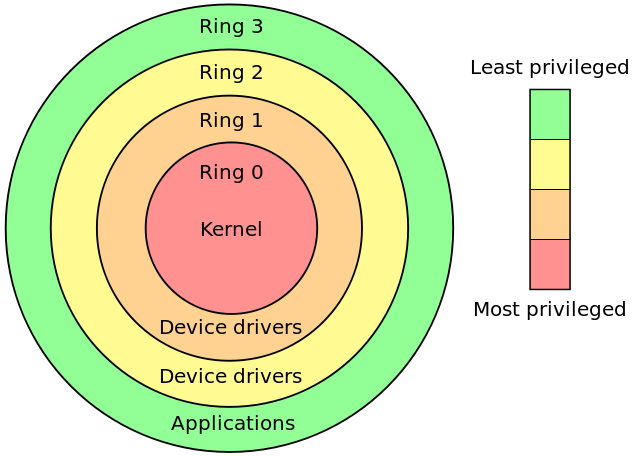
\includegraphics[scale=0.3]{Figures/RingCpu}
\caption[Ring nei processori della famiglia x86]{Ring nei processori della famiglia x86.\\Fonte: \href{https://en.wikipedia.org/wiki/Protection_ring}{https://en.wikipedia.org}}
\label{fig:RingCpu}
\end{figure}

Si può notare in \autoref{fig:RingCpu} che tra i due livelli appena discussi ve ne sono altri due utilizzati dai \emph{device drivers}, ossia da quei programmi che controllano e gestiscono determinati dispositivi fisici o virtuali collegati al calcolatore. Un esempio molto comune è l'installazione della propria stampante a casa: quando viene richiesto di scaricare/aggiornare i driver, si tratta di queste risorse che si interfacciano con il dispositivo fisico.

\subsection{User/Kernel spaces}

La memoria di un calcolatore è suddivisa in due importanti aree: \emph{user space} (spazio utente) e \emph{kernel space} (spazio kernel).

Con il termine user space si fa riferimento a tutto il codice eseguito al di fuori del kernel del sistema operativo. Ogni processo eseguito in questo spazio ha una propria memoria virtuale e non può comunicare, a meno che non venga esplicitato attraverso varie tecniche di programmazione, con gli altri processi. È importante sottolineare che un processo nello spazio utente non ha completo accesso alle risorse di sistema; l'utilizzo di tali risorse è garantito dalle varie \emph{API (Application Programming Interface)} messe a disposizione dal sistema.

Il kernel space ha la proprietà di eseguire il codice a livello 0, tipicamente definita esecuzione in kernel mode. In tale modalità, i processi godono del completo accesso all'hardware e alle risorse, in quanto sono considerati affidabili.

\begin{figure}[!ht]
\centering
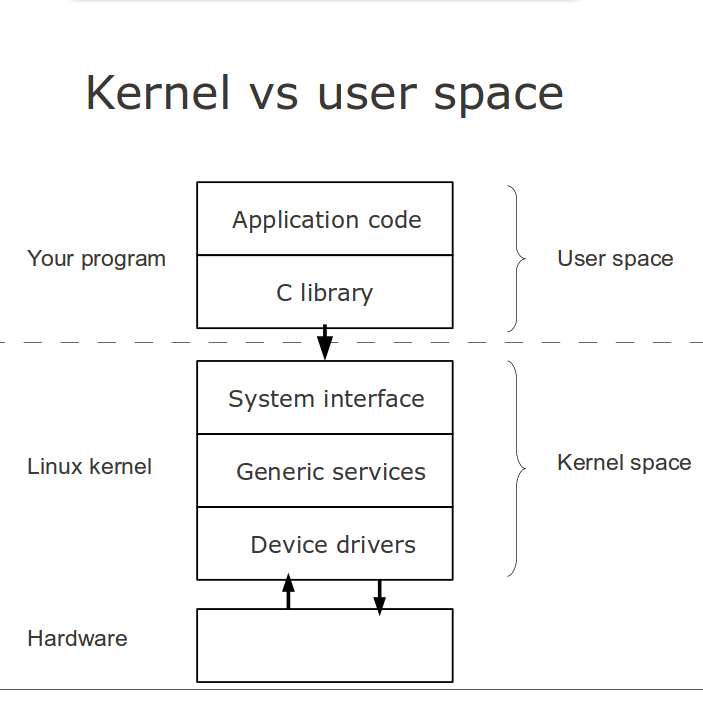
\includegraphics[scale=0.3]{Figures/Spaces}
\caption[Kernel space e User space]{Kernel space e User space.\\ Fonte: \href{https://3.bp.blogspot.com/-s-8vrCL_OPg/V33EJafdJTI/AAAAAAAAPcY/rKlsSv2ay-IYRHLoZdKS07YIgPVS9JX9QCLcB/s1600/Screenshot+from+2016-07-07_08-18-32.png}{https://3.bp.blogspot.com}}
\label{fig:KUSpace}
\end{figure}

La \autoref{fig:KUSpace} rappresenta i due diversi livelli di spazio e come si interfacciano con l'hardware.
Supponiamo di dover lanciare un programma C che esegue una semplice operazione di scrittura su disco (ad esempio salvataggio di un file) per poi terminare. Come discusso poco fa, l'esecuzione del nostro programma avviene nello user space, ovvero lo spazio dove l'accesso diretto all'hardware non è permesso onde evitare danni alle risorse. L'eseguibile dovrà pertanto effettuare una richiesta (detta anche segnalazione) al sistema grazie alla quale avviene la scrittura su disco. Come è possibile che sia avvenuta l'operazione nonostante il mio programma è eseguito nello spazio utente in modalità utente?
Quando il programma ha inviato la segnalazione al sistema, la \emph{CPU (Control Processor Unit)} ha effettuato un'operazione di scambio molto importante tra il ring 0 ed il ring utente grazie alla quale in nostro programma riesce a terminare con successo: il \emph{mode switch}.

\subsection{CPU mode switch}

Talvola il termine \emph{mode switch} viene confuso con \emph{context switch}, sebbene siano due cose concettualmente diverse. Mentre con il secondo si indica il passaggio effettuato dallo scheduler della CPU da un processo o thread ad un altro, il mode switch è il cambio di modalità di esecuzione delle istruzioni all'interno dello stesso processo. Quando il programma utente effettua una segnalazione di sistema per richiedere l'utilizzo di determinato hardware, all'interno della CPU avviene un cambio di modalità, passando dall'esecuzione in modalità utente alla modalità kernel. Avendo ora i privilegi necessari, è possibile soddisfare la richiesta e, una volta terminata, verrà effettuato un ulteriore passaggio per ritornare alla modalità utente.

Il mode switch e il context switch a seconda di come sono implementati possono avere un costo di esecuzione in termine di tempo molto variabile. Per questo si cerca di progettare il sistema operativo in maniera da effettuare il minor numero di passaggi che, nonostante avvengano in tempi pari all'ordine del nanometro, sono impercettibili all'essere umano ma non trascurabili per il processore.
Uno dei vantaggi da sempre riconosciuto a Linux è proprio quello di aver un costo estremamente basso per effettuare tali operazioni.

\section{Le system call}

Fino ad ora si è parlato di interfacce per segnalare al sistema la richiesta di un'istruzione privilegiata senza spiegare altro. Queste funzioni sono conosciute con il nome di \emph{system call (chiamate di sistema)} e sono presenti in ogni sistema operativo, sebbene in maniera differente. Infatti tali funzioni non sono universali per problemi di incompatibilità sia hardware che software; ogni sistema operativo ne possiede delle proprie, le quali hanno comunque come unico obiettivo l'interazione del programma con il sistema e i device che ne fanno parte.

\begin{figure}[!ht]
\centering
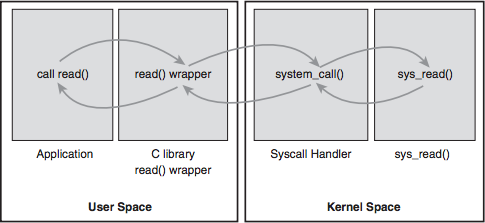
\includegraphics[scale=0.7]{Figures/Syscall}
\caption[Esempio di system call read()]{Esempio di system call read().\\ Fonte: \href{https://www.quora.com/How-does-System-Call-return-data-back-to-user-space-in-Linux-Kernel}{https://www.quora.com}}
\label{fig:Syscall}
\end{figure}

La \autoref{fig:Syscall} mostra un esempio di chiamata della system call \emph{read()}: tra la chiamata a funzione nella nostra applicazione e la vera chiamata di sistema, si noti come è presente un \emph{call wrapper}. Un wrapper consiste in un \emph{layer} di codice con il compito di tradurre in un'interfaccia compatibile il codice di libreria; è sostanzialmente un API grazie alla quale non vi è bisogno di reimplementare del codice, ma si utilizza l'interfaccia che tale prodotto mette a disposizione.
La chiamata \emph{read()} è in realtà un'invocazione del wrapper presente nella libreria standard del linguaggio C (\emph{glibc}), il quale ha il compito a sua volta di richiamare la vera e propria system call.
Una volta invocata ed avvenuto il \emph{mode switch} in quanto deve essere eseguito del codice kernel, un \emph{handler} (intercettatore) inoltra la chiamata ad un livello inferiore, oltre al quale avviene l'operazione vera e propria sul device (fisico o virtuale) d'interesse. Alla fine dell'operazione, la CPU ritorna in modalità utente ed il controllo viene restituito al programma.

Una lista completa di tutte le system call con documentazione può essere trovata nel sito \url{http://man7.org/linux/man-pages/man2/}.

\subsection{Esempi di strumenti utili}
In questa sezione vengono mostrati brevemente degli strumenti da riga di comando molto utili per la fase di debugging del nostro programma, nel caso fossimo interessati a comprenderne il funzionamento a più basso livello.
Supponiamo di avere il nostro programma C come segue:

\begin{lstlisting}[
  	language=C,
  	keywordstyle=\bfseries\color{green!40!black},
  	commentstyle=\itshape\color{purple!40!black},
  	identifierstyle=\color{blue},
  	stringstyle=\color{orange},
    basicstyle=\scriptsize\ttfamily,
    breaklines=true,
    escapechar=\!]
#include <fcntl.h>

int main(void)
{
	int fd = open("foo.txt", O\_RDONLY);
	if(fd > 0) close(fd);
	return 0;
}
\end{lstlisting}

Nella funzione main viene dichiarato un intero all'interno del quale verrà salvato il file descriptor di \emph{foo.txt} nel caso il file esista, altrimenti -1. Se l'apertura del file è avvenuta con successo, si prosegue con la semplice chiusura.
Le funzioni \emph{open()} e \emph{close()} sono delle chiamate di sistema, le quali comunicano al kernel di eseguire tali operazioni privilegiate nell'hardware.
Grazie al comando \emph{strace} è possibile visualizzare tutte le system call effettuate dal nosto programma. Lanciando il comando \emph{strace ./myprogram} dove \emph{myprogram} è l'eseguibile ottenuto in seguito alla compilazione, si ottiene un output simile:

\begin{lstlisting}[
  	language=C,
  	basicstyle=\scriptsize\ttfamily\color{black},
    backgroundcolor=\color{white},
    breaklines=true,
  	escapeinside={(*@}{@*)}]
prova@prova:~$ strace ./myprogram

execve("./myprogram", ["./myprogram"], [/* 70 vars */]) = 0
brk(0)                                  = 0x22c3000
access("/etc/ld.so.nohwcap", F_OK)      = -1 ENOENT (No such file or directory)
mmap(NULL, 8192, PROT_READ|PROT_WRITE, MAP_PRIVATE|MAP_ANONYMOUS, -1, 0) = 0x7f8feb036000
access("/etc/ld.so.preload", R_OK)      = -1 ENOENT (No such file or directory)
open("/etc/ld.so.cache", O_RDONLY|O_CLOEXEC) = 3
fstat(3, {st_mode=S_IFREG|0644, st_size=79132, ...}) = 0
mmap(NULL, 79132, PROT_READ, MAP_PRIVATE, 3, 0) = 0x7f8feb022000
close(3)                                = 0
access("/etc/ld.so.nohwcap", F_OK)      = -1 ENOENT (No such file or directory)
open("/lib/x86_64-linux-gnu/libc.so.6", O_RDONLY|O_CLOEXEC) = 3
read(3, "\177ELF\2\1\1\0\0\0\0\0\0\0\0\0\3\0>\0\1\0\0\0P \2\0\0\0\0\0"..., 832) = 832
fstat(3, {st_mode=S_IFREG|0755, st_size=1840928, ...}) = 0
mmap(NULL, 3949248, PROT_READ|PROT_EXEC, MAP_PRIVATE|MAP_DENYWRITE, 3, 0) = 0x7f8feaa51000
mprotect(0x7f8feac0b000, 2097152, PROT_NONE) = 0
mmap(0x7f8feae0b000, 24576, PROT_READ|PROT_WRITE, MAP_PRIVATE|MAP_FIXED|MAP_DENYWRITE, 3, 0x1ba000) = 0x7f8feae0b000
mmap(0x7f8feae11000, 17088, PROT_READ|PROT_WRITE, MAP_PRIVATE|MAP_FIXED|MAP_ANONYMOUS, -1, 0) = 0x7f8feae11000
close(3)                                = 0
mmap(NULL, 4096, PROT_READ|PROT_WRITE, MAP_PRIVATE|MAP_ANONYMOUS, -1, 0) = 0x7f8feb021000
mmap(NULL, 8192, PROT_READ|PROT_WRITE, MAP_PRIVATE|MAP_ANONYMOUS, -1, 0) = 0x7f8feb01f000
arch_prctl(ARCH_SET_FS, 0x7f8feb01f740) = 0
mprotect(0x7f8feae0b000, 16384, PROT_READ) = 0
mprotect(0x600000, 4096, PROT_READ)     = 0
mprotect(0x7f8feb038000, 4096, PROT_READ) = 0
munmap(0x7f8feb022000, 79132)           = 0
(*@\hl{open("foo.txt", O\_RDONLY)               = 3}@*)
(*@\hl{close(3)                                = 0}@*)
exit_group(0)                           = ?
+++ exited with 0 +++
\end{lstlisting}

Le due righe evidenziate corrispondono esattamente alle due system call richiamate nel programma C, quindi possiamo affermare che quando viene effettuata l'apertura di un file, una scrittura, una lettura o operazioni simili avviene effettivamente la chiamata di una system call con tutto il procedimento di mode switch presentato nella precedente sezione. L'esempio proposto è piuttosto banale e l'uso del comando strace in una situazione del genere è pressochè inutile, ma si immagini in un software molto più complesso quanto possa essere utile analizzare il numero di system call effettuate, al fine di stimare e/o ridurre il tempo di esecuzione in kernel mode.

Un altro comando proposto è \emph{objdump} (esistono comandi molto più potenti e interattivi, come \emph{radare} o \emph{gdb}, ma meno semplici da utilizzare), il quale permette di disassemblare l'eseguibile ed ottenere il codice in linguaggio Assembly corrispondente.
Scrivendo in un terminale \emph{objdump -d myprogram}, si comunica al tool di effettuare il disassemblaggio dell'eseguibile \emph{myprogram}. Eliminando un po' di output non interessante e concentrandoci sulla funzione \emph{main} si ottiene:

\begin{lstlisting}[
	language={[x86masm]Assembler},
	basicstyle=\scriptsize\ttfamily\color{black},
  backgroundcolor=\color{white},
	escapechar=\!]
prova@prova:~$ objdump -d myprogram
...
000000000040057d <main>:
  40057d:	55                   	push   %rbp
  40057e:	48 89 e5             	mov    %rsp,%rbp
  400581:	48 83 ec 10          	sub    $0x10,%rsp
  400585:	be 00 00 00 00       	mov    $0x0,%esi
  40058a:	bf 44 06 40 00       	mov    $0x400644,%edi
  40058f:	b8 00 00 00 00       	mov    $0x0,%eax
  400594:	e8 e7 fe ff ff       	   !\hl{callq  400480 <open@plt>}!
  400599:	89 45 fc             	mov    %eax,-0x4(%rbp)
  40059c:	83 7d fc 00          	cmpl   $0x0,-0x4(%rbp)
  4005a0:	7e 0f                	jle    4005b1 <main+0x34>
  4005a2:	8b 45 fc             	mov    -0x4(%rbp),%eax
  4005a5:	89 c7                	mov    %eax,%edi
  4005a7:	b8 00 00 00 00       	mov    $0x0,%eax
  4005ac:	e8 9f fe ff ff       	   !\hl{callq  400450 <close@plt>}!
  4005b1:	b8 00 00 00 00       	mov    $0x0,%eax
  4005b6:	c9                   	leaveq 
  4005b7:	c3                   	retq   
  4005b8:	0f 1f 84 00 00 00 00 	nopl   0x0(%rax,%rax,1)
  4005bf:	00 
\end{lstlisting}

Come nell'output precedente, sono riportate in evidenza le due chiamate di sistema \emph{open()} e \emph{close()} con le relative operazione intermedie di caricamento parametri nei registri della CPU e pulizia di registri dove salvare l'output. Per chi volesse comprendere il significato di \emph{@plt}, è possibile trovato una soddisfacente spiegazione nel seguente sito \url{https://www.technovelty.org/linux/plt-and-got-the-key-to-code-sharing-and-dynamic-libraries.html}.
Le system call e il codice assembly variano a seconda dell'architettura e del sistema operativo, quindi è molto probabile che lanciando i comandi proposti non si ottengano gli stessi risultati.

\chapter{Il progetto \emph{Linux Runtime Guardian Kernel}}

\label{Chapter2}

\begin{figure}[!ht]
\centering

\includegraphics[scale=0.15]{Figures/Lkrg}
\caption[Logo del software Linux Runtime Guardian Kernel]{Logo del software Linux Runtime Guardian Kernel\\Fonte: \href{https://openwall.info/wiki/p_lkrg/Main}{\url{https://openwall.info}}}
\label{fig:Lkrg}
\end{figure}


LKRG è un software gratuito Open Source sviluppato da Adam 'pi3' Zabrocki, un dipendente della Microsoft amante della sicurezza informatica. Si può ottenere in 3 forme differenti: la versione a pagamento, quella 'light' oppure quella sperimentale, la quale differisce per le funzionalità introdotte, nonostante la possibile presenza di bug.

Come sottolinea nella pagina di documentazione l'autore, LKRG è ancora lontano dall'essere una soluzione perfetta per la sicurezza del kernel (può essere bypassato), ma un corretto uso soprattutto se installato in un sistema stabile e non già compromesso potrebbe migliorarne l'integrità e la sicurezza. Infatti gli obiettivi di questo modulo sono:

\begin{itemize}
\item prevenire le modifiche non supportate al kernel, inserendo delle regole da rispettare, grazie alle quali qualsiasi patch prima di entrare in funzionamento deve essere validata;
\item rilevare con successo un'exploit del kernel, bloccando il processo malevolo ed annullando le modifiche apportate.
\end{itemize}

Per garantire queste \emph{feature}, LKRG sfrutta un proprio database interno contenente i valori \emph{hash} calcolati in base alle regioni ed i parametri del kernel più importanti da controllare.

%----------------------------------------------------------------------------------------
%	GUARDED REGIONS
%----------------------------------------------------------------------------------------
\section{Regioni controllate ed eventi scatenanti}

Le regioni del sistema controllate sono:

\begin{itemize}
\item i moduli caricati e tutti i loro attributi (puntatori alle strutture dati, etc.);
\item l'unità di input-output (IOMMU);
\item tutta la sezione del kernel di sola lettura (.rodata);
\item le eccezioni del kernel;
\item tutta la sezione .text del kernel (dove vi è la tabella delle system call, le funzioni, le procedure, etc.)
\item dati critici della CPU e dei singoli core.
\end{itemize}

A differenza delle altre regioni, l'ultima che concerne la CPU è la parte più critica del progetto. Bisogna tener conto di vari scenari d'utilizzo, supponendo una possibile aggiunta o rimozione a runtime di più core, i quali devono necessariamente essere controllati singolarmente; infatti i controlli d'integrità vengono effettuati su ogni componente, ricalcolando gli hash ed aggiornanando il database, al fine di avere dei dati precisi del sistema. Queste problematiche si possono presentare sia in un'installazione fisica del sistema operativo, sia in una sua virtualizzazione: in quest'ultimo scenario risulta molto semplice cambiare i parametri hardware da virtualizzare, dunque affinchè LKRG sia versatile deve assolutamente prendere in considerazione tale regione del sistema nei suoi minimi particolari.

I controlli d'integrità delle varie aree sono scatenati da eventi ritenuti più o meno a rischio dal sistema, secondo delle percentuali assegnate. La routine di controllo è eseguita:

\begin{itemize}
\item dagli interrupt del timer interno al kernel, il quale genera e inserisce nella \emph{working queue} i cosiddetti \emph{work item};
\item su richiesta tramite un comando dedicato ricevuto tramite il canale di comunicazione (sysctl);
\item ogni volta che è rilevata l'attività di un modulo;
\item ogni volta che viene rilevato un nuovo core attivo, sia fisico che virtuale;
\item in base a vari eventi di sistema riportati nella tabella sottostante.
\end{itemize}

\clearpage

\begin{table}[!htbp]
\label{tab:sysevents}
\centering
\begin{tabular}{|l|l|}
\hline
\textbf{Evento} & \textbf{Probabilità}\\
\hline
CPU idle & 0.005 \\
CPU frequency & 10 \\ 
CPU power management & 10 \\ 
Network device & 1 \\ 
Network event & 5 \\ 
Network device IPv4 changes & 50 \\ 
Network device IPv6 changes & 50 \\
Task structure handing off & 0.01 \\
Task going out & 0.01 \\
Task calling \emph{do\_munmap()} & 0.005 \\ [1ex] 
USB changes & 50 \\ 
Global AC events & 50 \\ 
\hline
\end{tabular}
\caption{Eventi di sistema e probabilità d'attivazione}
\end{table}

Nonostante la tabella possa subire variazioni in seguito ad aggiornamenti del software, si può osservare come per ora LKRG abbia fissato delle percentuali relativamente basse per determinate categorie di eventi, mentre per altri è stata data maggiore importanza assegnando persino un 50\% di possibilità di scatenare un controllo.

%----------------------------------------------------------------------------------------
%	THREAT MODEL
%----------------------------------------------------------------------------------------
\section{Modello delle minacce}

Per definire un modello di minacce che LKRG deve prendere in considerazione, si sono supposti i seguenti 3 scenari:

\begin{enumerate}
\item attacco al kernel dalla boot-chain (avvio del sistema);
\item attacco al kernel tramite le sue vulnerabilità note;
\item attacco al kernel persistente, come l'utilizzo di una backdoor.
\end{enumerate}

Nel primo caso ci si trova dinanzi ad uno scenario fuori dall'obiettivo di LKRG, molto meno noto di altri attacchi famosi e più complicato da applicare. Infatti l'attaccante ha come obiettivo quello di compromettere il sistema durante le prime fasi di start-up, quando ancora il kernel (e quindi anche il modulo) non è stato inizializzato del tutto.

Il secondo caso è in parte coperto dal software e viene trattato nella prossima sezione; consiste in una scrittura (malevola) nella memoria del kernel grazie alla quale un attaccante è in grado di sovrascrivere i processi da eseguire (e quindi alterare il flow d'esecuzione) oppure acquisire privilegi per esecuzione di comandi che un normale utente non potrebbe lanciare.

Gli attacchi persistenti sono l'argomento più sensibile, in quanto è impossibile proteggere interamente il kernel da tutte le possibili modifiche, ma esse possono essere limitate se si definisce il concetto di 'modifica non supportata'. Linux non nasce come un sistema in grado di proteggersi dalle 'wild modifications', ed il kernel è un blocco di codice monolitico in grado di apportare cambiamenti autonomamente. Questo dettaglio va in contrasto con il primo degli obiettivi di LKRG, pertanto al fine di garantire un buon livello di protezione il modulo deve:

\begin{itemize}
\item supportare solo le modifiche legittime del kernel (*\_JUMP\_LABEL);
\item bloccare la funzionalità di caricamento ed rimozione dei moduli (senza i privilegi di root), creando un canale sicuro di comunicazione tra utente e kernel per questo tipo di funzionalità;
\item imporre l'esecuzione dei controlli d'integrità in determinate situazioni.
\end{itemize}

Le *\_JUMP\_LABEL (in assembly language 'goto label') sono un meccanismo a basso livello di programmazione molto utile, grazie al quale è possibile saltare da una parte all'altra del codice. Un esempio d'uso sono i tracepoint o le stringhe di debug, le quali a seconda del relativo parametro vengono visualizzate o meno nel corso dell'esecuzione del kernel. Se avviene una modifica alla sezione .text del kernel dovuta ad una di queste label, LKRG esegue i seguenti controlli:

\begin{itemize}
\item se l'istruzione 'NOP' ('no operation' in assembly language) viene modificata in 'jmp', essa viene codificata per controllare che il puntatore al target dell'istruzione sia interno alla funzione stessa, ovvero che condivida lo stesso spazio dei simboli (nel caso fosse così, viene considerata legittima);
\item nel caso fosse 'jmp' ad essere modificata, l'unico cambiamento permesso è un'instruzione di 'NOP'.
\end{itemize}

Se il kernel è compilato senza l'opzione che abilita le *\_JUMP\_LABEL, ovvero CONFIG\_JUMP\_LABEL=n, non vi è bisogno di effettuare tali controlli, in quanto essendo disabilitate non gli permettono di automodificarsi, rendendolo molto più statico, predittivo e più semplice da calcolarne gli hash per il database di LKRG.

\subsection{Branch sperimentale}

Creando un nuovo canale di comunicazione tra l'utente ed il kernel LKRG crea nuovi potenziali vettori di attacco in modalità utente, che si possono riassumere in attacchi:

\begin{enumerate}
\item ai processi utente;
\item ai file su disco;
\item ai processi tramite accesso diretto agli indirizzi di memoria;
\item ai file tramite accesso diretto al disco;
\item ai processi tramite le librerie condivise (definiti attacchi 'intermedi').
\end{enumerate}

Al fine di evitare attacchi del primo tipo, LKRG definisce un set di 'protected process' salvato in memoria come 'red-black tree' (albero binario autobilanciato), garantendo che nessun processo in user mode riesca a cambiare lo stato dei processi in esecuzione. In aggiunta, dato che nessuno in modalità utente (incluso 'root') è in grado di vedere questa tipologia di processi, solo uno 'protected' è in grado di stabilire una connessione con terze parti.

Simile al caso precedente, gli attacci ai file su disco vengono prevenuti creando un subset di file definiti anch'essi 'protected'. Il loro contenuto è pertanto inalterabile per tutte le esecuzioni in user mode, mentre la lettura è permessa solamente se l'utente proprietario del file ha assegnato i privilegi necessari all'utente che richiede tale operazione.

Per quanto riguarda gli scenari di attacco tramite indirizzi definiti 'raw', LKRG forza tutti i processi esclusi quelli 'protected' a cedere la loro capacità CAP\_SYS\_RAWIO, ovvero il permesso grazie al quale possono eseguire operazioni di input/output direttamente con gli indirizzi di memoria e non tramite interfacce. Questa tipologia d'attacco è comunque possibile, in quanto non vi è alcun modo di bloccare gli accessi 'raw' al disco, ed anche senza il permesso CAP\_SYS\_RAWIO un attaccante con i giusti privilegi sarebbe in grado di aprire i file situati in \emph{/dev/sda[0-x]} ed inserire del proprio codice all'interno.

L'ultimo vettore d'attacco può essere contrastato in due maniere differenti: la prima consiste nel compilare staticamente tutto il codice compreso quelli di libreria, mentre un modo proposto da LKRG è quello di definire ogni file di libreria 'protected', con l'obiettivo di impedire l'accesso ad altri processi tramite possibili bug in tale codice.

Infine, un'ulteriore risorsa per il controllo d'integrità sono i file di log che LKRG genera ogni volta che rileva un'inconsistenza nel kernel. Per evitare che un attaccante ripulisca i file di log ed alteri lo stato del kernel, viene salvato un altro set di file definiti 'append', con i quali è possibile ricostruire lo stato del sistema. Mentre rimane possibile appendere informazioni in questi file, il modulo vieta la sovrascrittura e la modifica del loro contenuto, per mantenere informazioni consistenti.\\\par

Una breve nota da fare: per interagire con LKRG bisogna essere amministratori di sistema (esempio 'root') e ciò implica l'introduzione di un possibile vettore d'attacco, consistente nella tecnica nota di 'privileges excalation', grazie alla quale solitamente tramite una falla in un servizio si riesce ad ottenere i privilegi di root.

%----------------------------------------------------------------------------------------
%	EXPLOIT DETECTION
%----------------------------------------------------------------------------------------
\section{Rilevazione degli attacchi}

Questa sezione ricopre il secondo obiettivo prefissato di LKRG, ovvero la rilevazione di un attacco e la successiva chiusura del processo. Per garantire integrità al sistema, vengono monitorati diversi parametri importanti assegnati ai singoli task (processi o thread), che non possono subire variazione durante l'esecuzione del programma. Tali parametri sono:

\begin{itemize}
\item puntatore alla struttura del task;
\item pid (process identifier);
\item nome del processo;
\item puntatore alla struttura 'cred';
\item puntatore alla struttura 'real\_cred';
\item UID (user identifier);
\item GID (group identifier);
\item EUID (effective user identifier);
\item EGID(effective group identifier);
\item SUID (set user identifier);
\item SGID (set group identifier);
\item FSUID (file system user identifier);
\item FSGID (file system group identifier);
\item SECCOMP (secure computing with filters);
\item SELinux (security-enhanced Linux), variabili selinux\_enable e selinux\_enforcing.
\end{itemize}

Non è necessario che l'utente conosca tutti questi attributi; è sufficiente essere consapevoli che molti di essi possono essere modificati tramite varie system call, e quindi da un programma utente. Quando viene invocata una chiamata di sistema il cui scopo è quello di alterare questi parametri, LKRG intercetta l'esecuzione della funzione compiendo i propri controlli degli attributi non solo del processo chiamante, ma di tutti quelli presenti nel sistema (un attaccante esperto potrebbe utilizzare una falla in un servizio X per arrivare ad alterare il servizio Y). Le system call che scatenano tali controlli sono:

\begin{itemize}
\item setfsgid;
\item setfsuid;
\item setregid;
\item setreuid;
\item setgid;
\item setuid;
\item setresgid;
\item setresuid;
\item setgroups;
\item exit;
\item fork;
\item execve;
\item init\_module (o finit\_module, caricamento modulo nel kernel);
\item delete\_module (rimozione modulo dal kernel);
\item may\_open (eseguita quando l'utente vuole aprire una risorsa nel sistema);
\end{itemize}

Le funzioni \emph{setX} sono invocate per modificare il corrispondente attributo \emph{X} contenuto nel nome della funzione. \emph{init\_module} e \emph{delete\_module} servono per caricare o rimuovere moduli del kernel come mostrato nel Capitolo I, e richiedono i privilegi di root affinchè la loro chiamata termini con successo.

Con la \emph{fork()} è possibile creare un processo definito 'child' (figlio) dal processo 'padre' in esecuzione, il quale avrà una copia esatta dello spazio degli indirizzi del padre (ed il programma è il medesimo), nonostante essi siano ovviamente in due locazioni diverse di memoria. I due processi continueranno la loro esecuzione dall'istruzione successiva alla chiamata di sistema.

Fortemente utilizzata è la system call \emph{exit()}, con la quale avviene la terminazione istantanea del processo chiamante, la chiusura di tutti i file descriptor aperti appartenenti ad esso e la chiusura di tutti i suoi 'child process'.

Ultima ma non per importanza, \emph{execve()} esegue il programma passato come primo parametro, sovrascrivendo tutto lo spazio dedicato al processo chiamante, reinizializzando le memorie ad esso associate (stack, heap); è necessario che il file da eseguire puntato dal primo argomento passato alla funzione sia un eseguibile o uno script in cui sia indicato l'interprete da utilizzare, altrimenti l'esecuzione fallisce.

Questo elenco di system call monitorate è aggiornato alla versione più recente del software (v.0.4) ma non è definitivo, in quanto potrà subire future modifiche in seguito ad aggiornamenti.

\chapter{Architettura di \emph{SysBench}}

\label{Chapter3}

SysBench è lo strumento che ho sviluppato per effettuare l'analisi delle prestazioni di alcune funzioni del proprio sistema Linux, in particolare dopo il caricamento di LKRG. È interamente scritto in ANSI C e la sua architettura facilita future possibili aggiunte. Al fine di ottenere dei risultati attendibili, tale programma è semplificato al massimo, attenendosi semplicemente alla misurazione del tempo impiegato da ogni singola system call nella maniera più precisa.

\section{Struttura del progetto}

\begin{figure}[!ht]
\centering
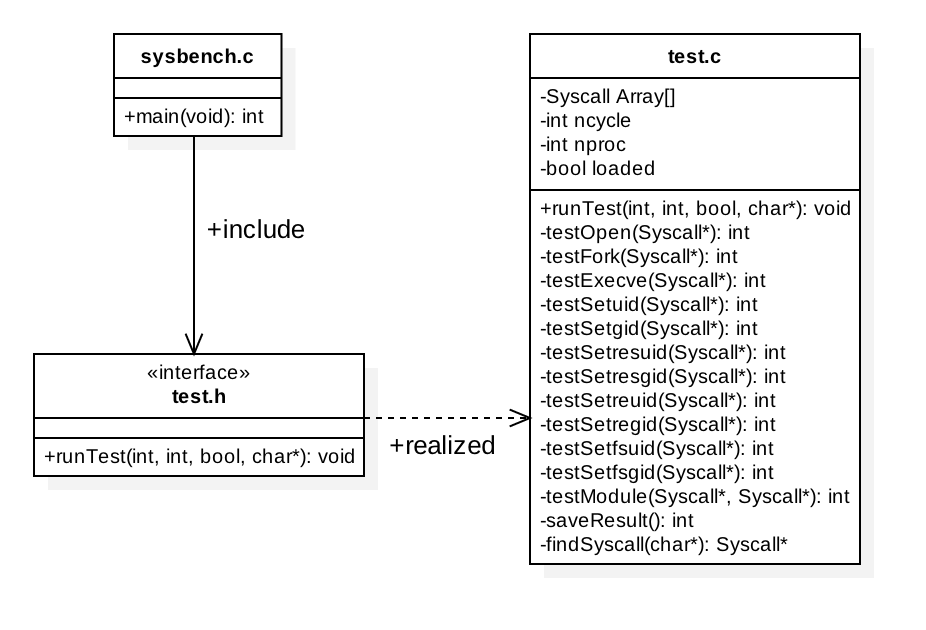
\includegraphics[scale=0.3]{Figures/Architecture}
\caption[Architettura del software SysBench]{Architettura del software SysBench.}
\label{fig:Architecture}
\end{figure}

La \autoref{fig:Architecture} mostra la struttura dei file del progetto e la loro interazione. Il \emph{main} è contenuto nel file \emph{sysbench.c}, in cui avviene il setup del programma che comprende la pulizia del prompt dei comandi, al fine di avere la finestra interamente dedicata a SysBench, e la verifica della presenza o meno di LKRG, la quale viene riportata assieme ai risultati nel file di output. Inoltre vengono letti i parametri passati da riga di comando, ovvero il numero di volte \emph{ncycle} che la singola system call verrà testata ed il nome del file \emph{filename} di output in cui vengono salvati i risultati. È importante prestare attenzione ad i parametri inseriti dall'utente, in quanto un malintenzionato potrebbe inserire codice malevolo per apportare modifiche dannose, dato che vengono richiamate funzionalità potenzialmente pericolose come la \emph{setuid()}. In merito a ciò, si è inserito il controllo di tale parametri al file di verificare la loro integrità.

Il file \emph{test.c} è un grosso ed unico sorgente nel quale vengono definite internamente tutte le funzioni utilizzate nel test; infatti, \emph{runTest()} che è l'unica funzione d'interfaccia è composta da un ciclo all'interno del quale vengono eseguite in serie tutte le valutazioni delle varie system call. Per scelta progettuale, si è deciso di creare la struttura \emph{Syscall} che rappresenta le varie chiamate di sistema da eseguire. È composta da:

\begin{itemize}
\item il nome in formato human-readable della funzione;
\item il puntatore alla funzione da eseguire, per fare si che ognuna di esse esegua il test opportuno (esempio: alla Syscall che testa la \emph{open()} verrà assegnato il test \emph{testOpen()} durante la creazione);
\item il tempo di esecuzione del test misurato in doppia precisione.
\end{itemize}

Durante la fase di progettazione del sistema si è prestata maggiore attenzione alla scalabilità, ovvero la possibilità di aggiungere/rimuovere funzionalità in maniera semplice ed efficace in base alle proprie esigenze. Grazie alla struttura del programma, è possibile aggiungere un ulteriore test di un'altra system call in maniera facile ed immediata: è sufficiente dichiarare una nuova Syscall all'interno dell'array in fase di inizializzazione, implementare la propria funzione \emph{testX()} ed assegnarla correttamente. Il sistema si preoccupa di soddisfare tutte le Syscall presenti, salvando il risultato di ognuna di esse independentemente dal numero.

Per risparmiare tempo, si è deciso di effettuare contemporaneamente sia il test di caricamento modulo sia quello di rimozione, in quanto non avrebbe senso scorporarli per il semplice motivo che il programma se deve effettuare l'inserimento di un modulo X volte, dovrà effettuare la sua rimozione altrettante volte al fine di non ricevere errore dalla funzione \emph{insert\_module()}, la quale fallisce se il target è già caricato nel kernel. Per questo è stata creata una funzione di utility \emph{findSyscall()}, la quale serve per ottenere il puntatore alla Syscall opposta a quella che si sta eseguendo (esempio: si sta testando la \emph{insert\_module()}, si deve trovare il puntatore alla \emph{delete\_module()} e viceversa), in maniera tale da salvare direttamente il risultato della funzione complementare all'interno della sua struttura.

Le funzionalità \emph{fork()} ed \emph{execve()} lavorano in maniera leggermente differente dalle altre; mentre solitamente la system call viene eseguita ncycle-volte come inserito dall'utente, queste due funzioni devono tenere conto del limite di processi istanziati dall'utente. È infatti possibile osservare tale limite leggendo il file \emph{/proc/self/limits} in cui vi è indicato il valore massimo oppure un'apposita struttura in C contenente tutti i limiti del sistema. Una volta letto questo valore, bisogna tenere conto anche dei processi al momento attivi nel sistema e la possibilità di lanciarne altri durante l'esecuzione di SysBench; per questo se il numero inserito dall'utente è troppo grande, fork() ed execve() potranno creare al massimo $ LIM / 2$, dove LIM è il valore letto in precedenza.

La system call \emph{execve()}, come riportato nella parte finale del capitolo precedente, sovrascrive tutto lo spazio dedicato al processo chiamante per eseguirne un altro e ciò potrebbe essere un problema dato che significherebbe la terminazione di SysBench non appena viene richiamata tale funzione. Come soluzione, si è scelto di far eseguire il comando ad un processo figlio, generato mediante la fork(), ottenendo così come tempo finale d'esecuzione la somma delle due chiamate a funzione. Quest'ultima feature è possibile grazie alla sincronizzazione tra i processo 'padre' ed i 'figli' utilizzando la funzione \emph{wait()}, grazie la quale il chiamante attende che tutti i suoi figli notifichino la loro terminazione, e solo in seguito procede con l'esecuzione del suo codice. Con questa soluzione non solo si riesce a misurare abbastanza accuratamente il tempo d'esecuzione dell'intera chiamata a funzione, ma il programma non genera dei processi definiti 'zombie', ossia processi creati e non terminati che rimangono in memoria in attesa di essere rimossi consumando inutilmente risorse

\section{Caso d'uso}

Essendo SysBench un software d'utility sviluppato per un utilizzo semplice e mirato, l'unico caso d'uso da commentare è il seguente mostrato in \autoref{fig:UseCase}.

\begin{figure}[!htbp]
\centering
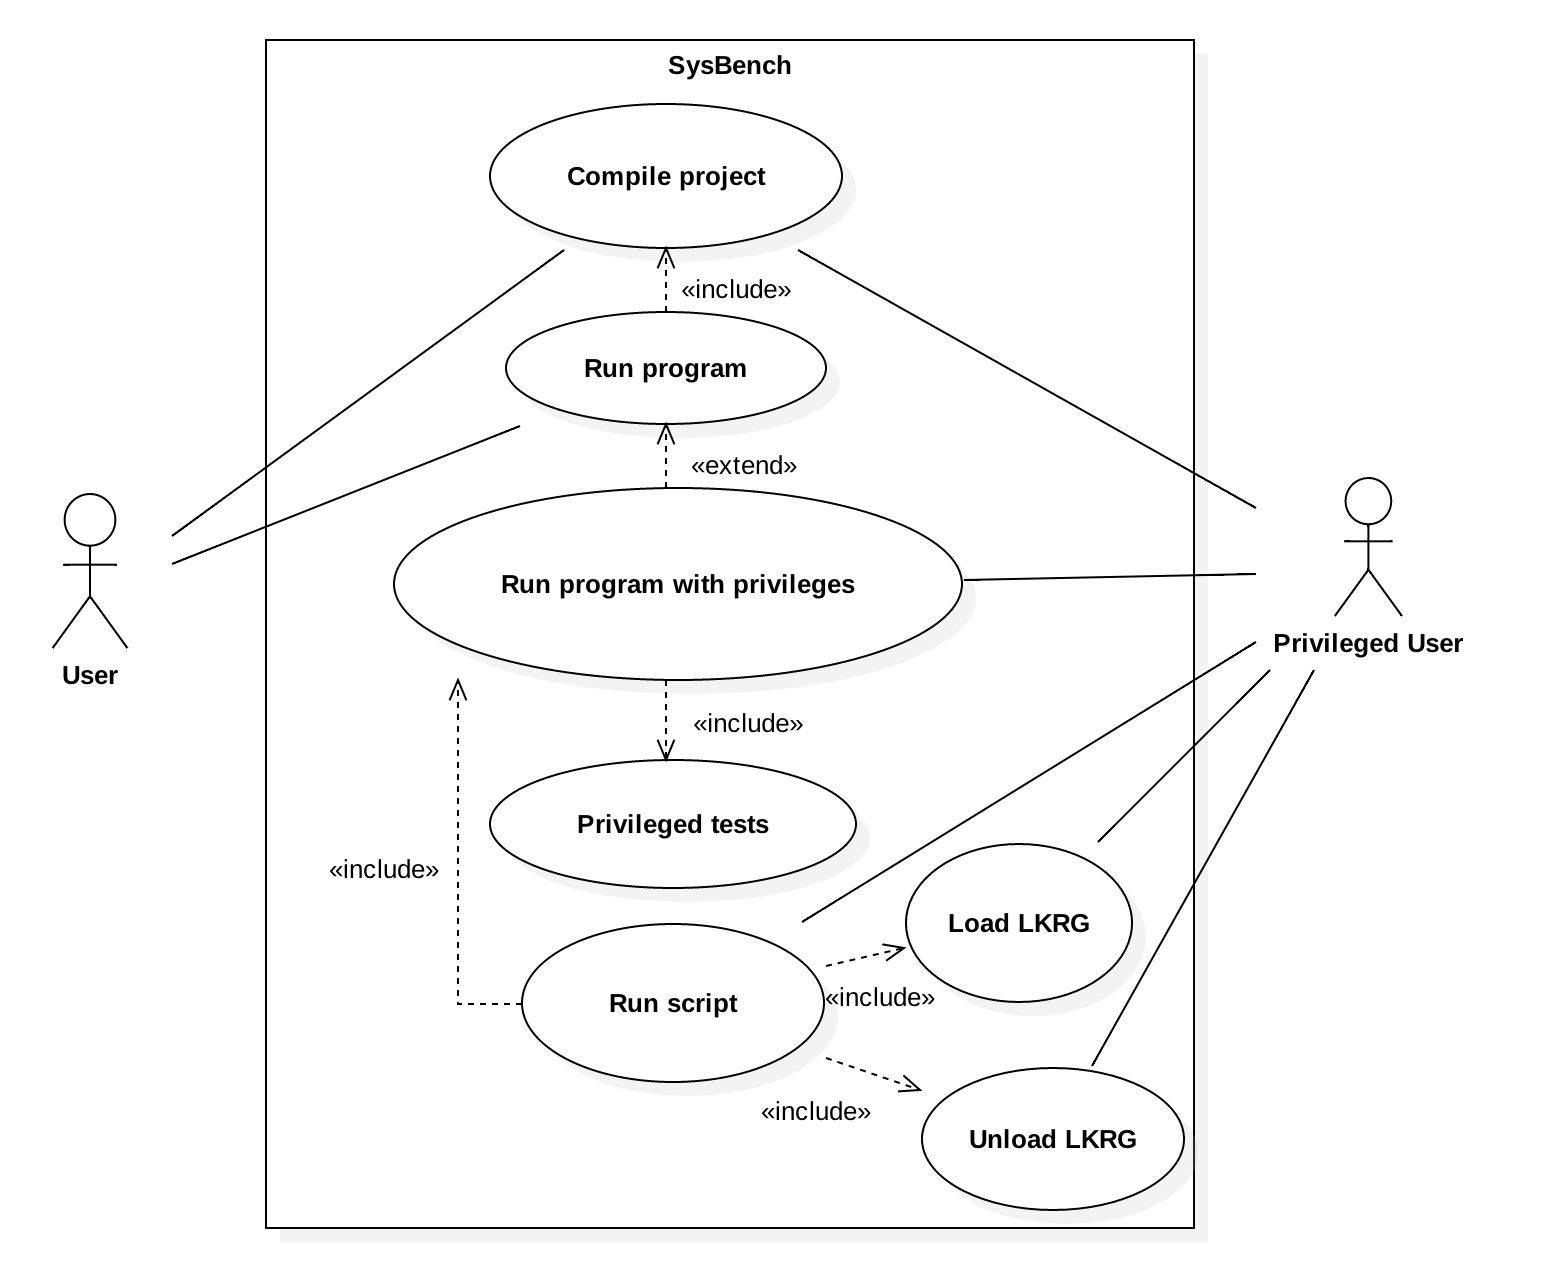
\includegraphics[scale=0.28]{Figures/UseCase}
\caption[Diagramma UML dei casi d'uso di SysBench]{Diagramma UML dei casi d'uso di SysBench.}
\label{fig:UseCase}
\end{figure}

Una volta compilato il progetto, è possibile procedere con due diverse modalità di esecuzione:

\begin{enumerate}
\item normal mode (\emph{./sysbench ncycle filename});
\item sudo mode (\emph{sudo ./sysbench ncycle filename})
\end{enumerate}
dove ncycle corrisponde al numero di volte che una singola chiamata di sistema viene invocata, mentre filename è il nome del file in cui verrano salvati i risultati all'interno della cartella \emph{output}, creata automaticamente nel caso non fosse già presente.

La differenza risiede nei test delle funzionalità di caricamento e rimozione modulo, ovvero \emph{testMoule()} (il quale richiama le system call \emph{insert\_module()} e \emph{delete\_module}); non è infatti possibile eseguire con successo questo test se non si hanno i privilegi di root, in quanto per scelta di sicurezza del sistema queste system call non possono modificare i moduli caricati nel kernel se eseguite da un normale utente (non a caso anche i comandi \emph{insmod} e \emph{rmmod} mostrati nel Capitolo I necessitano di tali privilegi).

Ad esclusione di questo test, tutti gli altri sono effettuati con successo in entrambe le modalità e falliscono solamente nel caso vi sia un errore interno al sistema. Nonostante l'utilizzo di sudo permetta di effettuare operazioni ritenute malevole da LKRG quindi non buone per il sistema, in questo progetto tutte le system call testate che prevedono un'alterazione di un parametro del processo si limitano ad impostare come valore dell'attributo quello corrente, in maniera tale da terminare con successo: ad esempio la \emph{setuid()}, utilizzata per cambiare l'identificatore dell'utente che ha lanciato il processo, imposta tale parametro al valore ritrovato in seguito alla system call opposta, ovvero \emph{getuid()}.

Vi è inoltre un'altra modalità d'esecuzione che prevede il caricamento e rimozione automatica di LKRG tra una valutazione di SysBench ed un'altra. Nel progetto è presente infatti uno script che richiede i privilegi di root per essere eseguito (per il motivo appena spiegato), grazie al quale viene eseguito il benchmark un numero di volte a piacere dall'utente. Si è infatti osservato che la differenza tra un'esecuzione singola di SysBench con ncycle=50 e 50 esecuzioni con ncycle=1 presentano risultati completamente differenti introdotti nel prossimo capitolo. Questa differenza è dovuta dalle ottimizzazioni e salvataggio in memoria cache delle funzioni invocate che permettono la loro immediata esecuzione, risparmiando al programma la loro ricerca nella tabella delle system call. È possibile eseguire lo script da riga di comando lanciando \\\emph{sudo ./script.sh ntimes ncycle path/to/p\_lkrg.ko} dove:

\begin{itemize}
\item ntimes è il numero di volte che verrà effettuato il benchmark;
\item ncycle è il numero di chiamate alle singole system call in ogni benchmark;
\item path/to/p\_lkrg.ko è il percorso del modulo compilato nel proprio sistema.
\end{itemize}

Nonostante i risultati ottenuti siano differenti, la possibilità di eseguire il programma con il parametro ncycle maggiore di 1 è stata volutamente lasciata, perchè i valori non solo sono interessanti per futuri sviluppi del progetto, ma anche per un'analisi delle ottimizzazioni di un calcolatore esterna a questo elaborato.
\chapter{Analisi delle performance}

\label{Chapter4}

In questo capitolo interamente tecnico vengono presentati i risultati ottenuti in seguito alla valutazione di tre sistemi Linux differenti. Essendo tra le versioni più conosciute ed utilizzate al momento, si è deciso di effettuare il benchmark in Ubuntu, Debian e Mint in ambiente virtuale utilizzando come software per la creazione delle macchine VirtualBox. Si definisce il computer fisico \emph{host}, in quanto mette a disposizione il proprio spazio e l'hardware per virtualizzare il sistema definito \emph{guest} creato con VirtualBox.

Al fine di ottenere risultati confrontabili è necessario che durante la fase di testing non solo l'host rimanga nella medesimo stato per ogni guest, ovvero stessi programmi/processi in esecuzione, memoria, cpu disponibile ed altri valori, ma anche i guest devono eseguire il benchmark con le stesse risorse allocate.

Nella tabella sottostante vi sono le specifiche dei sistemi utilizzati:

\begin{table}[!htbp]
\label{tab:specs}
\centering
\begin{adjustbox}{width=\textwidth}
\begin{tabular}{|c|c|c|c|c|c|c|}
\hline
\textbf{Tipo} & \textbf{Modello} & \textbf{Sistema Operativo} & \textbf{Kernel} & \textbf{RAM(GB)} & \textbf{CPU} & \textbf{Core} \\
\hline
Host & MacbookPro (2015) & High Sierra v10.13.6 & Darwin v17.7.0 & 16 & IntelCore i7-4770HQ 2.2GHz & 4 \\
\hline
Guest & "" & Ubuntu v16.04.5 & Linux v4.15.0-29-generic &  2 & "" & 1 \\
\hline
Guest & "" & Debian v4.04.5 & Linux v4.9.0-7-amd64 &  2 & "" & 1 \\
\hline
Guest & "" & Mint v19 & Linux v4.15.0-20-generic &  2 & "" & 1 \\
\hline
\end{tabular}
\end{adjustbox}
\caption{Specifiche dei sistemi utilizzati}
\end{table}

Nonostante nella pagina di LKRG l'autore proponga gli esempi di rilevazione software solamente in ambiente Ubuntu v16.04, si è deciso di effettuare un'analisi anche nelle altre due distribuzioni, per poter osservare in che modo reagissero al caricamento del modulo e soprattutto se nella stessa maniera, oppure con qualche differenza. Dovendo testare system call comuni a tutte le distribuzioni Linux, non vi è alcun problema di compatibilità nell'utilizzo di SysBench nei tre guest.

In alcune verifiche effettuate è risultata una netta differenza di tempi d'esecuzione delle funzioni con LKRG attivo e non, per cui volendo confrontare dei dati così diversi si è scelto di utilizzare una scala logaritmica per l'asse delle ordinate (y) o delle ascisse (x) a seconda della tipologia di grafico. È importante sottolineare questo dettaglio, perchè la lettura del grafico è leggermente differente: mentre solitamente osservando l'asse y notiamo un aumento caratterizzato da step lineari (esempio: 1, 2, 3, ..., 10), utilizzando la scala logaritmica la distribuzione dei valori è differente, in quanto la distanza tra i punti è calcolata utilizzando il logaritmo secondo la legge $\lambda (OA)= \log (a)$ che rappresenta a distanza tra un punto di coordinata (0, a) e l'origine dell'asse y O è data da .

Prendiamo come esempio la scala logaritmica in base 10 utilizzata in questo elaborato osservando la figura sottostante in cui vi sono riportate alcune potenze:

\begin{figure}[!ht]
\centering
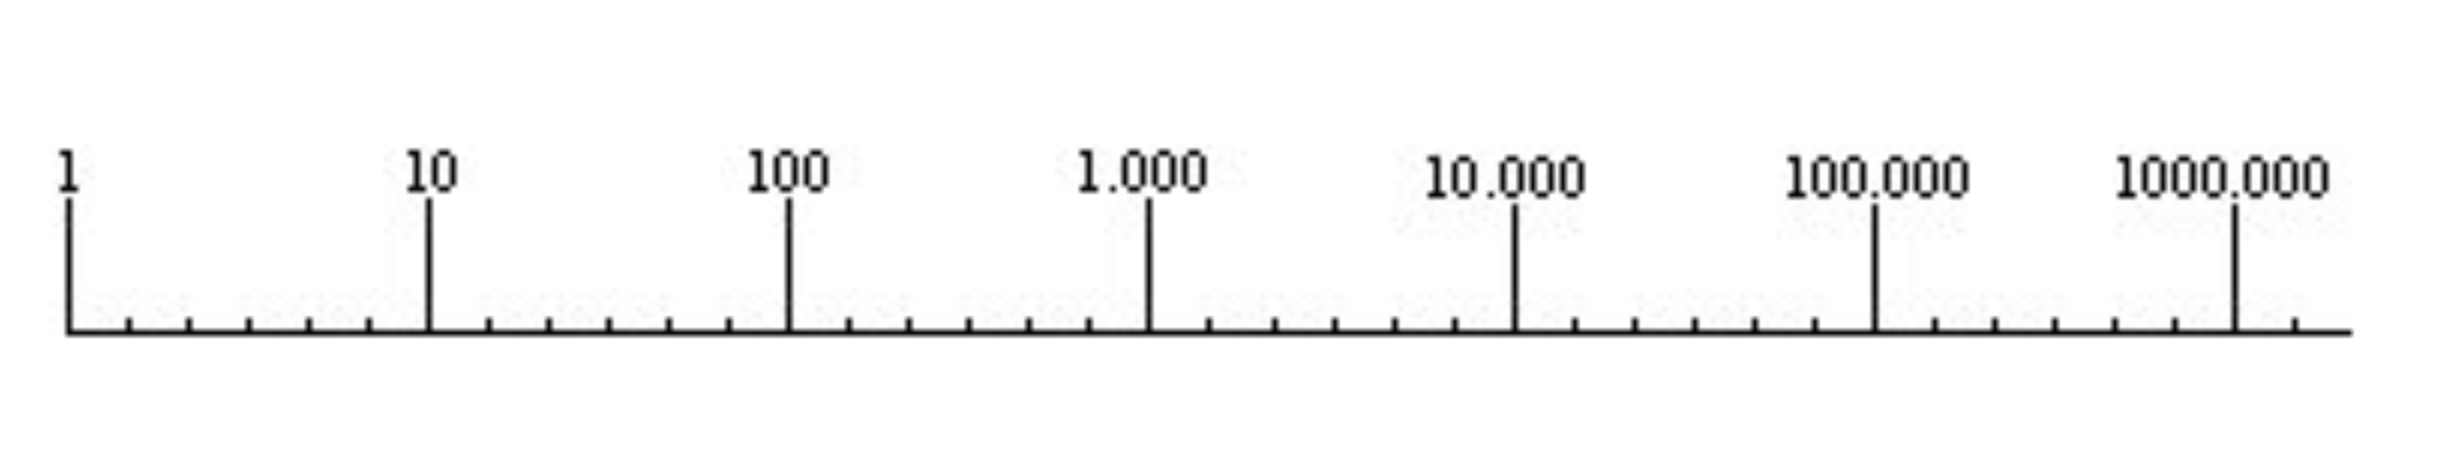
\includegraphics[scale=0.2]{Figures/LogarithmicScale}
\caption[Scala logaritmica di base 10.]{Scala logaritmica di base 10.\\Fonte: \href{https://it.wikipedia.org/wiki/Scala_logaritmica}{https://en.wikipedia.org}}
\label{fig:logarithmicScale}
\end{figure}

Il valore \emph{1} è calcolabile come la distanza tra il punto d'origine O e sé stesso, ovvero: $\lambda (OO) = 0 => \log (x_0) = 0 => x_0 = 1$. Ugualmente il valore \emph{10} che rappresenta il primo step è dato da $\lambda (OA) = 1 => \log (x_1) = 1 => x_1 = 10$.

Essendo abituati alla scala lineare, verrebbe da pensare che il punto medio tra l'1 ed il 10 di distanza 0.5 dall'origine rappresenti il valore 5; in realtà nella scala logaritmica applicando il calcolo si ottiene $\lambda (OM) = 0.5 => \log (x_m) = 0.5 => x_m = 1/\sqrt{10} \approx 3.16$.

In questa maniera è vero che si perde un po' di precisione del dato, ma è possibile raffigurare valori estremamente differenti, persino con ordini di grandezza doppi o tripli.

Al fine di una buona lettura, si ricorda che in ogni grafico sono riportati i parametri \emph{ncycle} ed \emph{nproc}, i quali corrispondono al numero di singole system call invocate e processi creati (esempio: ncycle=100 significa che la system call X è stata eseguita 100 volte). Inoltre nei grafici sono stati utilizzati i simboli matematici per indicare:

\begin{itemize}
\item \bm{$\sigma$}: la deviazione standard, ovvero l'indice di dispersione dei dati rispetto la media aritmetica;
\item \bm{$\overline{x}}$: per indicare il tempo di esecuzione medio della singola system call, calcolato dividendo i tempi ottenuti per il numero di system call invocate.
\end{itemize}

Infine, i risultati presentati sono stati ricavati mediante diversi test, in alcuni dei quali certe system call hanno un tempo d'esecuzione pari a 0. Per coerenza si è deciso di non rimuovere tali informazioni nei grafici, nonostante possa sembrare leggermente più complessa la lettura dei valore lungo l'asse delle y. Pertanto quando lungo tale asse è indicato il valore $0.00e^{+0}$, si prenda come riferimento per i valori leggermente superiori l'ordine di grandezza $1.00e^{-7}$, il secondo valore più piccolo misurato.

%----------------------------------------------------------------------------------------
%	UBUNTU TESTS
%----------------------------------------------------------------------------------------
\section{Test in Ubuntu}

L'analisi di LKRG in Ubuntu ha presentato risultati interessanti, soprattutto confrontando le diverse modalità d'esecuzione del programma. Iniziamo osservando il grafico sottostante, ottenuto eseguendo lo script mediante il quale avvengono 50 esecuzioni consecutive di SysBench con ncycle=1 (e non una singola esecuzione con ncycle=50 che verrà discussa in seguito), salvando i risultati in altrettanti file di output. In questo modo non vi possono essere ottimizzazioni dovuti alla cache, in quanto essendo una memoria veloce e piccola in cui vengono memorizzati i dati recentemente usati dalla memoria principale (RAM), ogni volta che la system call viene invocata il sistema salva le informazioni relative a tale funzione nella cache, ma non ne farà uso per il semplice motivo che il programma richiama la funzione una singola volta, mentre come vedremo in seguito tale memoria incide sul tempo d'esecuzione nel caso la stessa esecuzione richiami la system call più volte.

\begin{figure}[!ht]
\centering
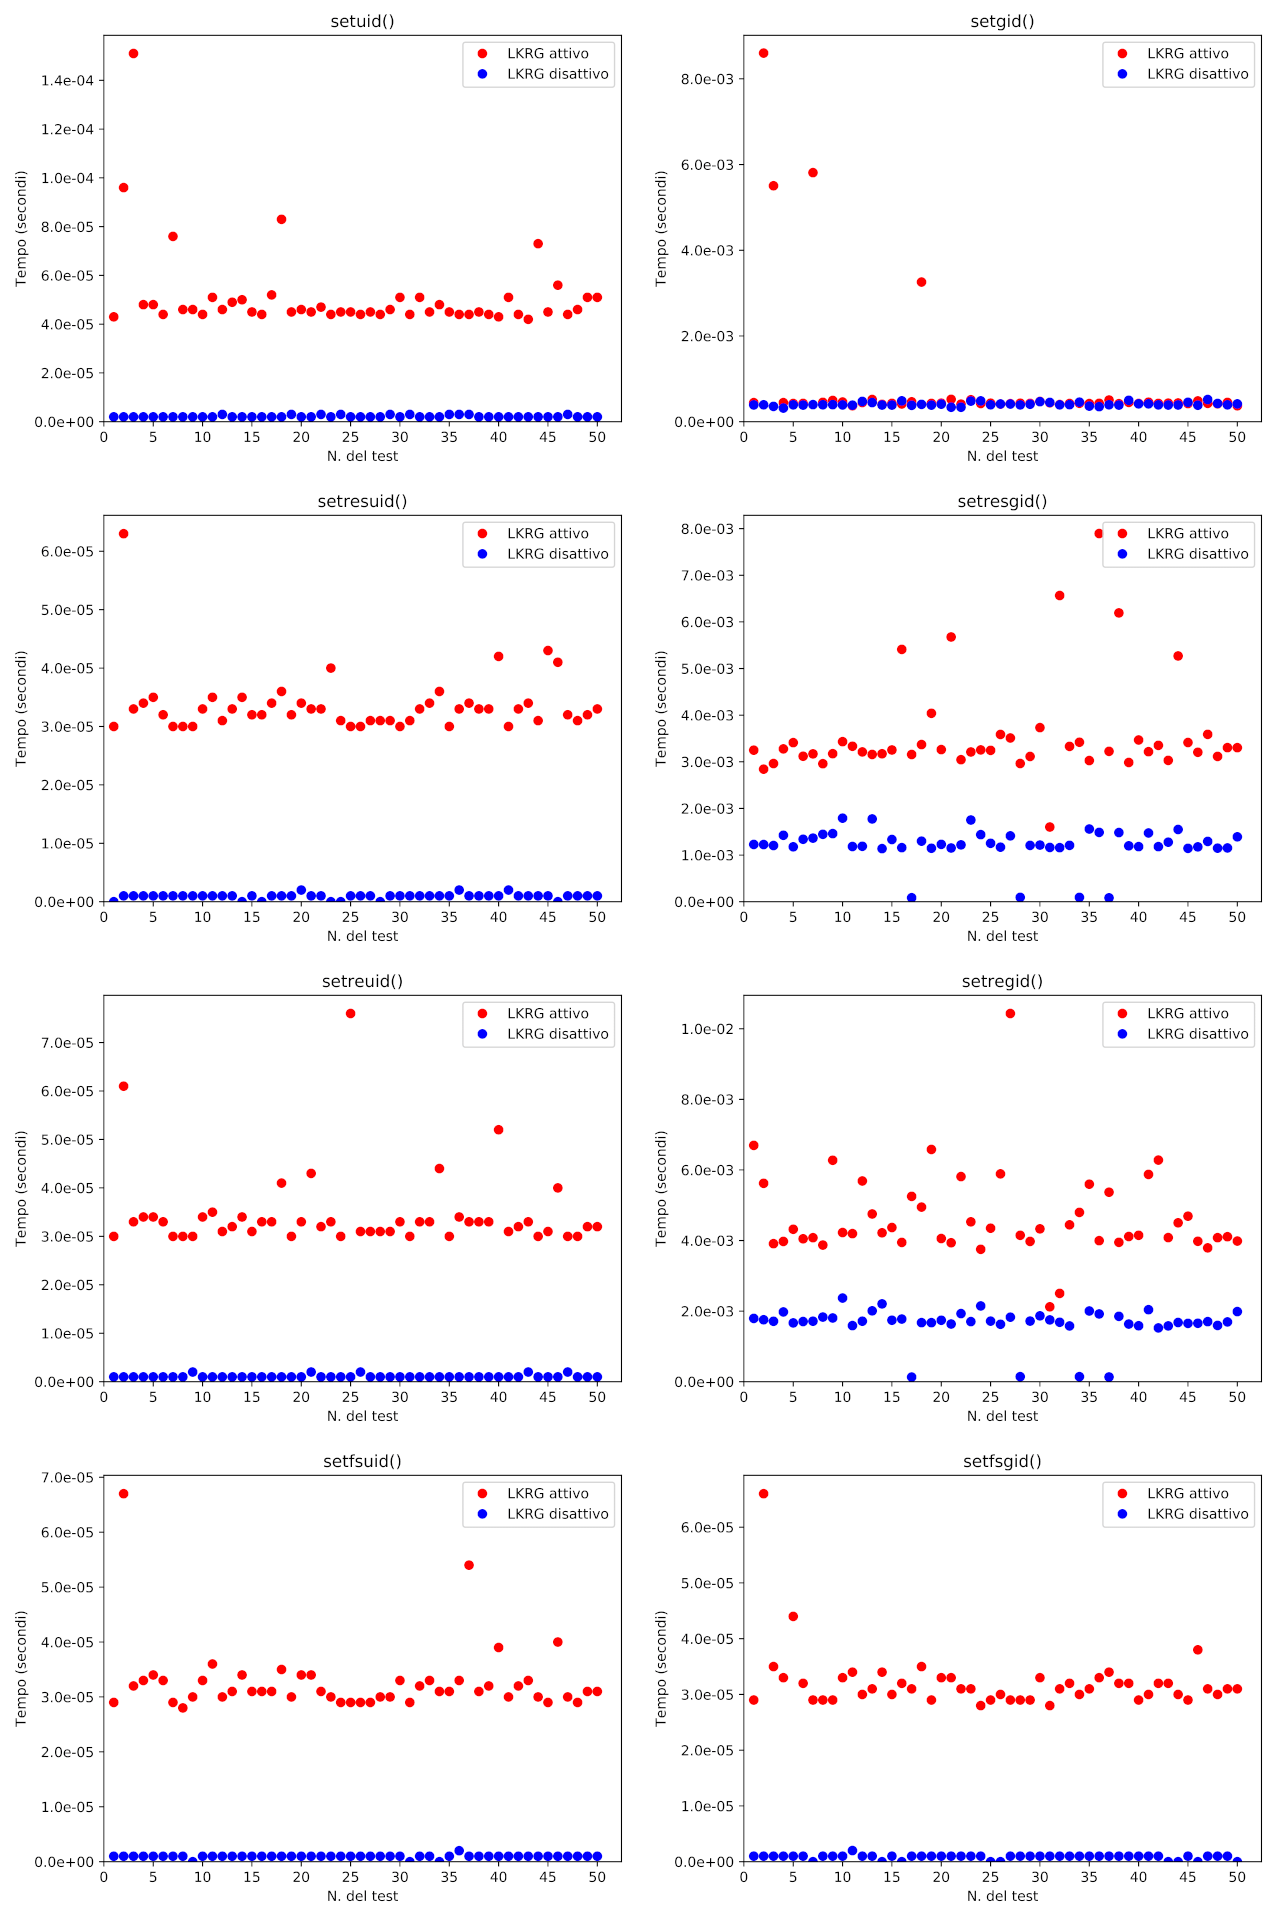
\includegraphics[scale=1.15]{Figures/Ubuntu/SingleSet}
\caption[Benchmark funzioni \emph{setX} con ncycle=1 (Ubuntu)]{Benchmark funzioni \emph{setX} con ncycle=1 (Ubuntu).}
\label{fig:setxUbuntuFig}
\end{figure}

Nella \autoref{fig:setxUbuntuFig} sono mostrati i risultati dei test delle funzionalità indicate con \emph{setX()} che alterano i parametri del processo, dove X è il parametro stesso (esempio: uid). Si noti come l'unica system call il cui tempo d'esecuzione non è rilevantemente influenzato dalla presenza di LKRG sia la \emph{setgid()}, i cui risultati mostrano come rimanga circa costante ad eccezione di qualche test.

Per tutte le altre funzioni, si osserva che la differenza del tempo d'esecuzione con il modulo caricato e modulo non caricato è elevata, passando da un'ordine di grandezza pari a $10^{-6} \approx 0$ nel grafico a $10^{-5}$ tranne nella \emph{setregid()} e \emph{setresgid()} in cui il tempo aumenta ma di fattore $\approx 2$. Tali tempi per il calcolatore sono pressappoco irrilevanti, nonostante graficamente possano avere un impatto diverso e si potrebbe pensare che sia totalmente sconsigliato l'utilizzo di LKRG. Di seguito è riportata la tabella in cui vengono indicate la media e la deviazione standard per ognuna delle system call nel grafico. 

\begin{table}[!htbp]
\centering
\begin{tabular}{|c|c|c|c|c|}
\hline
\textbf{SystemCall} & \bm{$\overline{x}$} \textbf{loaded} & \bm{$\overline{x}$} \textbf{unloaded} & \bm{$\sigma$} \textbf{loaded} & \bm{$\sigma$} \textbf{unloaded}\\
\hline
setuid() & 5.130e-05 & 2.200e-06 & 1.763e-05 & 4.000e-07 \\
\hline
setgid() & 8.679e-04 & 4.079e-04 & 1.549e-03 & 4.176e-05 \\
\hline
setresuid() & 3.366e-05 & 9.200e-07 & 5.152e-06 & 4.400e-07 \\
\hline
setresgid() & 3.577e-03 & 1.210e-03 & 1.052e-03 & 3.700e-04 \\
\hline
setreuid() & 3.458e-05 & 1.100e-06 & 8.183e-06 & 3.000e-07 \\
\hline
setregid() & 4.652e-03 & 1.646e-03 & 1.234e-03 & 4.758e-04 \\
\hline
setfsuid() & 3.270e-05 & 9.600e-07 & 6.306e-06 & 2.800e-07 \\
\hline
setfsgid() & 3.212e-05 & 8.400e-07 & 5.548e-06 & 4.176e-07 \\
\hline
\end{tabular}
\caption{Dati benchmark funzioni \emph{setX} con ncycle=1 (Ubuntu)}
\label{table:setxUbuntuData}
\end{table}

Si osservi l'enorme differenza che vi è non solo tra il tempo medio della singola chiamata, ma anche tra la deviazione standard, ovvero l'indice di dispersione statistico che indica quanto mediamente i dati si discostano dalla media stessa. La differenza tra la deviazione standard con LKRG caricato e non è sempre almeno di un ordine di grandezza, ad eccezione della prima funzione in cui è persino due ordini. L'incremento dei tempi d'esecuzione delle system call suggeriscono l'effettivo intervento del modulo, il quale compiendo i propri controlli d'integrità aggiunge sicuramente ulteriore tempo alla chiamata a funzione.

I grafici in \autoref{fig:othersUbuntuFig} e i dati nella \autoref{table:othersUbuntuData} riportano i risultati delle restanti system call testate nelle stesse medesime condizioni. Mentre i grafici delle funzionalità \emph{open()}, \emph{fork()} e \emph{delete\_module()} presentano una distribuzione dei dati simili a quelle analizzate in precedenza, quella della \emph{insert\_module()} è molto differente, in quanto i tempi variano ragionevolmente in entrambe le situazioni di testing. Mediamente il tempo d'esecuzione con LKRG è superiore, ma come si può notare talvolta può impiegare più tempo quando il modulo non è presente, in quanto incidono numerosi fattori nell'esecuzione di questa chiamata legati al caricamento dinamico di un modulo nel kernel; infatti è interessante osservare che la deviazione standard misurata è maggiore quando il modulo non è caricato. È dunque possibile, come nel nostro caso, che nonostante LKRG sia attivo il sistema impieghi meno tempo a caricare un modulo rispetto a quando non lo sia.

\begin{table}[!htbp]
\centering
\begin{tabular}{|c|c|c|c|c|}
\hline
\textbf{SystemCall} & \bm{$\overline{x}$} \textbf{loaded} & \bm{$\overline{x}$} \textbf{unloaded} & \bm{$\sigma$} \textbf{loaded} & \bm{$\sigma$} \textbf{unloaded}\\
\hline
open() & 3.398e-05 & 1.100e-06 & 5.006e-06 & 3.000e-07 \\
\hline
fork() & 3.518e-05 & 1.260e-06 & 4.117e-06 & 4.386e-07 \\
\hline
execve() & 7.740e-06 & 6.300e-06 & 2.234e-06 & 1.389e-06 \\
\hline
insert\_module() & 9.532e-02 & 6.940e-02 & 1.180e-02 & 1.587e-02 \\
\hline
delete\_module() & 3.226e-05 & 9.400e-07 & 4.837e-06 & 4.200e-07 \\
\hline
\end{tabular}
\caption{Dati benchmark restanti funzioni con ncycle=1 (Ubuntu)}
\label{table:othersUbuntuData}
\end{table}

\begin{figure}[!ht]
\centering
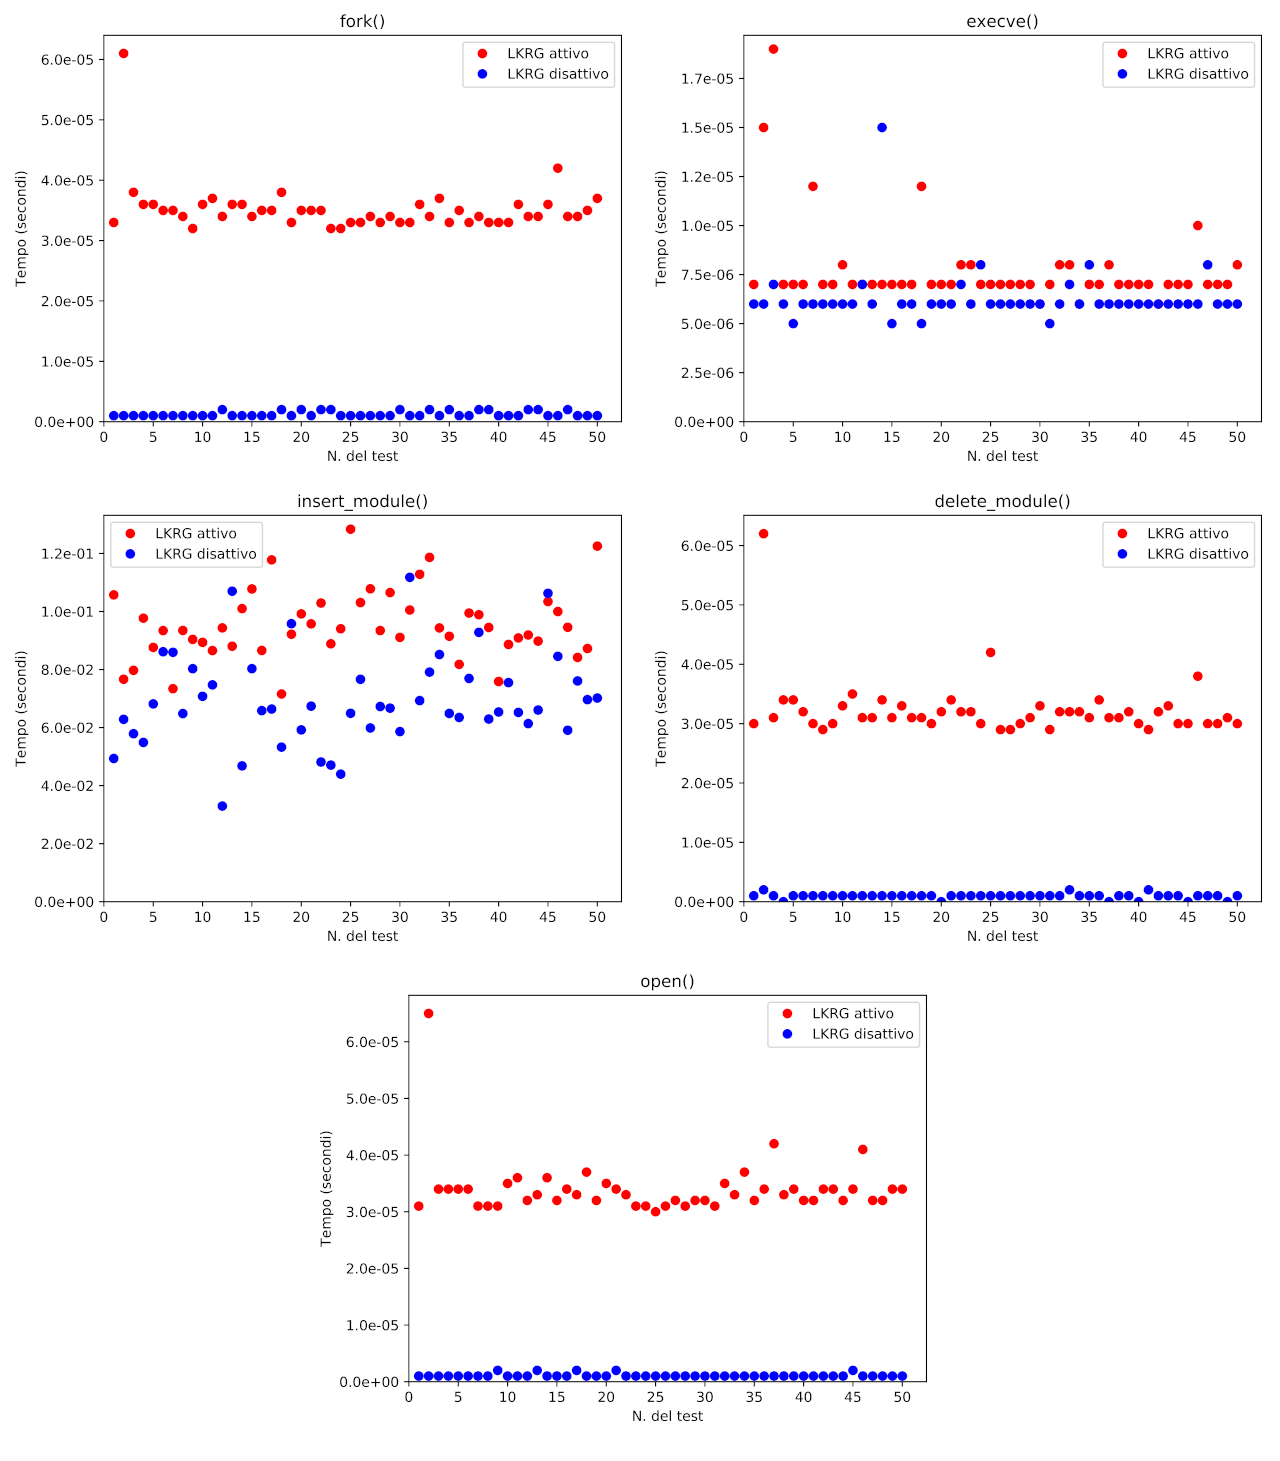
\includegraphics[scale=1.3]{Figures/Ubuntu/SingleOthers}
\caption[Benchmark restanti system call con ncycle=1 (Ubuntu)]{Benchmark restanti system call con ncycle=1 (Ubuntu).}
\label{fig:othersUbuntuFig}
\end{figure}

Anche la \emph{execve()} ha un range di valori differenti dalle altre system call, nonostante la distribuzione sia molto simile. Sicuramente LKRG aggiunge del tempo effettuando i suoi controlli, ma la parte più consistente di questa funzione è il reset di memoria del processo corrente, effettuando la sovrascrittura delle vecchie risorse con delle nuove dedicate al comando indicato come parametro. È dunque possibile, come nel nostro caso, che nonstante LKRG sia attivo il sistema impieghi meno tempo ad allocare le risorse al nuovo processo, per vari motivi di scheduling, disponibilità delle risorse o ottimizzazioni. Mediamente si può affermare che il tempo misurato con LKRG è superiore di circa il 22\% il tempo misurato senza.

In generale i dati nella \autoref{table:othersUbuntuData} sono consistenti con quelli nella \autoref{table:setxUbuntuData}: il tempo di certe funzionalità come la rimozione del modulo cambia di fattore $\approx 10$, mentre in altre la differenza è minore.
\\\par

Analizziamo ora come cambiano i tempi d'esecuzione lanciando singolarmente il programma SysBench con ncycle=1, 10, 100, 1000 e 10000 per capire perchè i risultati medi ottenuti possano essere così diversi rispetto a più esecuzioni con lo stesso parametro. Più semplicemente, la differenza tra le due esecuzioni si può riassumere nei seguenti comandi:

\begin{itemize}
\item \emph{sudo ./script.sh 10000 1 path/to/p\_lkrg.jo}, dove 10000 sono le volte che verrà richiamato il programma Sysbench e 1 corrisponde al parametro ncycle;
\item \emph{sudo ./sysbench 10000 filename}.
\end{itemize} 

Senza consultare alcun risultato, possiamo aspettarci di ottenere due output differenti, influenzati dalle ottimizzazioni del processore. L'obiettivo dunque è verificare che il valore della singola system call misurato richiamandola 10000 volte all'interno dello stesso programma sia effettivamente inferiore della media dei valori ottenuti mediante 10000 esecuzioni in cui viene eseguita una volta sola.

\begin{figure}[!ht]
\centering
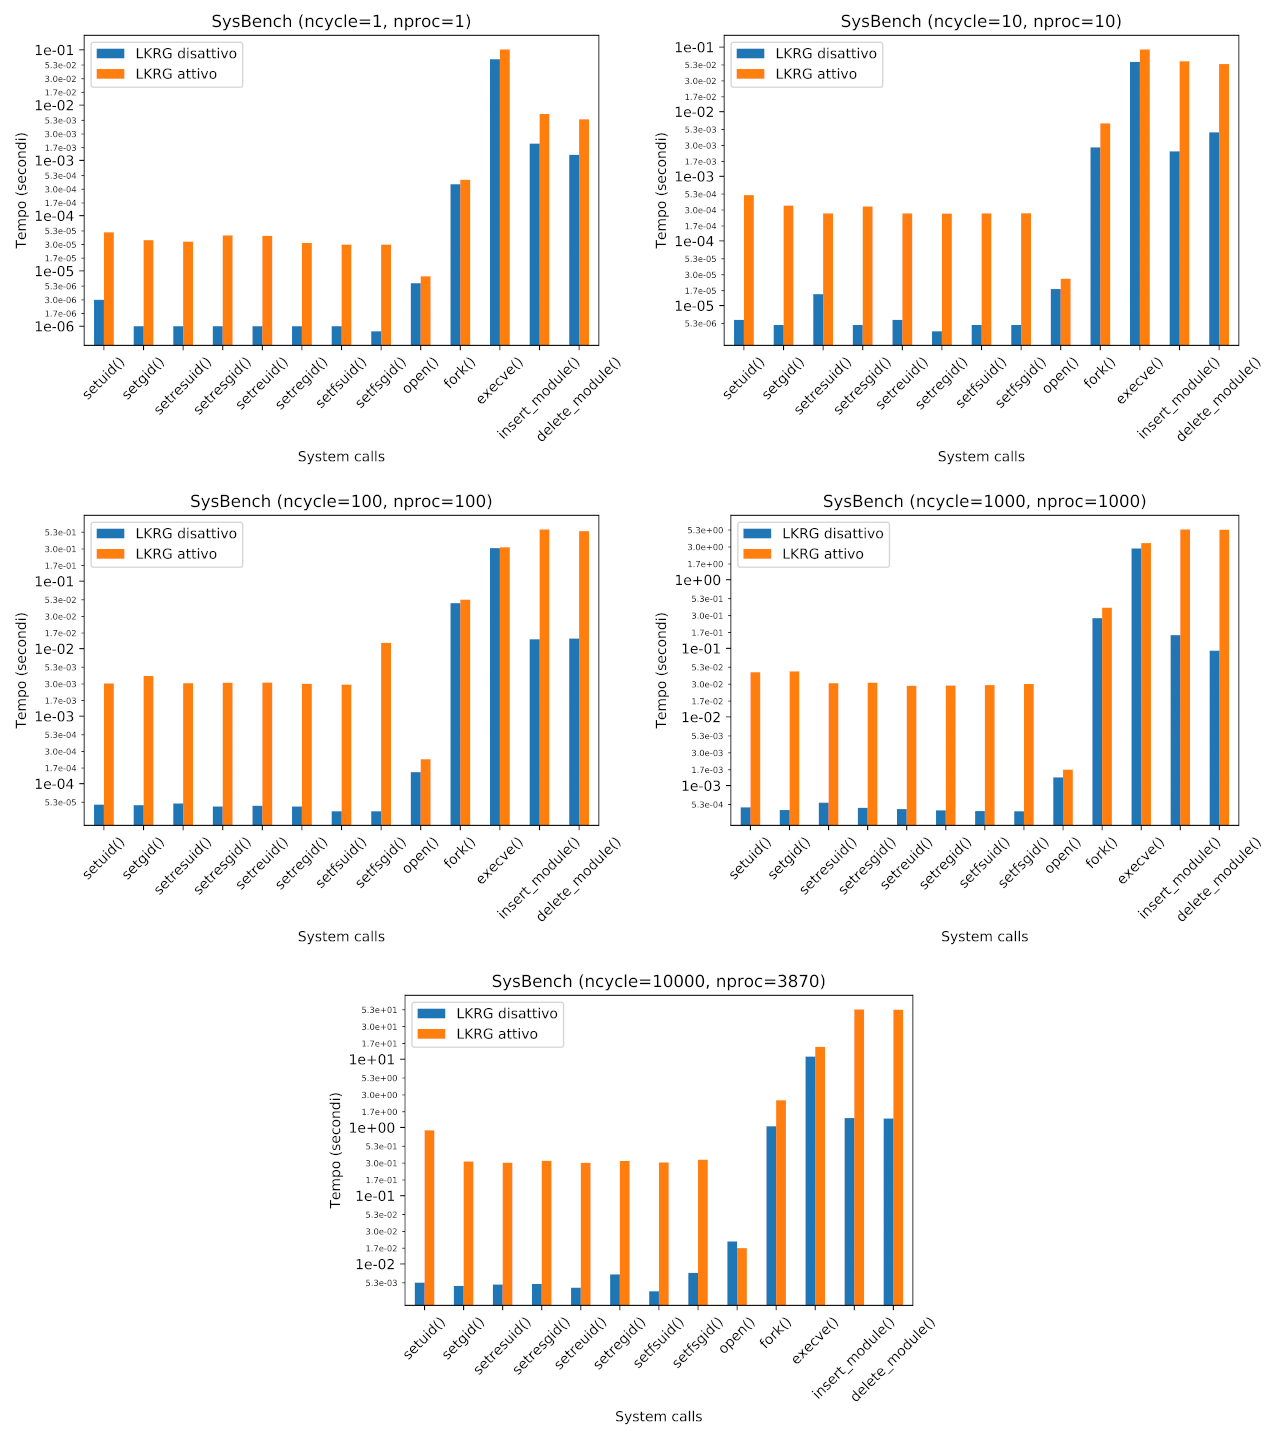
\includegraphics[scale=1.4]{Figures/Ubuntu/Total}
\caption[Benchmark tempo totale (Ubuntu)]{Benchmark tempo totale (Ubuntu).}
\label{fig:totUbuntuFig}
\end{figure}

Iniziamo commentando la \autoref{fig:totUbuntuFig}, raffigurante il tempo totale d'esecuzione delle system call nelle 5 esecuzioni con ncycle differente. Per l'asse delle ordinate (y) si è utilizzato una scala logaritmica, al fine di riuscire ad inserire tutti i dati nello stesso grafico, sebbene siano molto discostanti tra loro.

Si può osservare il tempo aggiunto dalla presenza di LKRG semplicemente sottraendo alle barre arancioni le corrispettive blu. In quasi tutte le funzioni ad eccezione della \emph{fork()}, \emph{execve()} e \emph{open()} l'overhead aggiunto dal modulo è significativo ed aumenta sempre di più al variare del numero di chiamate. È da premettere che tali test sono specifici per questa analisi, al fine di comprendere il lavoro del modulo LKRG, ma in una situazione reale è altamente improbabile trovare un programma che effettui così tante volte consecutive la medesima chiamata.

L'unica che potrebbe raffigurare uno scenario reale è la \emph{open()}, in quanto moltissimi programmi lavorano con più file, aprendoli e chiudendoli diverse volte, ma i grafici e le tabelle presenti in questa trattazione suggeriscono che tale system call sia leggermente influenzata da LKRG a differenza di molte altre, tra cui la \emph{insert\_module()}. Infatti quest'ultima funzione e la sua opposta \emph{delete\_module()} risentono dei controlli d'integrità, aumentando il loro tempo d'esecuzione di circa mezzo ordine di grandezza; se nei primi grafici i loro tempi con LKRG attivo sono inferiori a quelli della \emph{execve()}, negli ultimi in cui ncycle è molto più grande superano qualsiasi tempo d'esecuzione delle altre system call, in quanto si somma ncycle-volte l'overhead aggiunto dal modulo, il quale risulta essere massimo per queste due funzioni. Infine, un'altra differenza facile da notare sono i tempi delle funzioni \emph{setX}; nonostante essi siano molto più piccoli delle altre funzionalità, si può affermare che in percentuale sono quelle maggiormente influenzate, in quanto il rapporto tra i tempi è pari a $1.5x10^{1}$ per la \emph{setuid()} e persino maggiore per le altre.

\begin{table}[!htbp]
\centering
\begin{tabular}{|c|c|c|c|c|}
\hline
\textbf{SystemCall} & \bm{$\overline{x}$} \textbf{loaded} & \bm{$\overline{x}$} \textbf{unloaded} & \bm{$\sigma$} \textbf{loaded} & \bm{$\sigma$} \textbf{unloaded}\\
\hline
setuid() & 5.349e-05 & 1.021e-06 & 2.007e-05 & 9.903e-07 \\
\hline
setgid() & 3.772e-05 & 5.793e-07 & 4.858e-06 & 2.112e-07 \\
\hline
setresuid() & 3.059e-05 & 8.148e-07 & 2.326e-06 & 3.895e-07 \\
\hline
setresgid() & 3.467e-05 & 5.885e-07 & 4.780e-06 & 2.065e-07 \\
\hline
setreuid() & 3.197e-05 & 5.945e-07 & 5.749e-06 & 2.102e-07 \\
\hline
setregid() & 2.994e-05 & 6.001e-07 & 2.144e-06 & 2.269e-07 \\
\hline
setfsuid() & 2.919e-05 & 5.426e-07 & 1.369e-06 & 2.319e-07 \\
\hline
setfsgid() & 4.847e-05 & 5.724e-07 & 3.667e-05 & 1.707e-07 \\
\hline
open() & 3.263e-06 & 2.547e-06 & 2.394e-06 & 1.749e-06 \\
\hline
fork() & 5.349e-04 & 3.333e-04 & 1.067e-04 & 7.851e-05 \\
\hline
execve() & 2.428e-02 & 1.645e-02 & 3.877e-02 & 2.558e-02 \\
\hline
insert\_module() & 5.907e-03 & 5.380e-04 & 5.558e-04 & 7.400e-04 \\
\hline
delete\_module() & 5.430e-03 & 4.213e-04 & 8.738e-05 & 4.404e-04 \\
\hline
\end{tabular}
\caption{Dati benchmark con ncycle=1, 10, 100, 1000, 10000 (Ubuntu)}
\label{table:totUbuntuData}
\end{table}

Confrontando i dati della \autoref{table:totUbuntuData} con quelli delle tabelle ottenute precedentemente (\autoref{table:othersUbuntuData} e \autoref{table:setxUbuntuData}) si osserva l'enorme differenza del tempo medio d'esecuzione (\bm{$\overline{x}}$) delle funzioni in entrambi i casi, potendo pensare che vi sia un errore nella misurazione. In realtà la differenza è dovuta all'insieme delle ottimizzazioni apportate dal processore e dalla memoria cache non trattate in questo elaborato. Una buona idea per uno possibile sviluppo è quella di estendere la trattazione analizzando il comportamento del modulo in processori differenti, capendo le modifiche apportate da ognuno analizzando ogni singolo step d'esecuzione del programma. Non essendo il processore e il compilatore argomenti di tesi, mi limito a mostrare qualche grafico interessante per capire come il tempo medio della singola system call cambi a seconda del numero di volte che viene invocata all'interno del medesimo programma.

\begin{figure}[!htbp]
\centering
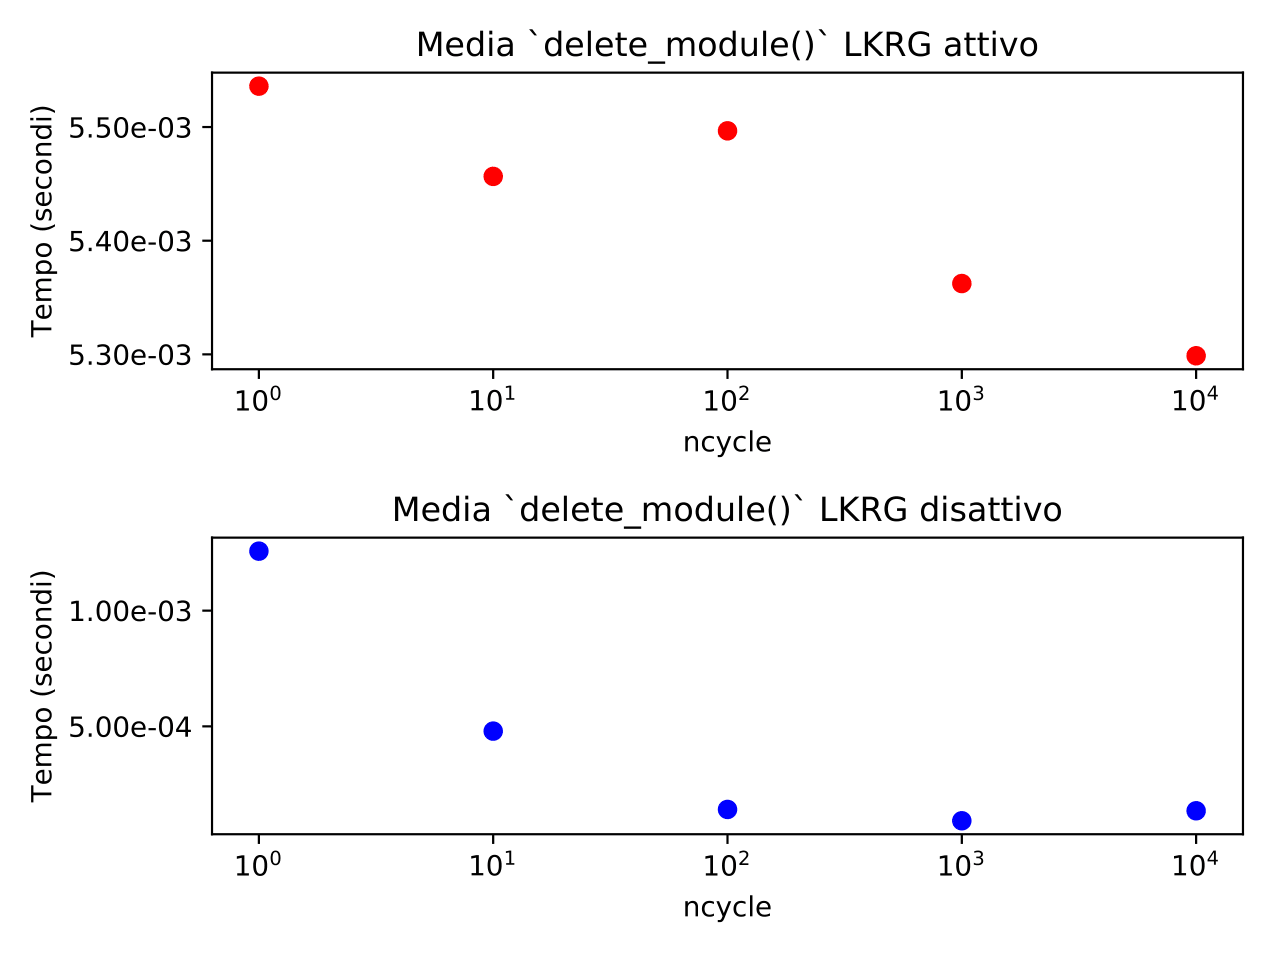
\includegraphics[scale=0.18]{Figures/Ubuntu/Mean1}
\caption[Media singole system call nei 5 benchmark parte 1 (Ubuntu)]{Media singole system call nei 5 benchmark parte 1 (Ubuntu).}
\label{fig:mean1UbuntuFig}
\end{figure}

\begin{figure}[!htbp]
\centering
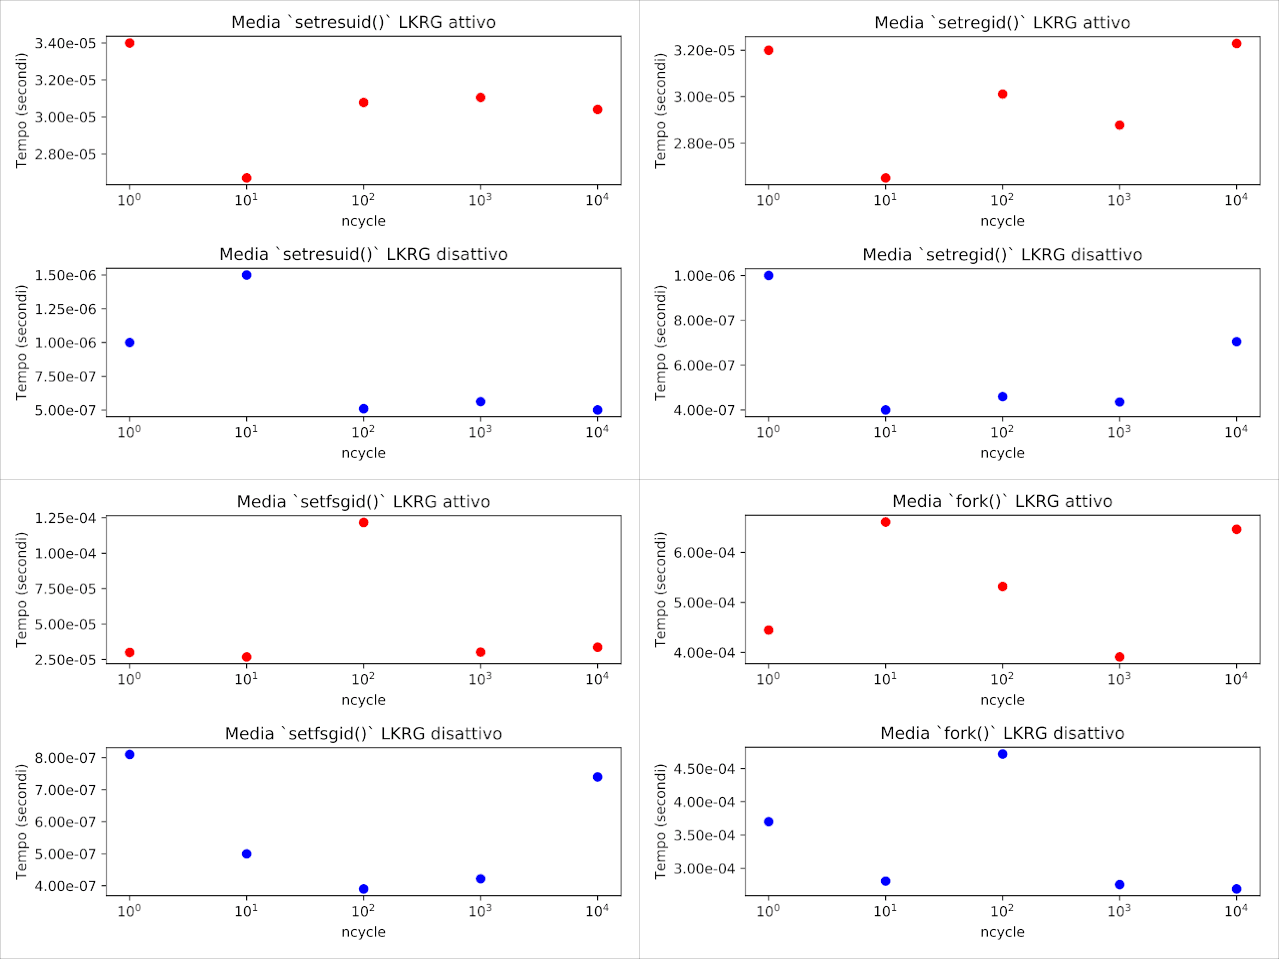
\includegraphics[scale=1.3]{Figures/Ubuntu/Mean2}
\caption[Media singole system call nei 5 benchmark parte 2 (Ubuntu)]{Media singole system call nei 5 benchmark parte 2 (Ubuntu).}
\label{fig:mean2UbuntuFig}
\end{figure}

\begin{figure}[!htbp]
\centering
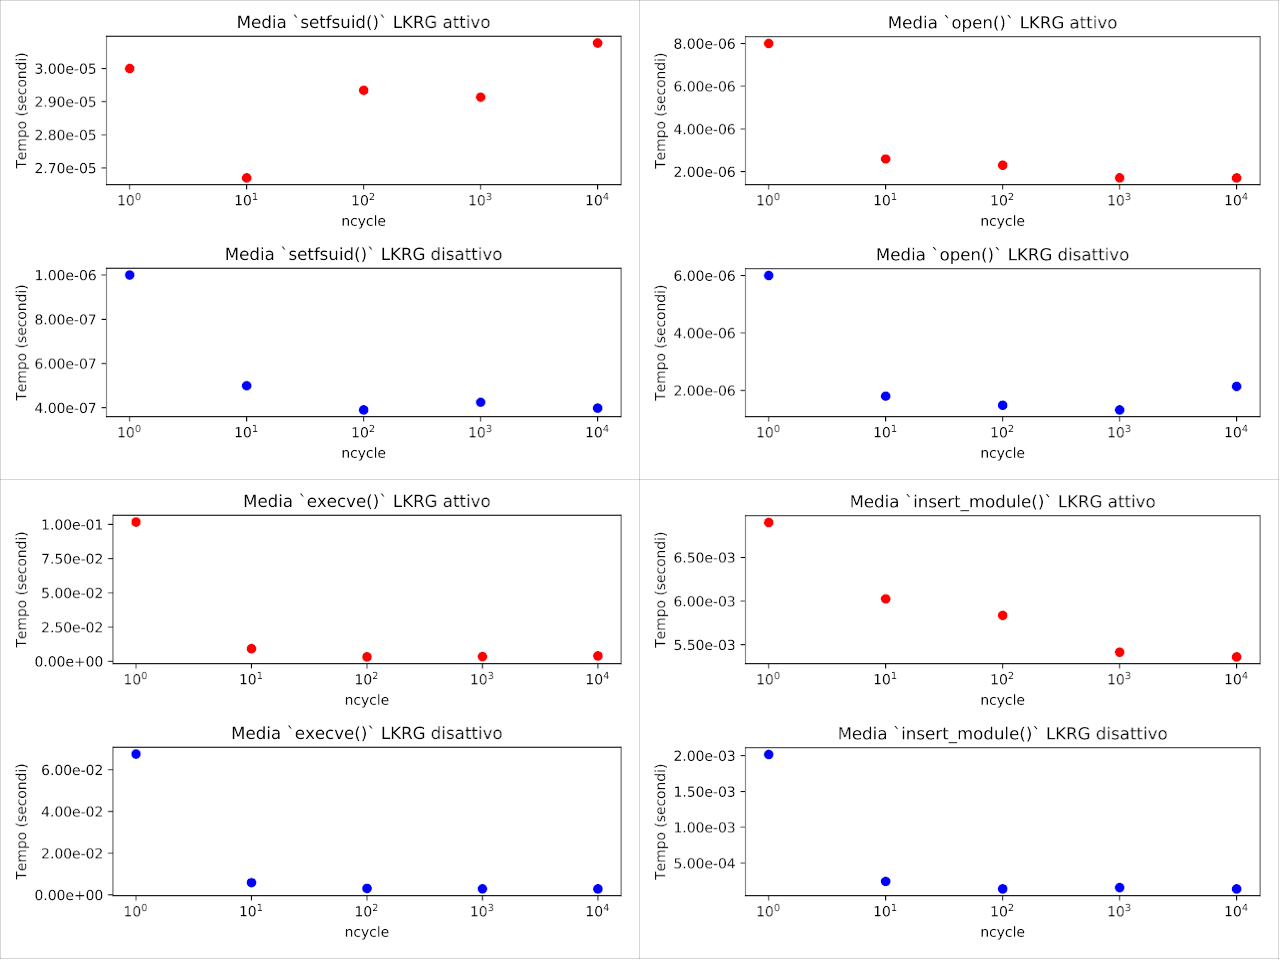
\includegraphics[scale=1.3]{Figures/Ubuntu/Mean3}
\caption[Media singole system call nei 5 benchmark parte 3 (Ubuntu)]{Media singole system call nei 5 benchmark parte 3 (Ubuntu).}
\label{fig:mean3UbuntuFig}
\end{figure}

\begin{figure}[!htbp]
\centering
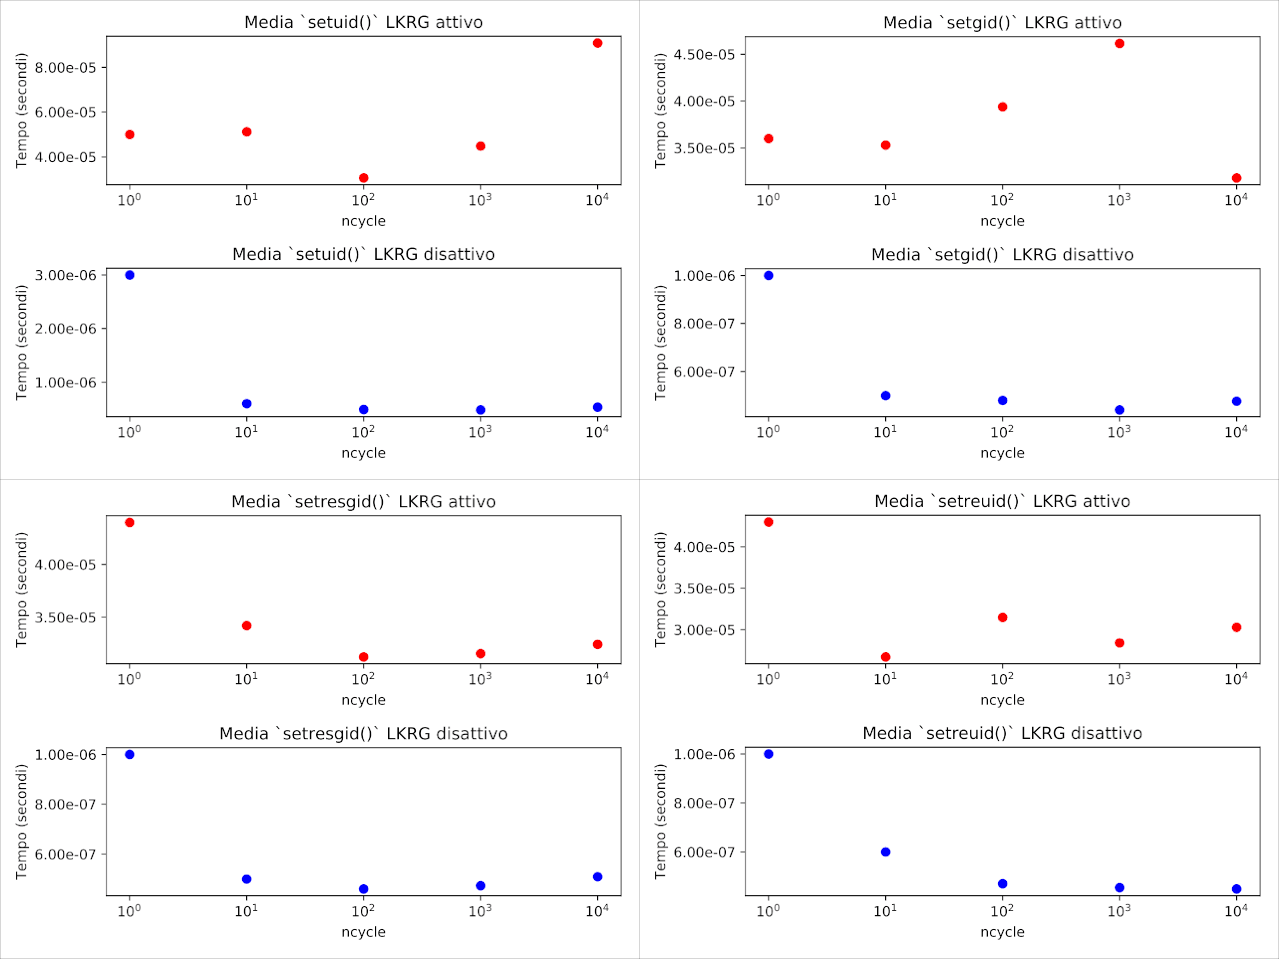
\includegraphics[scale=1.3]{Figures/Ubuntu/Mean4}
\caption[Media singole system call nei 5 benchmark parte 4 (Ubuntu)]{Media singole system call nei 5 benchmark parte 4 (Ubuntu).}
\label{fig:mean4UbuntuFig}
\end{figure}

Ad eccezione dei grafici in \autoref{fig:mean4UbuntuFig} che presentano valori oscillanti, nei restanti è chiaro l'intervento di un ottimizzatore, grazie al quale in base a quante chiamate vengono effettuate il tempo d'esecuzione medio della singola system call diminuisce in maniera esponenziale. Come scala per l'asse delle x è stata utilizzata una scala logaritmica per rappresentare il numero tutti i valori assunti da ncycle.

%----------------------------------------------------------------------------------------
%	DEBIAN TESTS
%----------------------------------------------------------------------------------------
\section{Test in Debian}

In questa sezione sono presentati i risultati della valutazione della seconda distribuzione presa in analisi: Debian. I test in questo ambiente, nonostante presentino varie similitudini con i risultati ottenuti in Ubuntu, suggeriscono un'ottima risposta del sistema al caricamento di LKRG.

Per seguire la stessa logica di presentazione della sezione precedente, iniziamo commentando i risultati ottenuti in seguito a 50 esecuzioni di SysBench con parametro ncycle=1 presentati nei seguenti grafici.

\begin{figure}[!ht]
\centering
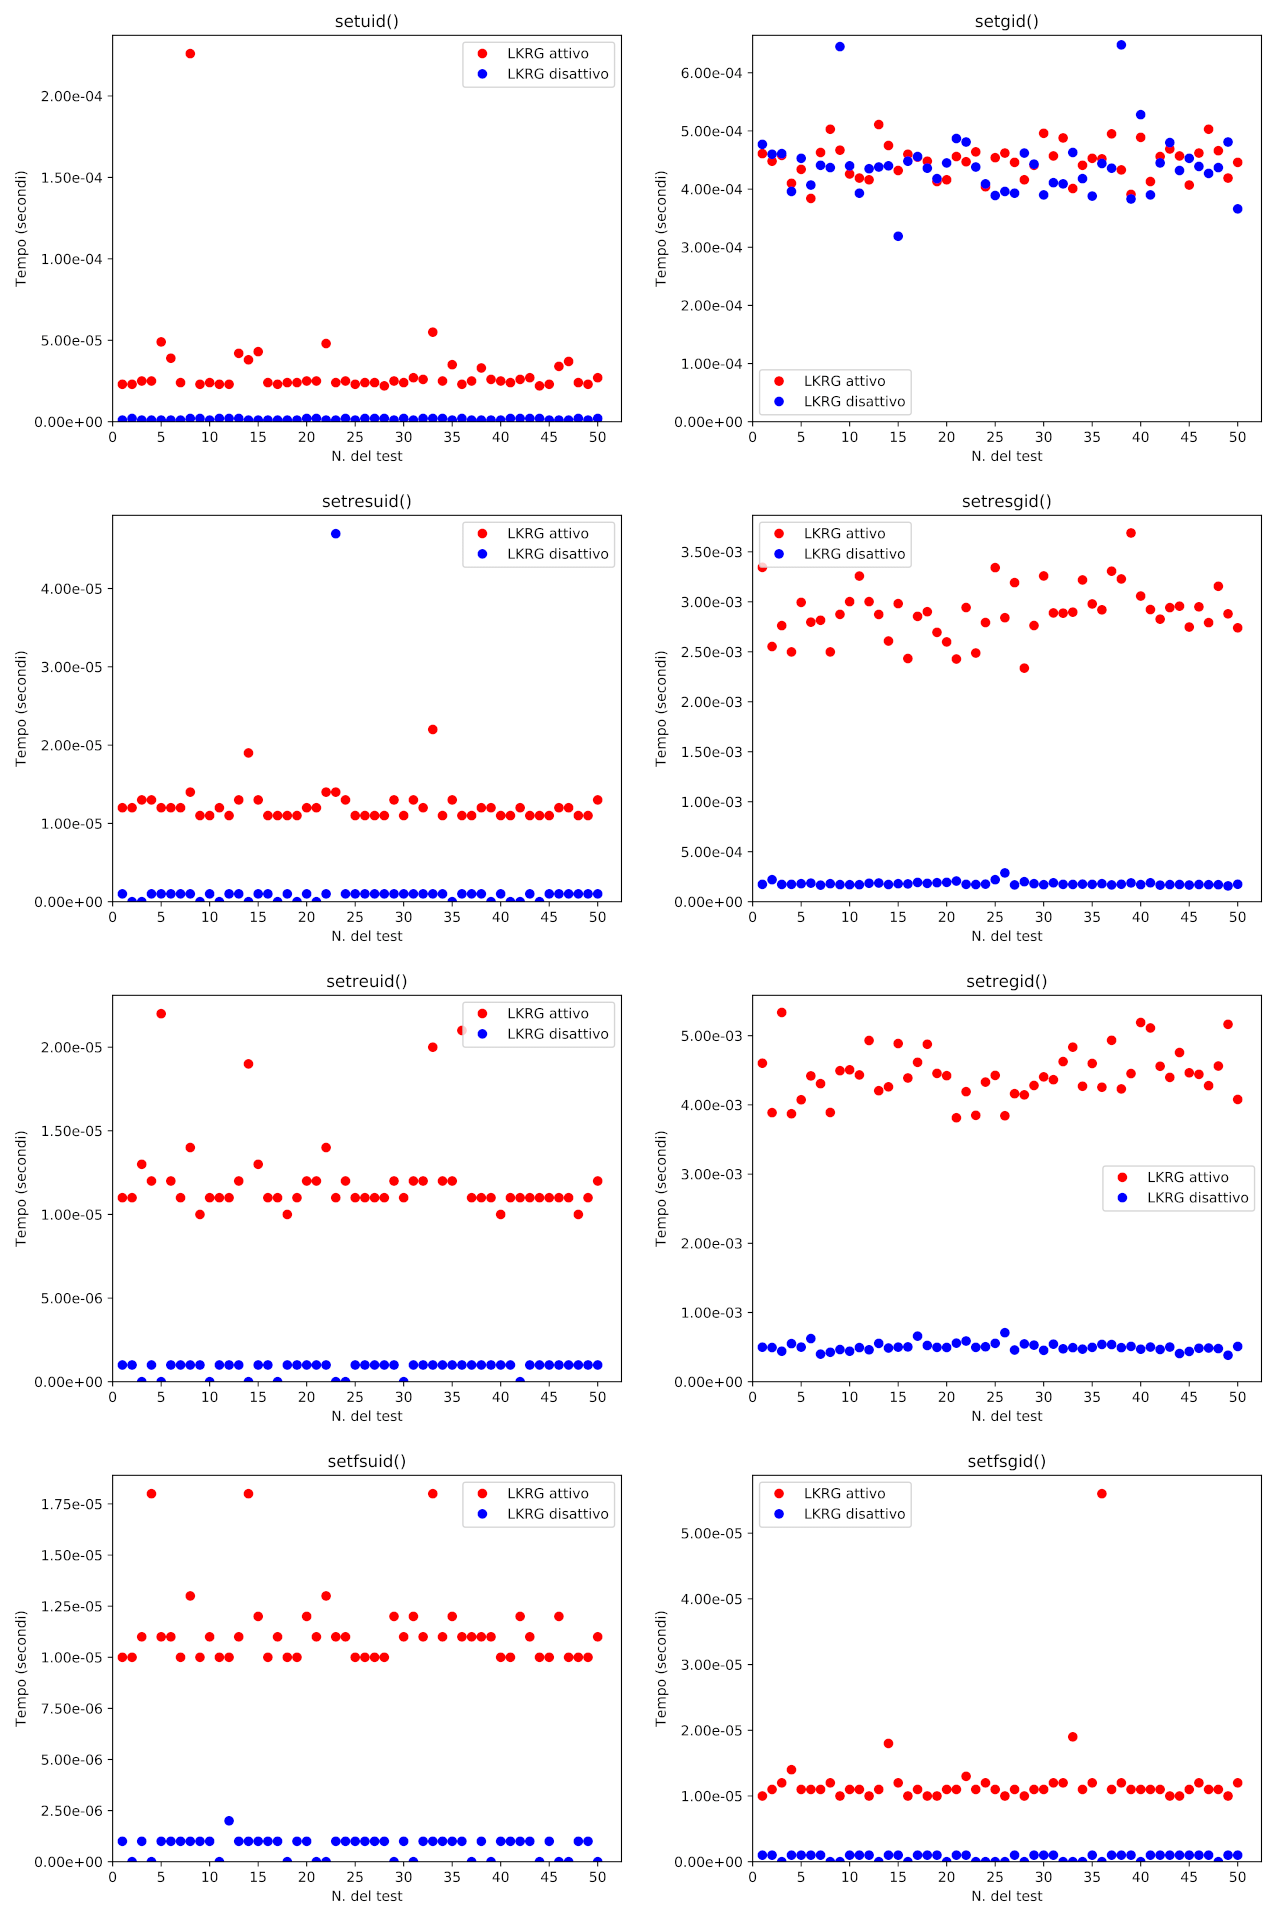
\includegraphics[scale=1.3]{Figures/Debian/SingleSet}
\caption[Benchmark funzioni \emph{setX} con ncycle=1 (Debian)]{Benchmark funzioni \emph{setX} con ncycle=1 (Debian).}
\label{fig:setxDebianFig}
\end{figure}

Come si può osservare in \autoref{fig:setxDebianFig} è chiara la differenza tra i tempi d'esecuzione delle varie system e l'overhead aggiunto da LKRG. Nonostante la dispersione dei grafici sia simile a quelli presentati per Ubuntu, cambia il range dei tempi d'esecuzione: ad esempio per la \emph{setresgid()} osserviamo che i tempi misurati senza il modulo attivo sono di due ordini di grandezza più piccoli rispetto a quelli con LKRG presente, mentre in Ubuntu la differenza è minima, cambia solamente un fattore di proporzionalità pari a 3.
La system call che risulta essere meno influenzata anche in ambiente Debian risulta essere la \emph{setgid()}, i cui valori oscillano in un intorno di $1x10^{-4}$ che rispetto ai tempi misurati è relativamente piccolo. Esclusa questa system call e la \emph{setresuid()}, i cui test rivelano qualche rallentamento nell'esecuzione della funzione anche senza LKRG, nei grafici di tutte le altre funzionalità si osserva che mentre in presenza del modulo i tempi campionati sono molto più variabili e dispersi, in sua assenza i valori risultano essere più omogenei ed allineati, sebbene vi sia qualche differenza ma in grandezza minore.

\begin{table}[!htbp]
\centering
\begin{tabular}{|c|c|c|c|c|}
\hline
\textbf{SystemCall} & \bm{$\overline{x}$} \textbf{loaded} & \bm{$\overline{x}$} \textbf{unloaded} & \bm{$\sigma$} \textbf{loaded} & \bm{$\sigma$} \textbf{unloaded}\\
\hline
setuid() & 3.202e-05 & 1.460e-06 & 2.877e-05 & 4.984e-07 \\
\hline
setgid() & 4.477e-04 & 4.402e-04 & 2.982e-05 & 5.500e-05 \\
\hline
setresuid() & 1.220e-05 & 1.660e-06 & 1.949e-06 & 6.492e-06 \\
\hline
setresgid() & 2.894e-03 & 1.812e-04 & 2.685e-04 & 1.971e-05 \\
\hline
setreuid() & 1.212e-05 & 8.200e-07 & 2.628e-06 & 3.842e-07 \\
\hline
setregid() & 4.438e-03 & 5.018e-04 & 3.587e-04 & 5.863e-05 \\
\hline
setfsuid() & 1.124e-05 & 7.400e-07 & 1.893e-06 & 4.821e-07 \\
\hline
setfsgid() & 1.228e-05 & 6.600e-07 & 6.465e-06 & 4.737e-07 \\
\hline
\end{tabular}
\caption{Dati benchmark funzioni \emph{setX} con ncycle=1 (Debian)}
\label{table:setxDebianData}
\end{table}

Dalla \autoref{table:setxDebianData} si evince quanto appena commentato: concentrandosi sulla deviazione standard in entrambe le situazioni, confermiamo appunto che i valori sono più concentrati ed omogenei quando LKRG non è presente nel sistema, mentre una volta caricato i tempi misurati variano in maniera più evidente. Si può affermare dunque che i controlli d'integrità, sebbene non comportino un aumento eccessivo della chiamata, influenzino in maniera variabile l'esecuzione. Per fare un esempio si considerino i dati relativi alla \emph{setuid()}: una deviazione standard di $2.877x10^{-5}$ con LKRG presente è accettabile rispetto alla media $3.202x10^{-5}$ delle chiamate, ma se la si confronta con i valori misurati in assenza del modulo risulta essere non trascurabile, in quanto la deviazione è dell'ordine del $10^{-7}$. È necessario prima di giungere a conclusioni considerare questi fattori e queste differenze negli ordini di grandezza dei dati, in modo da comprendere e confrontare con coerenza la variazione dei tempi d'esecuzione delle funzioni.
\\\par

\begin{figure}[!ht]
\centering
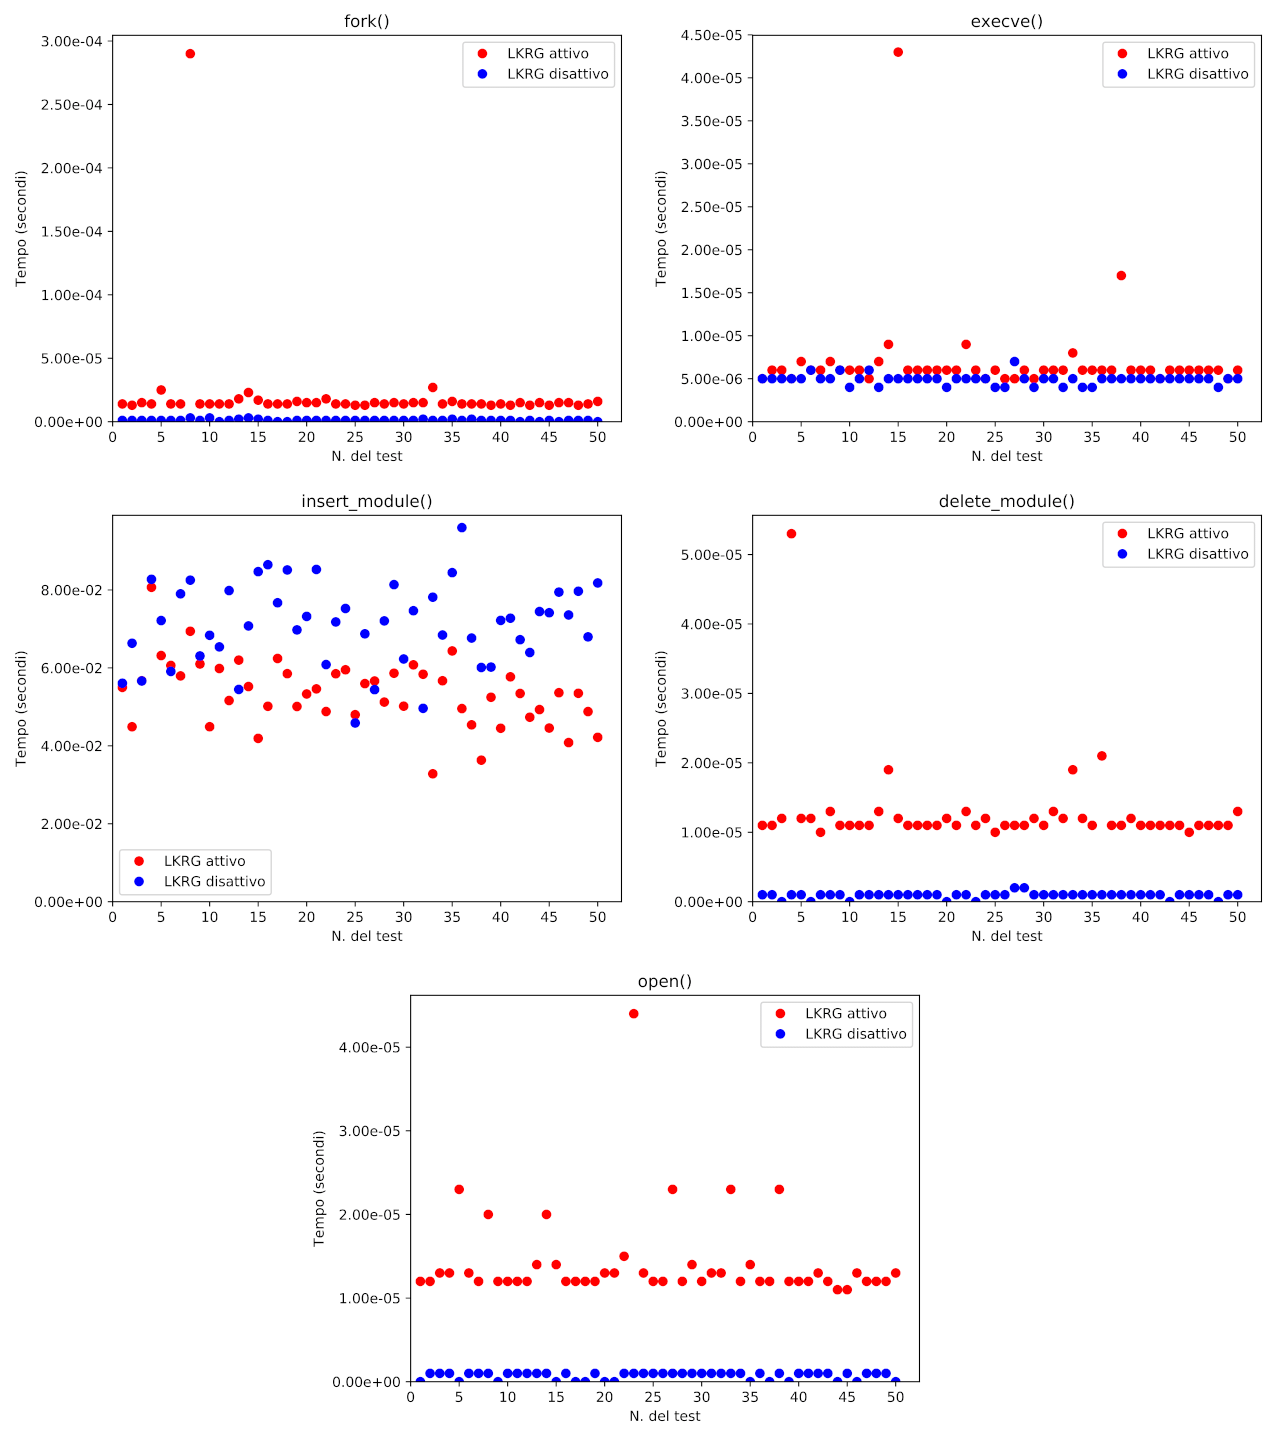
\includegraphics[scale=1.4]{Figures/Debian/SingleOthers}
\caption[Benchmark restanti funzioni con ncycle=1 (Debian)]{Benchmark restanti funzioni con ncycle=1 (Debian).}
\label{fig:othersDebianFig}
\end{figure}

Sorprendentemente, il grafico della \emph{execve()} in \autoref{fig:othersDebianFig} rivela che il tempo d'esecuzione è minore quando misurato con il modulo presente, mentre risulta essere leggermente maggiore nel caso opposto, inducendo a concludere che tale system call non sia influenzata da LKRG. La scala dei valori in tale grafico risulta essere meno estesa, suggerendo dunque più omogeneità nei dati rispetto agli altri dove si può osservare che in ogni test delle funzionalità vi è sempre qualche valore che si discosta maggiormente dalla media. Ad esempio si consideri la \emph{fork()}: una misurazione è risultata essere di un'ordine di grandezza e mezzo più grande rispetto a tutte le altre, probabilmente dovuto a qualche ritardo nell'allocazione di risorse per il processo figlio da parte del programma e non a causa di LKRG. Ancora una volta si assiste ad un aumento di due ordini di grandezza del tempo d'esecuzione della \emph{open()} che, come in Ubuntu, varia da $7.200e^{-07}$ in assenza del modulo a $1.424e^{-05}$ una volta caricato.

\begin{table}[!htbp]
\centering
\begin{tabular}{|c|c|c|c|c|}
\hline
\textbf{SystemCall} & \bm{$\overline{x}$} \textbf{loaded} & \bm{$\overline{x}$} \textbf{unloaded} & \bm{$\sigma$} \textbf{loaded} & \bm{$\sigma$} \textbf{unloaded}\\
\hline
open() & 1.424e-05 & 7.200e-07 & 5.335e-06 & 4.490e-07 \\
\hline
fork() & 2.058e-05 & 1.080e-06 & 3.859e-05 & 6.882e-07 \\
\hline
execve() & 7.000e-06 & 4.900e-06 & 5.430e-06 & 5.745e-07 \\
\hline
insert\_module() & 5.349e-02 & 7.114e-02 & 8.344e-03 & 1.041e-02 \\
\hline
delete\_module() & 1.270e-05 & 9.000e-07 & 6.133e-06 & 4.123e-07 \\
\hline
\end{tabular}
\caption{Dati benchmark restanti funzioni con ncycle=1 (Debian)}
\label{table:othersDebianData}
\end{table}

\clearpage

Nella tabella \autoref{table:othersDebianData} si osservi come le system call \emph{open()} e \emph{delete\_module()} siano quelle più influenzate dal modulo, in quanto i valori medi si innalzano di fattore 1000, passando da tempi come $7.200e^{-07}$ e $9.000e-07$ a $1.424e-05$ e $1.270e-05$. Coerentemente con quanto detto in prececenza, non solo la media della singola chiamata alla funzione \emph{execve()} risulta essere leggermente maggiore in assenza del modulo, ma anche la deviazione standard (10 volte minore).
\\\par

\begin{figure}[!ht]
\centering
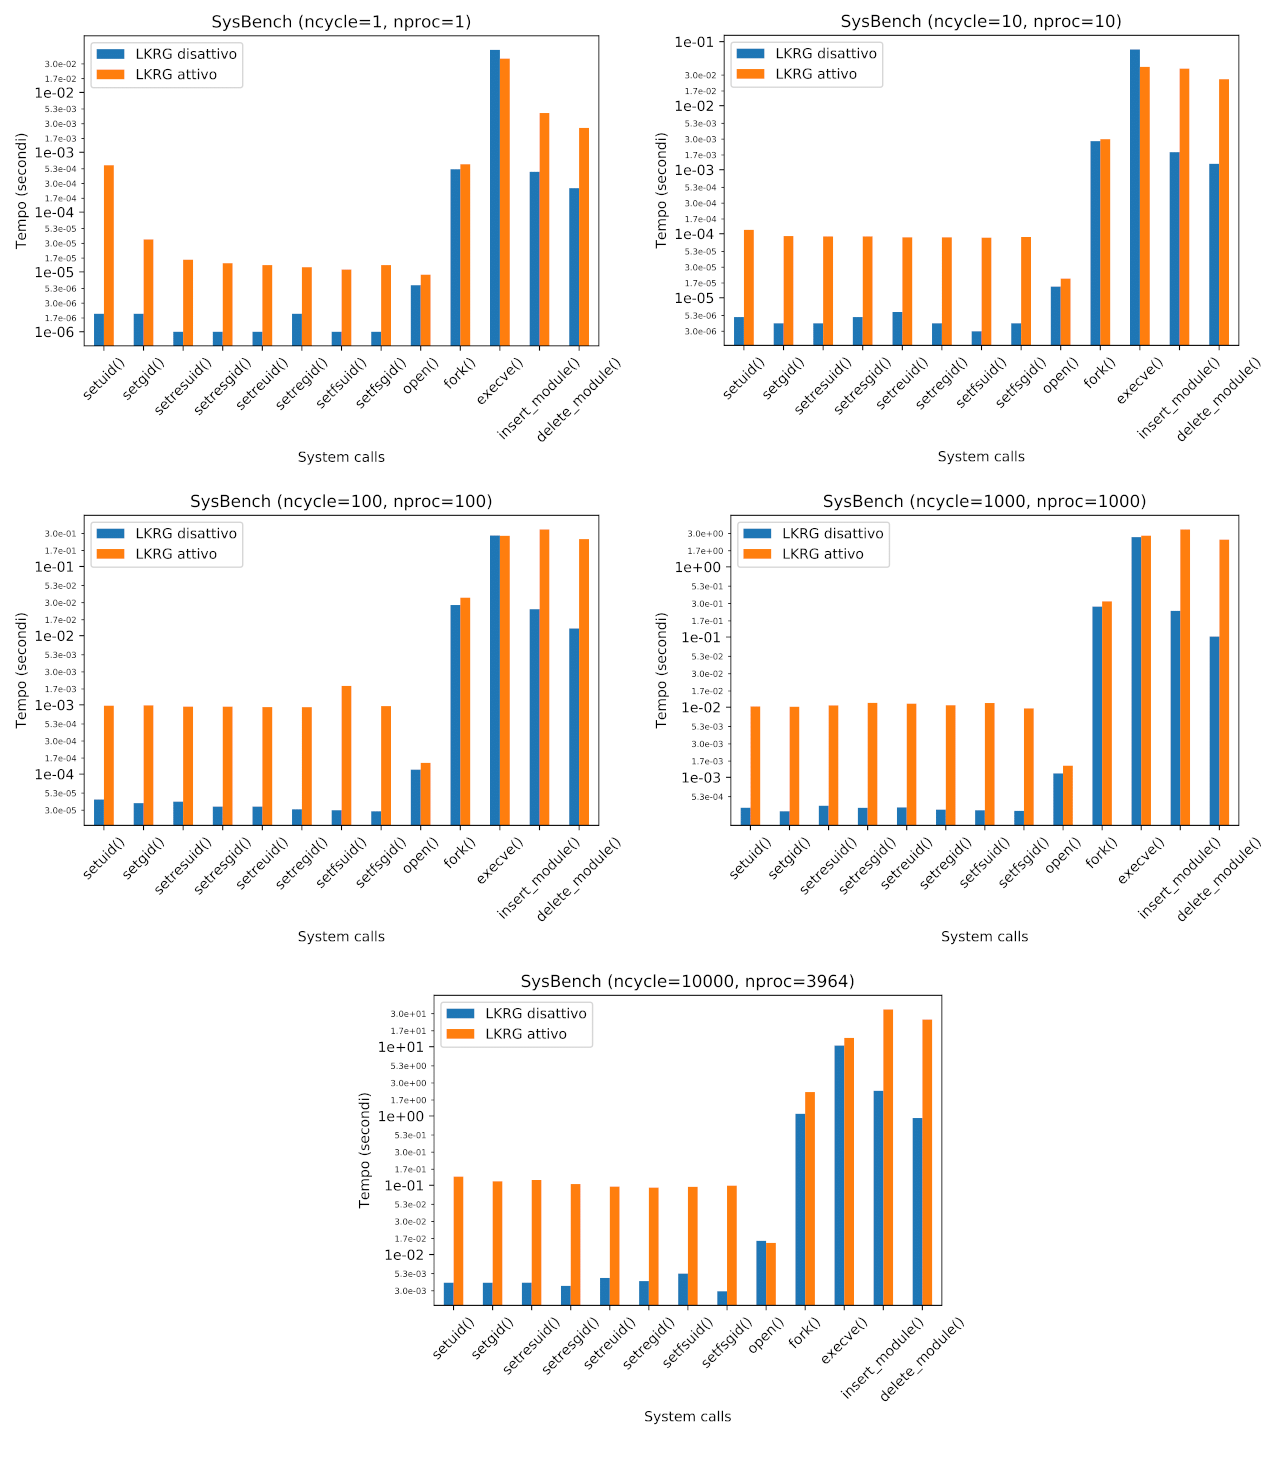
\includegraphics[scale=1.4]{Figures/Debian/Total}
\caption[Benchmark tempo totale (Debian)]{Benchmark tempo totale (Debian).}
\label{fig:totDebianFig}
\end{figure}

Procediamo ora con la medesima analisi effettuata in Ubuntu, ovvero il tempo d'esecuzione della singola system call nel caso venisse richiamata più volte all'interno del programma. Il test è stato effettuato ugualmente, con ncycle che assume i valori 1, 10, 100, 1000 e 10000 ed il sistema che si trova nello stesso stato in cui era la macchina Ubuntu. L'obiettivo è sempre quello di osservare il tempo medio d'esecuzione della singola system call per dedurre se anche in questo sistema vengono apportate ottimizzazioni.

In \autoref{fig:totDebianFig} si osserva il tempo totale d'esecuzione delle system call nei 5 scenari con ncycle differente. Iniziando a valutare il test con ncycle=1 che rappresenta inoltre i test discussi fino ad ora, si nota come LKRG influenzi maggiormente le funzioni \emph{setX()} e quelle inerenti alle operazioni con i moduli, le quali variano maggiormente rispetto alla \emph{open()}, \emph{fork() e la \emph{execve()}}. Quest'ultima soprattutto presenta tempi d'esecuzione maggiori in assenza del modulo nei test in cui viene richiamata un numero relativamente piccolo di volte, mentre più cresce ncycle più i due tempi tendono a differire per veramente poche unità sembrando quasi pareggianti. Vi è una lieve differenza anche nelle altre due funzionalità, le quali però mantengono il rapporto $\frac{Tattivo}{Tdisattivo}$ quasi costante. Sicuramente l'utente lanciando il programma è in grado di percepire la differenza d'esecuzione della \emph{insert\_module()} e \emph{delete\_module()}, in quanto in ordini di grandezza sono quelle con la differenza più alta (persino 30 volte più alta nei test con ncycle=10000), ma quelle che in percentuale al loro tempo d'esecuzione in assenza del modulo hanno subito maggiori rallentamenti sono le \emph{setX()} come già commentato.

\begin{table}[!htbp]
\centering
\begin{tabular}{|c|c|c|c|c|}
\hline
\textbf{SystemCall} & \bm{$\overline{x}$} \textbf{loaded} & \bm{$\overline{x}$} \textbf{unloaded} & \bm{$\sigma$} \textbf{loaded} & \bm{$\sigma$} \textbf{unloaded}\\
\hline
setuid() & 1.304e-04 & 7.380e-07 & 2.383e-04 & 6.326e-07 \\
\hline
setgid() & 1.512e-05 & 7.000e-07 & 9.966e-06 & 6.505e-07 \\
\hline
setresuid() & 1.142e-05 & 5.171e-07 & 2.494e-06 & 2.415e-07 \\
\hline
setresgid() & 1.089e-05 & 5.119e-07 & 1.766e-06 & 2.507e-07 \\
\hline
setreuid() & 1.038e-05 & 5.544e-07 & 1.544e-06 & 2.403e-07 \\
\hline
setregid() & 9.999e-06 & 6.941e-07 & 1.179e-06 & 6.540e-07 \\
\hline
setfsuid() & 1.188e-05 & 4.941e-07 & 3.586e-06 & 2.671e-07 \\
\hline
setfsgid() & 1.020e-05 & 4.634e-07 & 1.438e-06 & 2.712e-07 \\
\hline
open() & 3.077e-06 & 2.274e-06 & 2.969e-06 & 1.871e-06 \\
\hline
fork() & 4.332e-04 & 3.241e-04 & 1.349e-04 & 9.801e-05 \\
\hline
execve() & 9.963e-03 & 1.340e-02 & 1.345e-02 & 1.906e-02 \\
\hline
insert\_module() & 3.727e-03 & 2.734e-04 & 4.233e-04 & 1.006e-04 \\
\hline
delete\_module() & 2.510e-03 & 1.394e-04 & 5.203e-05 & 5.722e-05 \\
\hline
\end{tabular}
\caption{Dati benchmark con ncycle=1, 10, 100, 1000, 10000 (Debian)}
\label{table:totDebianData}
\end{table}

Tralasciando la precisione dei valori, l'analisi da effettuare è la medesima di quella inerente al sistema Ubuntu, ovvero da questa tabella si osservano valori che porterebbero a pensare ad un errore di misurazione. In realtà, osservando i grafici sottostanti si osserva come il tempo d'esecuzione medio delle singole system call diminuisca all'aumentare del numero di volte che vengono testate.

\clearpage

\begin{figure}[!htbp]
\centering
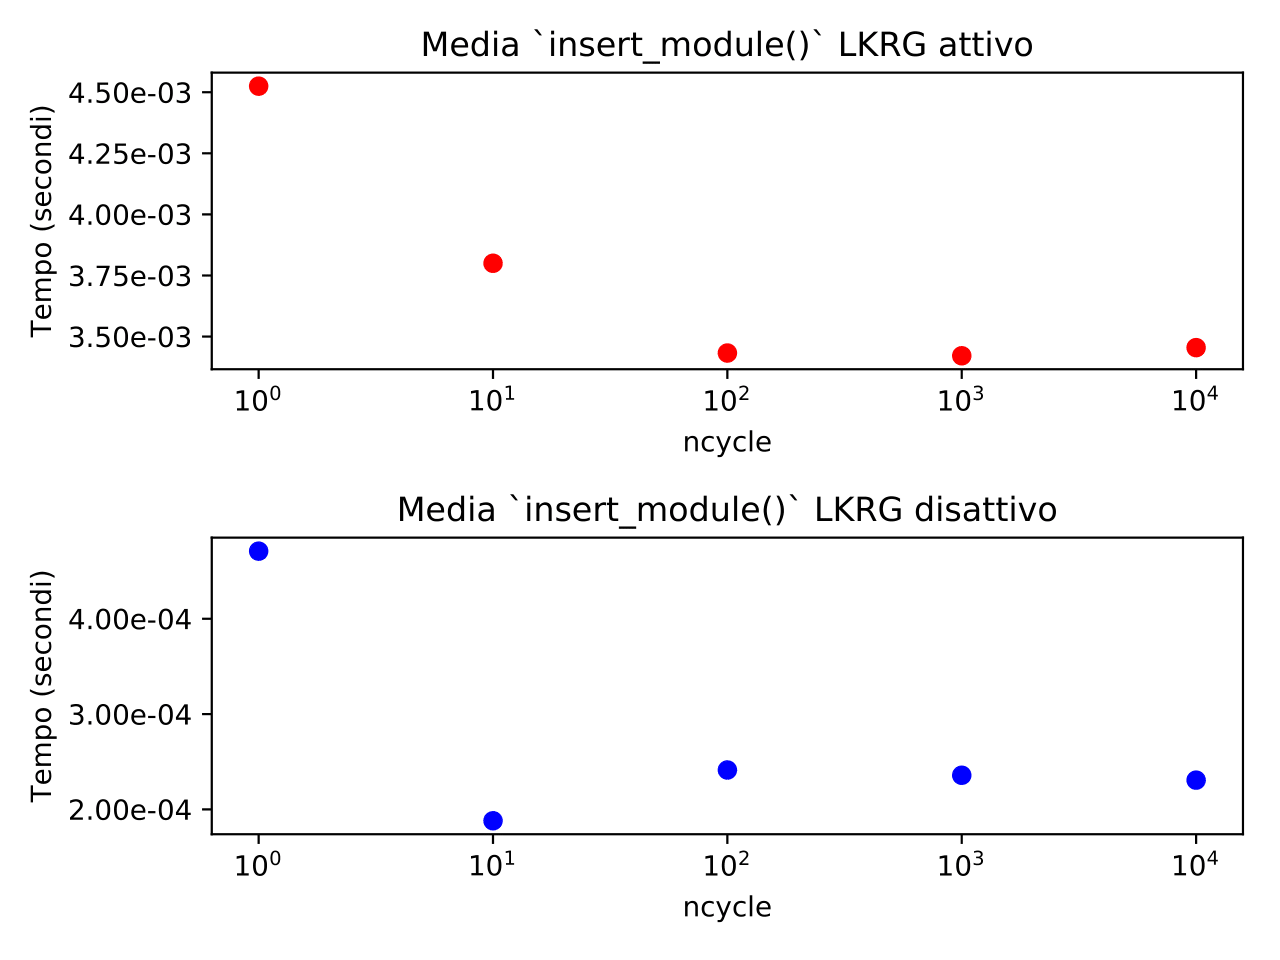
\includegraphics[scale=0.22]{Figures/Debian/Mean1}
\caption[Media singole system call nei 5 benchmark parte 1 (Debian)]{Media singole system call nei 5 benchmark parte 1 (Debian).}
\label{fig:mean1DebianFig}
\end{figure}

\begin{figure}[!htbp]
\centering
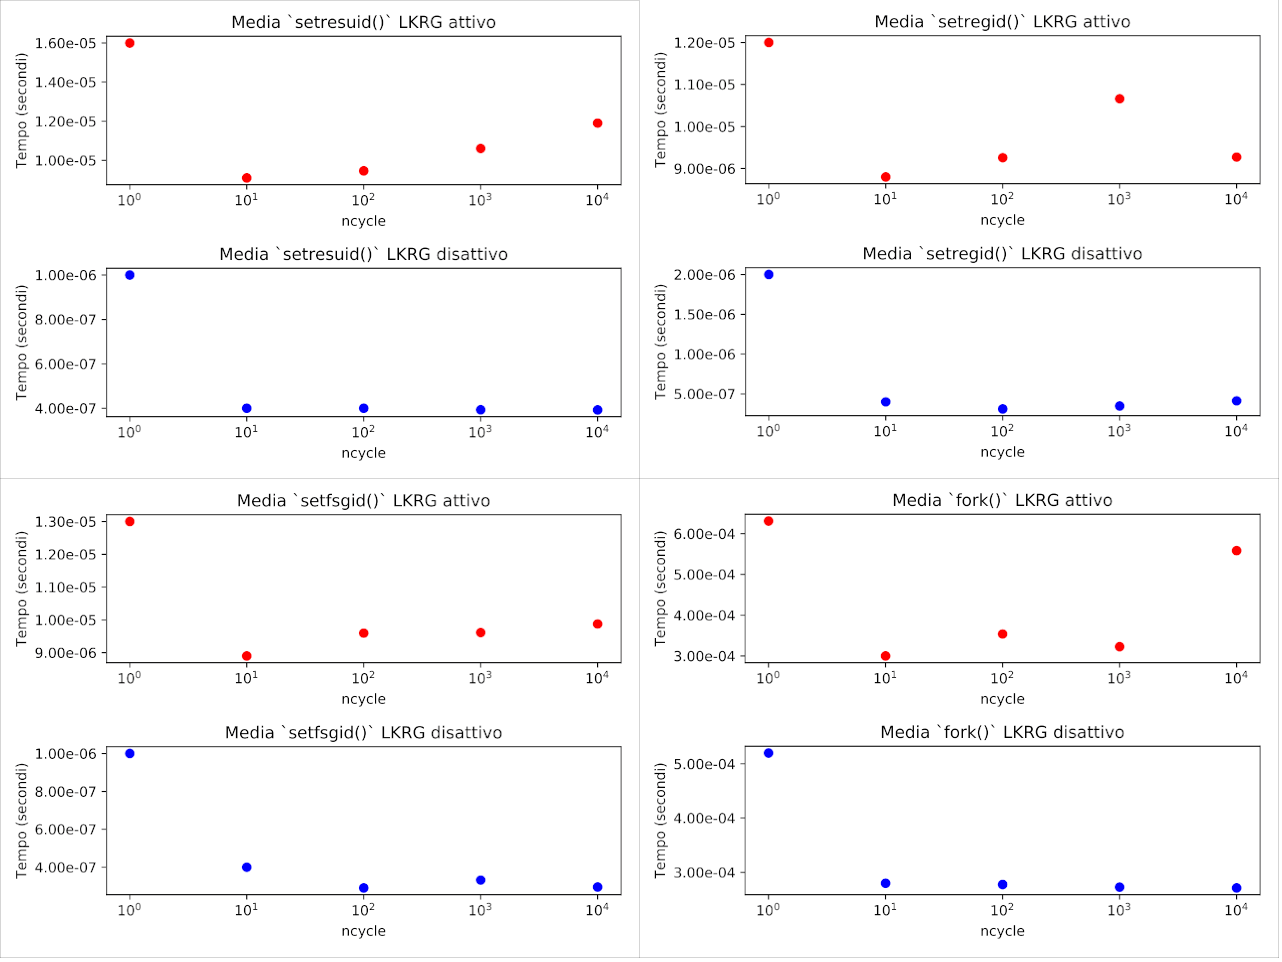
\includegraphics[scale=1.4]{Figures/Debian/Mean2}
\caption[Media singole system call nei 5 benchmark parte 2 (Debian)]{Media singole system call nei 5 benchmark parte 2 (Debian).}
\label{fig:mean2DebianFig}
\end{figure}

\clearpage

\begin{figure}[!htbp]
\centering
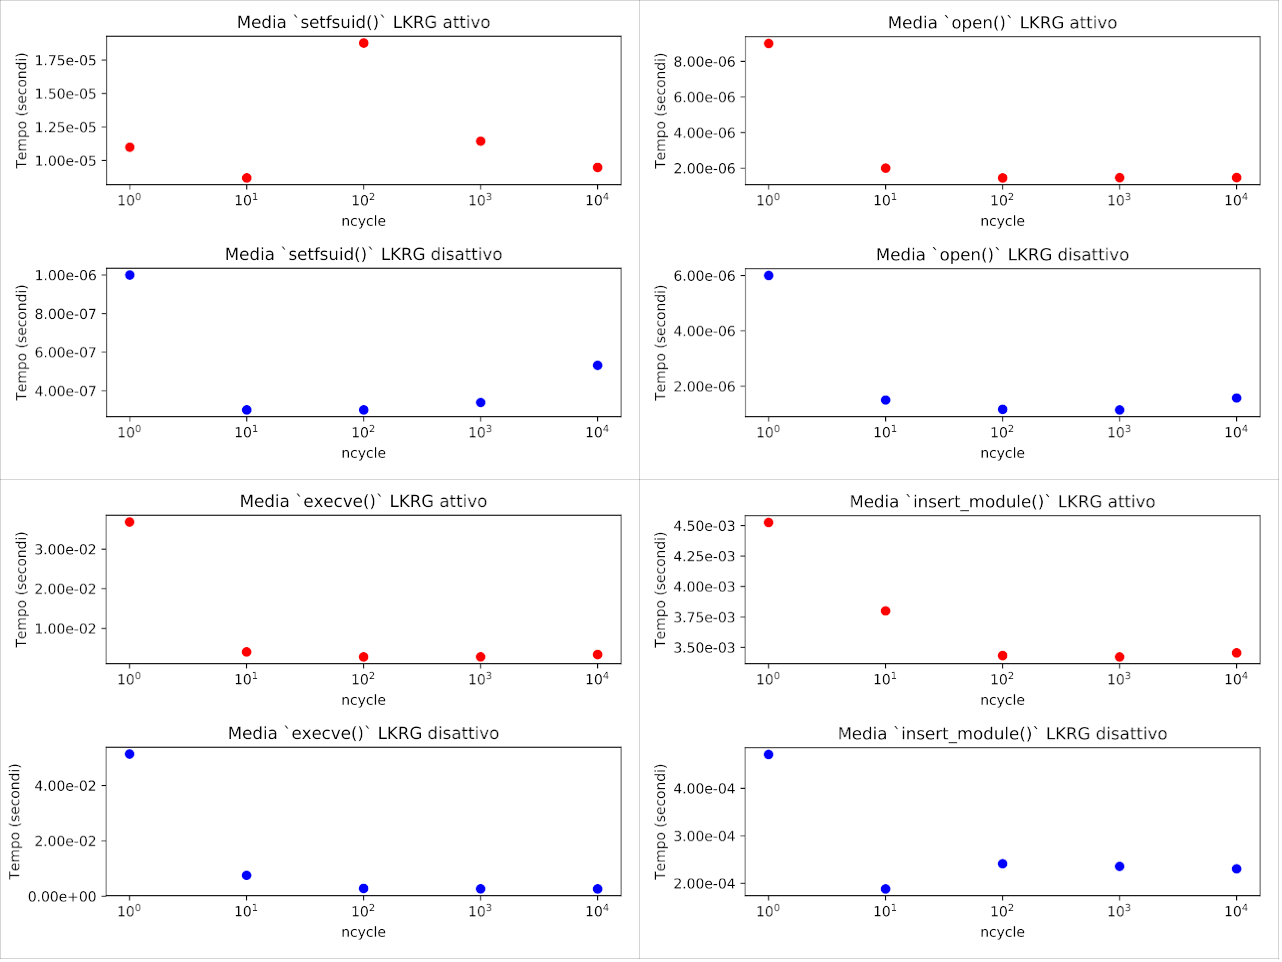
\includegraphics[scale=1.3]{Figures/Debian/Mean3}
\caption[Media singole system call nei 5 benchmark parte 3 (Debian)]{Media singole system call nei 5 benchmark parte 3 (Debian).}
\label{fig:mean3DebianFig}
\end{figure}

\begin{figure}[!htbp]
\centering
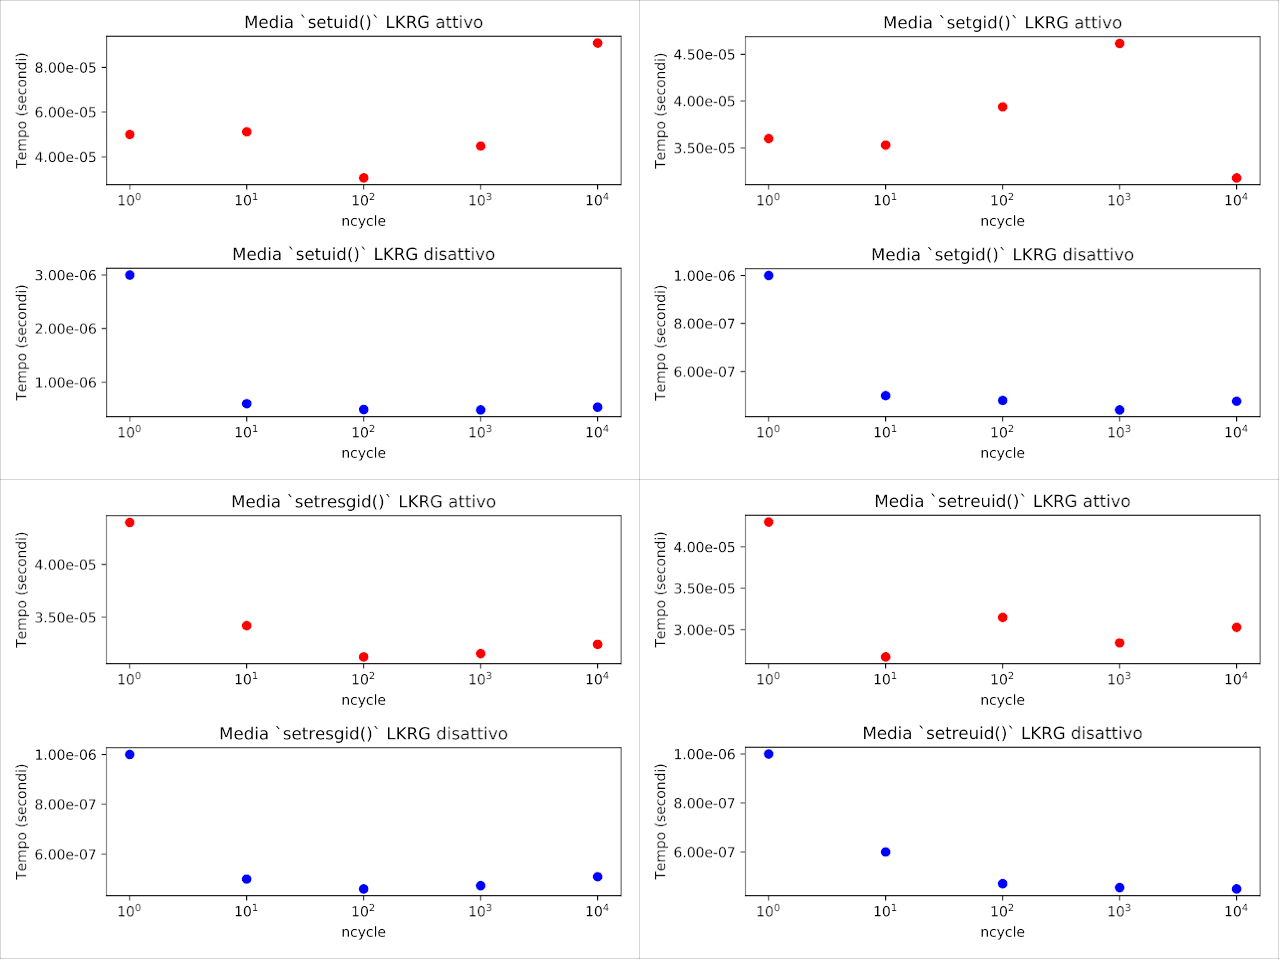
\includegraphics[scale=1.3]{Figures/Debian/Mean4}
\caption[Media singole system call nei 5 benchmark parte 4 (Debian)]{Media singole system call nei 5 benchmark parte 4 (Debian).}
\label{fig:mean4DebianFig}
\end{figure}

Nei grafici rappresentati in queste quattro figure è immediato notare l'andamento esponenziale dei tempi delle singole chiamate di sistema quando il modulo non è attivo. A differenza dei tempi misurati in Ubuntu, questi valori sono più stabili e la curva esponenziale che formano è ancora più evidente e precisa. I valori misurati con LKRG caricato nel kernel rimangono invece abbastanza instabili per la maggior parte delle system call, mentre per altre come la \emph{open()} mantengono un andamento esponenziale simile a quelli misurati in assenza del modulo, sebbene siano leggermente più elevati.

%----------------------------------------------------------------------------------------
%	MINT TESTS
%----------------------------------------------------------------------------------------
\section{Test in Mint}

L'ultimo sistema da testare, nonchè uno tra i più conosciuti ed utilizzati, è Linux Mint. I test hanno rilevato un comportamento differente del sistema, i cui risultati talvolta convergono a quelli ottenuti in Ubuntu, mentre per certe system call sono intermedi tra quelli di Ubuntu e Debian.

In \autoref{fig:setxMintFig} sono riportati i grafici ottenuti mediante la solita esecuzione di SysBench con ncycle=1, come per le altre valutazioni.

Il primo commento in merito ai grafici riguarda il comportamento della funzione \emph{setgid()}: il tempo d'esecuzione di tale funzione, escluso qualche test eccezionale, non varia in maniera clamorosa tra la misurazione con LKRG e senza. Inoltre, anche la \emph{setuid()} e molte altre di queste funzioni presentano risultati più analoghi, sebbene leggermente differenti ma di un fattore irrilevante, a quelli ottenuti in Debian rispetto a quelli in Ubuntu, nei quali vi era più di un test fuori dalla media.
Per altre system call come la \emph{setregid()} e la \emph{setfsuid()} si può affermare l'opposto. La distribuzione dei grafici risulta essere abbastanza chiara come negli altri sistemi, facilitando la lettura e indicando in maniera chiara l'overhead causato da LKRG; si osservi che a seconda della system call il fattore di differenza tra i tempi d'esecuzione è circa 1.5, 3, 10 o 100.

\begin{table}[!htbp]
\centering
\begin{tabular}{|c|c|c|c|c|}
\hline
\textbf{SystemCall} & \bm{$\overline{x}$} \textbf{loaded} & \bm{$\overline{x}$} \textbf{unloaded} & \bm{$\sigma$} \textbf{loaded} & \bm{$\sigma$} \textbf{unloaded}\\
\hline
setuid() & 3.862e-05 & 2.060e-06 & 1.062e-05 & 4.200e-07 \\
\hline
setgid() & 4.658e-04 & 3.863e-04 & 1.436e-04 & 5.517e-05 \\
\hline
setresuid() & 3.212e-05 & 1.380e-06 & 4.325e-06 & 4.854e-07 \\
\hline
setresgid() & 3.843e-03 & 1.052e-03 & 3.305e-04 & 8.837e-05 \\
\hline
setreuid() & 2.392e-05 & 1.120e-06 & 1.707e-06 & 1.608e-06 \\
\hline
setregid() & 4.811e-03 & 1.473e-03 & 3.432e-04 & 1.055e-04 \\
\hline
setfsuid() & 2.276e-05 & 6.800e-07 & 1.871e-06 & 4.665e-07 \\
\hline
setfsgid() & 2.278e-05 & 4.800e-07 & 3.402e-06 & 4.996e-07 \\
\hline
\end{tabular}
\caption{Dati benchmark funzioni \emph{setX()} con ncycle=1 (Mint)}
\label{table:setxMintData}
\end{table}

Nella tabella \autoref{table:setxMintData} si noti come la deviazione standard dei valori quando il modulo è attivo sia sempre maggiore rispetto a quella calcolata in sua assenza. Ugualmente, anche la media delle singole chiamate è sempre minore, talvolta persino 100 volte più piccola se prendiamo in considerazione la \emph{setfsuid()} e la \emph{setfsgid()}. 

\clearpage

\begin{figure}[!ht]
\centering
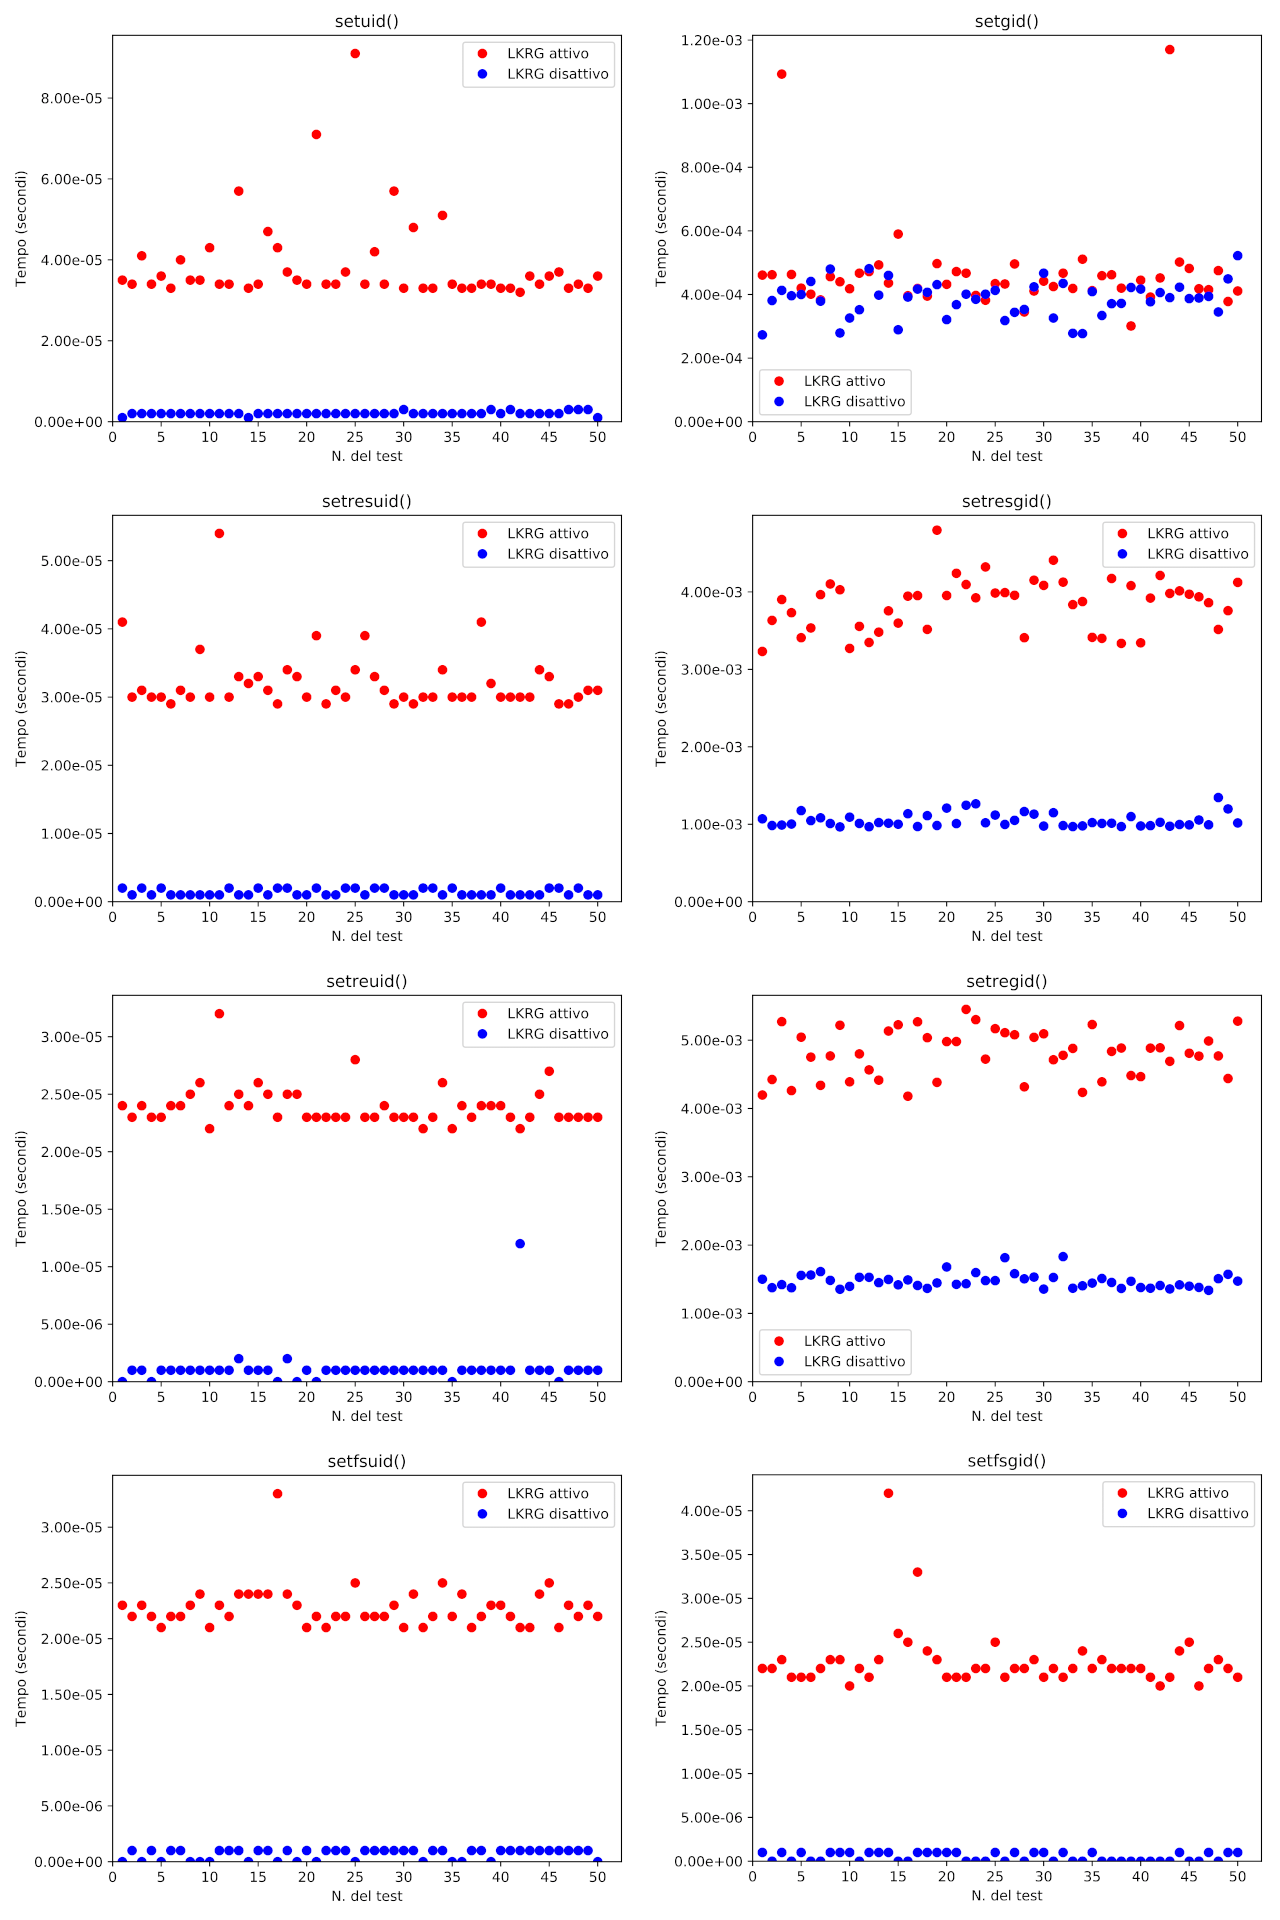
\includegraphics[scale=1.35]{Figures/Mint/SingleSet}
\caption[Benchmark funzioni \emph{setX} con ncycle=1 (Mint)]{Benchmark funzioni \emph{setX} con ncycle=1 (Mint).}
\label{fig:setxMintFig}
\end{figure}

Si può dedurre che il sovraccarico di istruzioni aggiunte da LKRG non sia trascurabile se ci atteniamo a considerare i risultati all'interno del loro ordine di grandezza. Infatti, la maggior parte delle funzionalità nella tabella hanno dei tempi molto differenti.


I risultati delle system call raffigurate in figura \autoref{fig:othersMintFig} si avvicinano maggiormente a quelli ottenuti in Ubuntu rispetto a Debian, ad esclusione della \emph{insert\_module()}; quest'ultima ha un comportamento interessante anche in Mint, dato che i valori massimi sono registrati quando nel sistema non vi è LKRG. Per quanto riguarda le altre funzionalità, esse hanno un andamento stabile come si può osservare dai grafici: i valori ottenuti in assenza del modulo sono abbastanza omogenei tra loro con poche misurazioni isolate, e lo stesso vale per gli altri.

\begin{figure}[!ht]
\centering
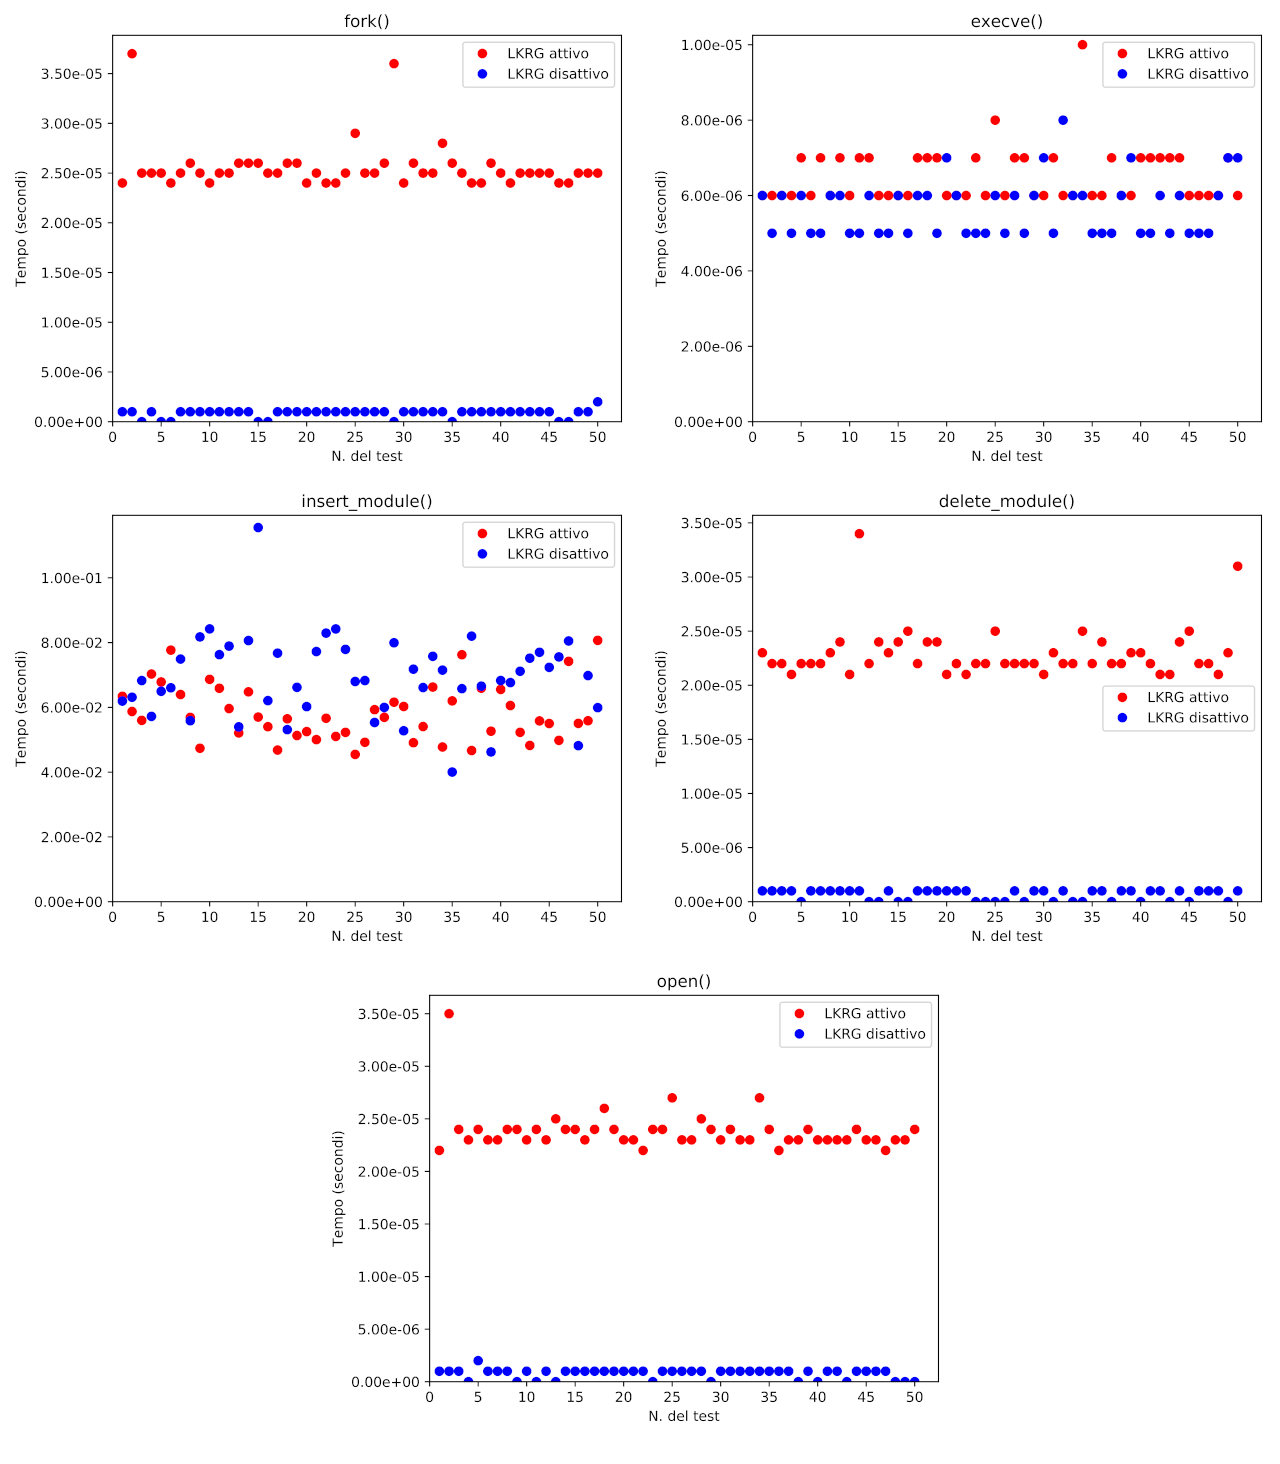
\includegraphics[scale=1.35]{Figures/Mint/SingleOthers}
\caption[Benchmark restanti funzioni con ncycle=1 (Mint)]{Benchmark restanti funzioni con ncycle=1 (Mint).}
\label{fig:othersMintFig}
\end{figure}

\begin{table}[!htbp]
\centering
\begin{tabular}{|c|c|c|c|c|}
\hline
\textbf{SystemCall} & \bm{$\overline{x}$} \textbf{loaded} & \bm{$\overline{x}$} \textbf{unloaded} & \bm{$\sigma$} \textbf{loaded} & \bm{$\sigma$} \textbf{unloaded}\\
\hline
open() & 2.380e-05 & 7.800e-07 & 1.908e-06 & 4.600e-07 \\
\hline
fork() & 2.556e-05 & 8.400e-07 & 2.434e-06 & 4.176e-07 \\
\hline
execve() & 6.500e-06 & 5.640e-06 & 7.280e-07 & 7.419e-07 \\
\hline
insert\_module() & 5.817e-02 & 6.920e-02 & 8.481e-03 & 1.234e-02 \\
\hline
delete\_module() & 2.292e-05 & 6.400e-07 & 2.288e-06 & 4.800e-07 \\
\hline
\end{tabular}
\caption{Dati benchmark restanti funzioni con ncycle=1 (Mint)}
\label{table:othersMintData}
\end{table}

I dati nella \autoref{table:othersMintData} confermano quanto appena detto: il valore medio d'esecuzione della singola \emph{insert\_module()} è effettivamente inferiore quando il modulo è caricato nel kernel, mentre tutti gli altri sono superiori in sua presenza. La funzione \emph{execve()} mantiene circa lo stesso tempo per le due tipologie d'esecuzione, e le deviazioni standard differiscono per un fattore piccolissimo di $2e^{-8}$. I tempi relativi alle altre system call invece variano come nei test relativi agli altri sistemi, passando da valori di ordine $10^{-7}$ a ordine $10^{-5}$, aumentando di conseguenza anche la deviazione standard. Infine nella \emph{delete\_module()} sono stati registrati molti valori pari a 0 senza LKRG, mentre, in presenza del modulo, il tempo minimo registrato è $2x10^{-5}$, un valore comunque molto più elevato della media.
Riguardo la \emph{execve()} si può affermare che il tempo d'esecuzione non sia influenzato in maniera evidente, assumendo valori poco discostanti tra loro come nei precedenti test.
\\\par

Concludiamo l'analisi presentando l'ultimo test di SysBench nei grafici in \autoref{fig:totMintFig} con i relativi dati nella \autoref{table:totMintData}, in cui ncycle assume valori esponenziali per dedurre se anche in questo sistema sono apportate alcune ottimizzazioni.

\begin{table}[!htbp]
\centering
\begin{tabular}{|c|c|c|c|c|}
\hline
\textbf{SystemCall} & \bm{$\overline{x}$} \textbf{loaded} & \bm{$\overline{x}$} \textbf{unloaded} & \bm{$\sigma$} \textbf{loaded} & \bm{$\sigma$} \textbf{unloaded}\\
\hline
setuid() & 2.797e-05 & 8.407e-07 & 8.672e-06 & 5.848e-07 \\
\hline
setgid() & 2.303e-05 & 5.871e-07 & 2.276e-06 & 2.066e-07 \\
\hline
setresuid() & 2.154e-05 & 6.193e-07 & 1.564e-06 & 1.922e-07 \\
\hline
setresgid() & 2.403e-05 & 6.368e-07 & 3.550e-06 & 1.966e-07 \\
\hline
setreuid() & 2.211e-05 & 6.051e-07 & 1.311e-06 & 2.040e-07 \\
\hline
setregid() & 2.108e-05 & 5.922e-07 & 9.071e-07 & 2.245e-07 \\
\hline
setfsuid() & 2.045e-05 & 3.754e-07 & 9.822e-07 & 1.889e-07 \\
\hline
setfsgid() & 2.128e-05 & 5.454e-07 & 1.969e-06 & 2.304e-07 \\
\hline
open() & 2.758e-06 & 2.278e-06 & 1.629e-06 & 1.382e-06 \\
\hline
fork() & 4.135e-04 & 3.156e-04 & 8.257e-05 & 7.042e-05 \\
\hline
execve() & 1.420e-02 & 1.468e-02 & 2.009e-02 & 2.152e-02 \\
\hline
insert\_module() & 4.086e-03 & 4.353e-04 & 3.770e-04 & 5.066e-04 \\
\hline
delete\_module() & 3.488e-03 & 2.788e-04 & 9.300e-05 & 3.561e-04 \\
\hline
\end{tabular}
\caption{Dati benchmark con ncycle=1, 10, 100, 1000, 10000 (Mint)}
\label{table:totMintData}
\end{table}

Il primo dettaglio da commentare è relativo alla funzione \emph{setfsuid()} nel grafico con ncycle=1, il cui campionamento ha rilevato un tempo d'esecuzione pari a 0 in assenza di LKRG, diversamente da quanto visto fino ad ora negli altri sistemi. Come è stato possibile osservare nel grafico in \autoref{fig:setxMintFig} l'esecuzione di tale funzione è spesso nulla, per questo motivo nel grafico in \autoref{fig:totMintFig} il tempo è pari a 0. Generalmente si può affermare che le funzionalità con il rapporto $\frac{Tattivo}{Tdisattivo}$ massimo sono le \emph{setX()} com'era risultato negli altri sistemi.

\begin{figure}[!ht]
\centering
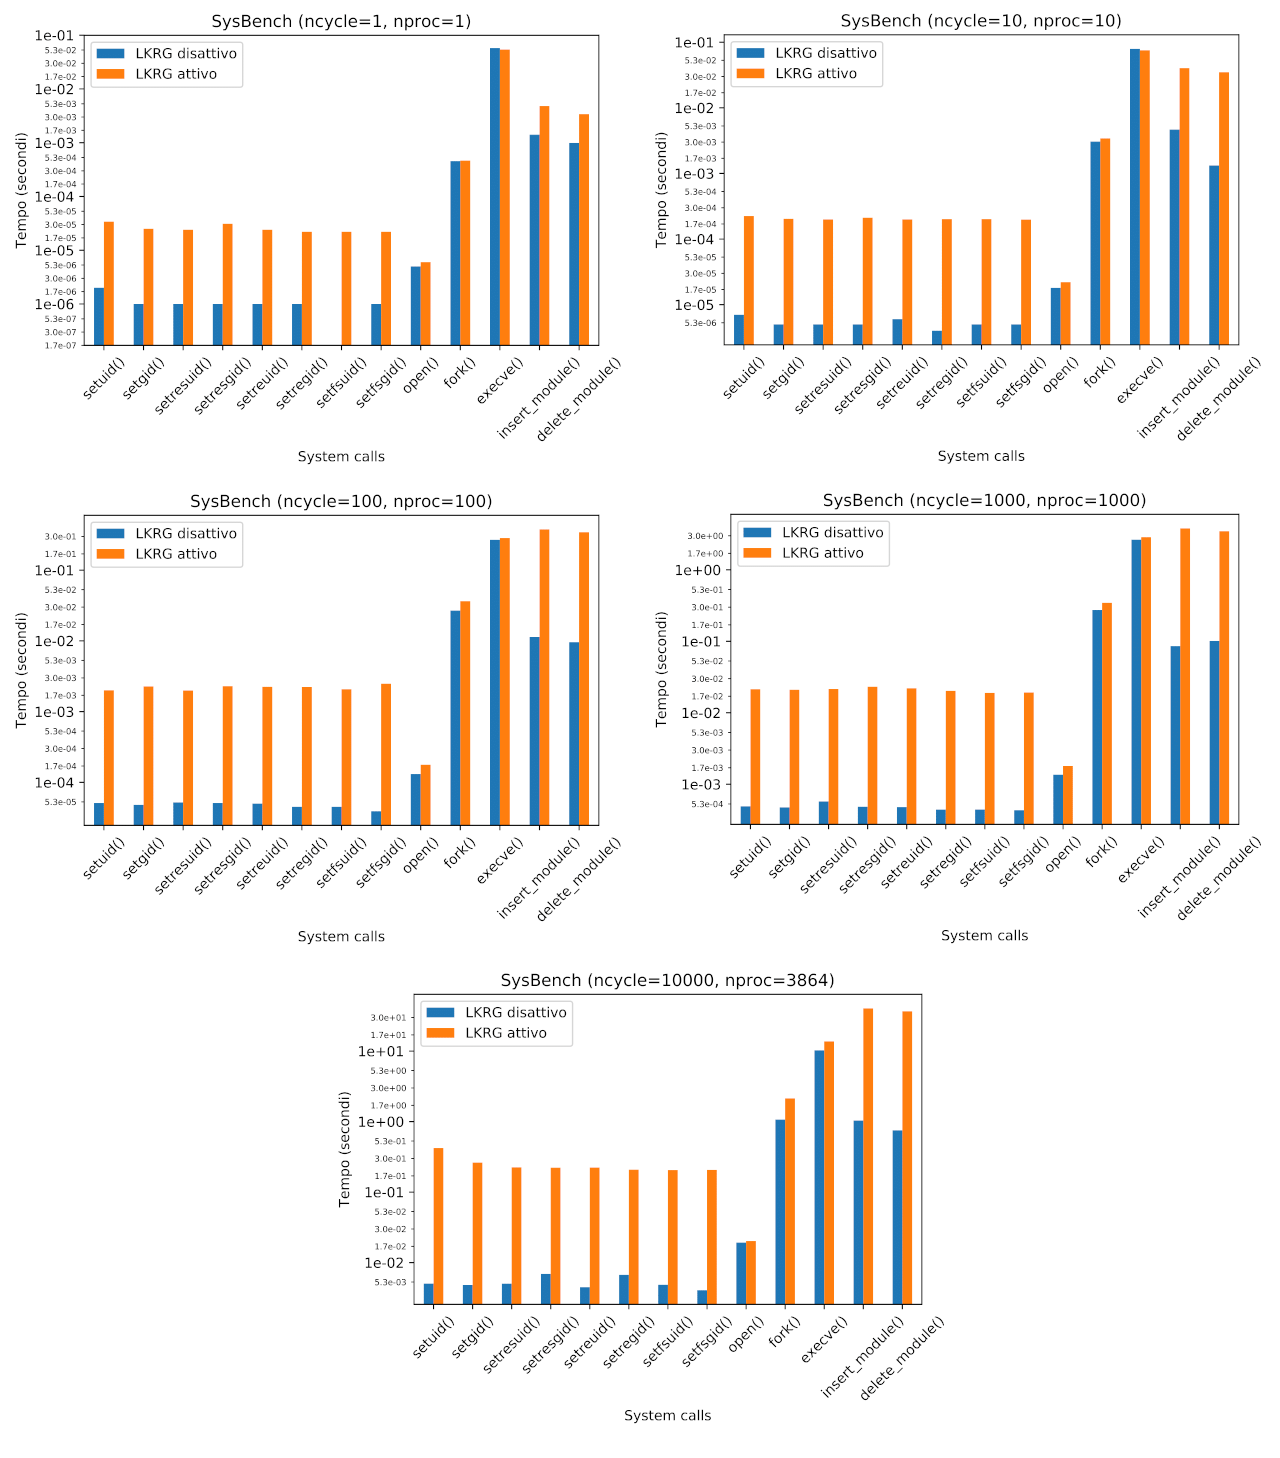
\includegraphics[scale=1.3]{Figures/Mint/Total}
\caption[Benchmark tempo totale (Mint)]{Benchmark tempo totale (Mint).}
\label{fig:totMintFig}
\end{figure}

La \emph{open()}, \emph{execve()} e la \emph{fork()} risultano ancora una volta essere le system call meno influenzate, i cui tempi d'esecuzione variano talmente poco che durante il test è quasi impercettibile la differenza (un paio di secondi in più per la execve quando il modulo è attivo e ncycle=10000). I tempi in relazione al loro ordine di grandezza ottenuti in seguito al test della \emph{insert\_module()} e \emph{delete\_module()} sono i più elevati, per cui la differenza lanciando un programma che esegue tali funzionalità diventa tanto più evidente quanto incrementa il numero di volte che vengono invocate: ad esempio considerando la prima delle due, la quale presenta una differenza pari a $3x10^{-3}$ tra le due esecuzioni e lanciando il test in cui tale system call viene invocata 10000 volte, il tempo d'esecuzione, non considerando le ottimizzazioni, aumenterebbe di $3x10^{1}$ volte, ovvero 30 secondi.

Nella \autoref{table:totMintData} sono riportati i dati di tutte le system call relativi a quest'ultimo test. Si osservi nuovamente che questi dati si discostano parecchio da quelli contenuti nella \autoref{table:setxMintData} e \autoref{table:othersMintData}, come era già successo nei casi precedenti. Vi è persino una differenza di $10^{2}$ tra il valore medio della singola esecuzione di \emph{insert\_module()} presentato in questa tabella e quello in \autoref{table:othersMintData}. Perciò è corretto assumere che vi sia stato un intervento di ottimizzazione, come si può osservare nei grafici sottostanti.

Anche in questo sistema è risultato che il tempo medio della singola system call ad esclusione della \emph{setfsuid()} diminuisce in base al numero di volte che viene richiamata. Nei grafici successivi è possibile osservare come il tempo d'esecuzione delle chiamate quando LKRG non è caricato risulta essere massimo nel test con ncycle=1, mentre raggiunge il minimo valore registrato nel test con ncycle=10000. In presenza del modulo, il tempo di tali funzionalità è molto variabile, talvolta esponenziale come nel grafico della \emph{execve()} in \autoref{fig:mean3MintFig}, mentre altre volte raggiunge dei picchi di massimo e minimo per poi variare nuovamente (si veda la \emph{fork()} o la \emph{setfsuid()}).

Si ricorda che per questi ultimi grafici è stata utilizzata una scala logaritmica per l'asse delle x, in modo tale da rappresentare i valori esponenziali assunti da ncycle.

\begin{figure}[!htbp]
\centering
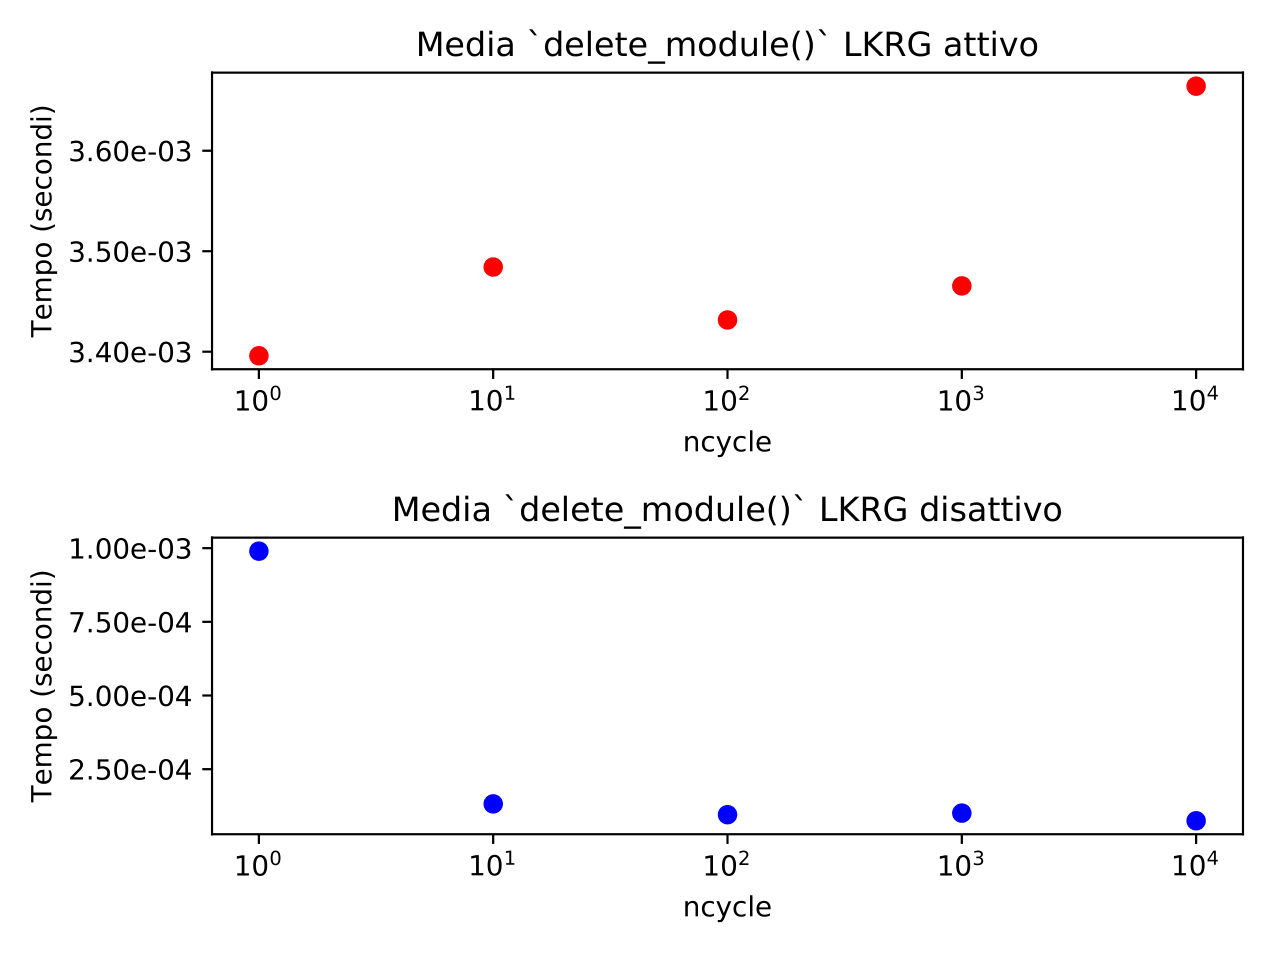
\includegraphics[scale=0.25]{Figures/Mint/Mean1}
\caption[Media singole system call nei 5 benchmark parte 1 (Mint)]{Media singole system call nei 5 benchmark parte 1 (Mint).}
\label{fig:mean1MintFig}
\end{figure}

\begin{figure}[!htbp]
\centering
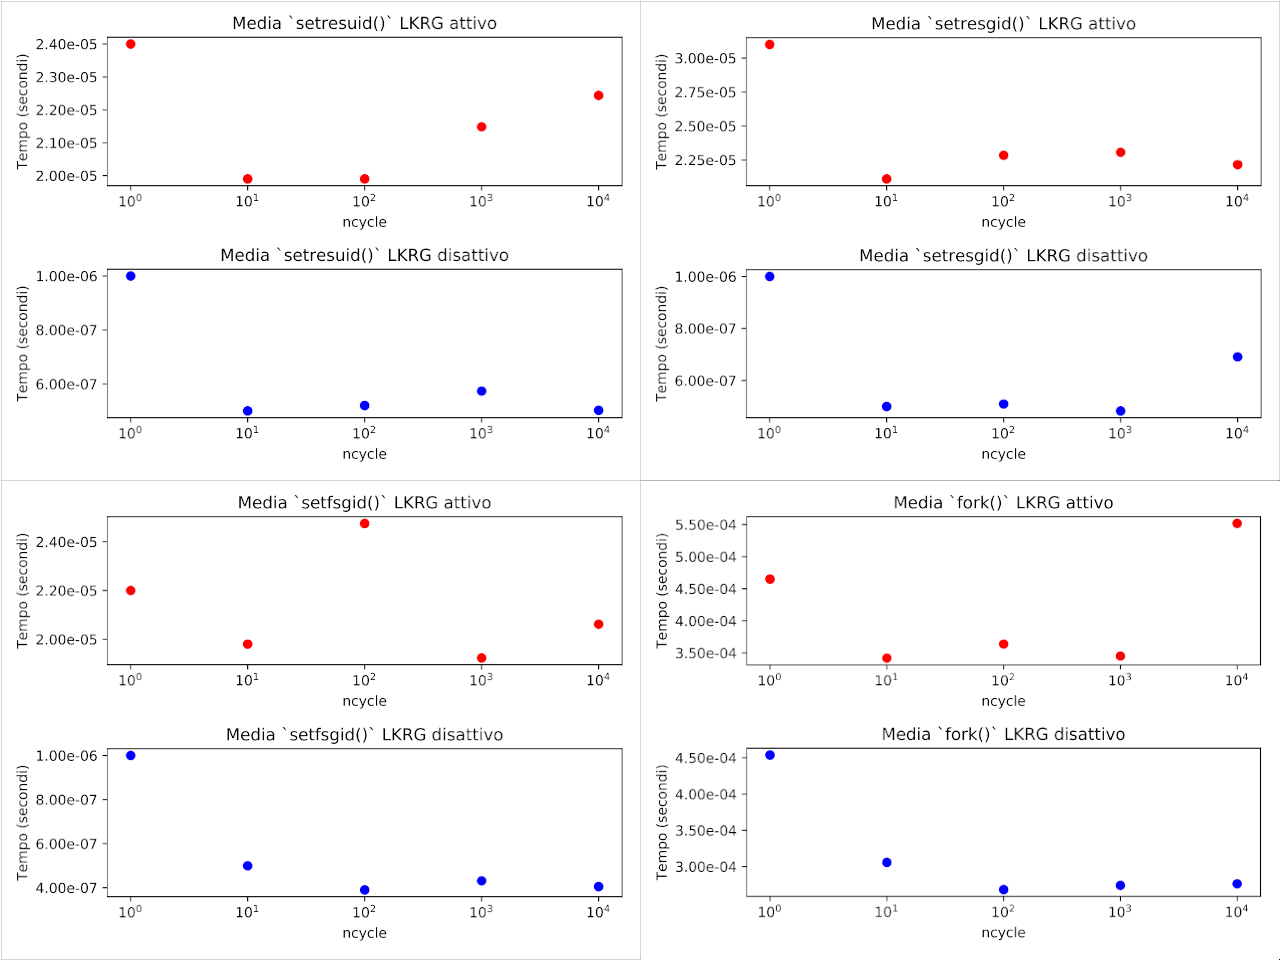
\includegraphics[scale=1.35]{Figures/Mint/Mean2}
\caption[Media singole system call nei 5 benchmark parte 2 (Mint)]{Media singole system call nei 5 benchmark parte 2 (Mint).}
\label{fig:mean2MintFig}
\end{figure}

\begin{figure}[!htbp]
\centering
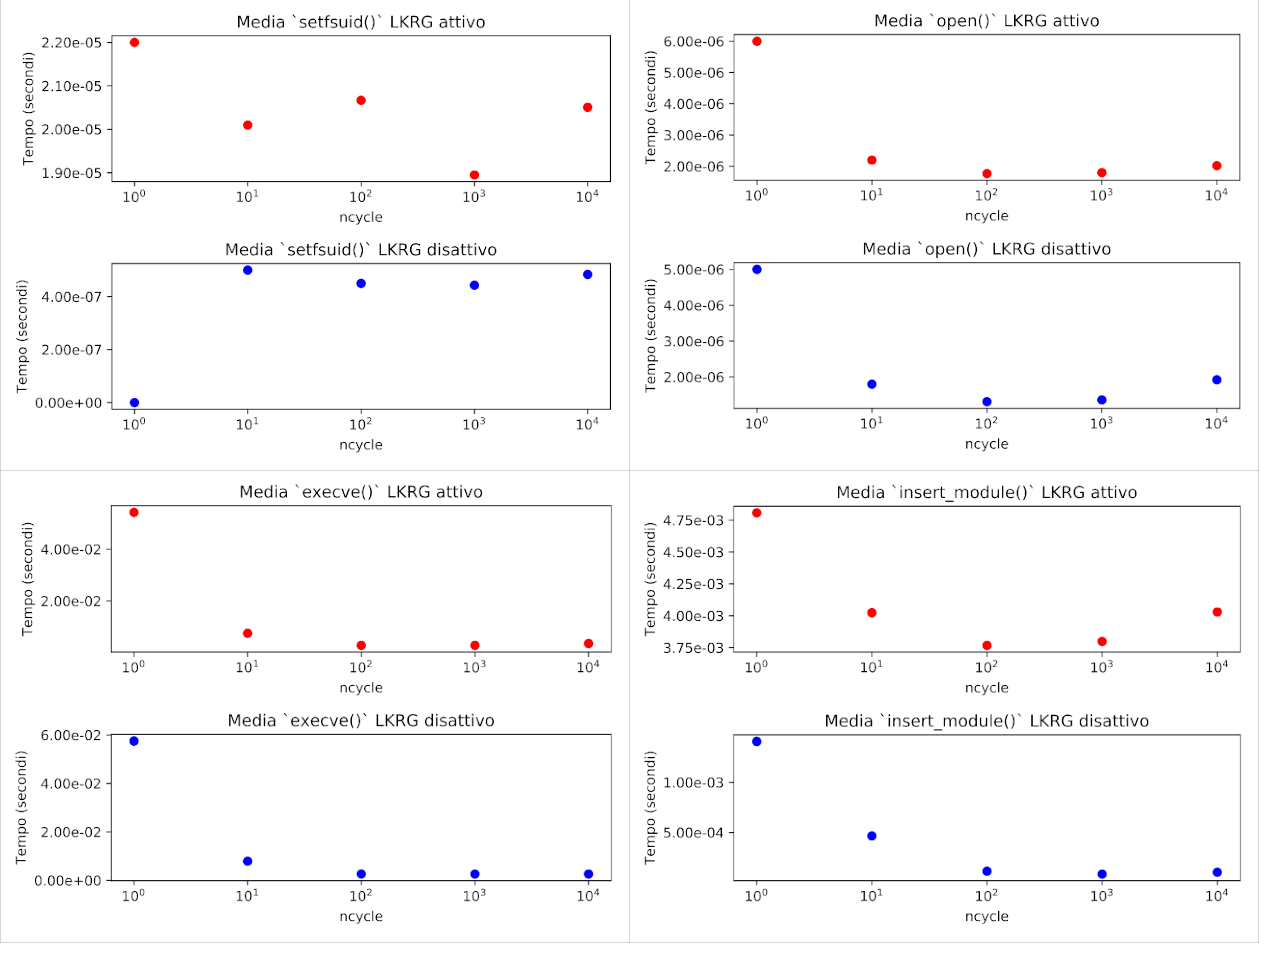
\includegraphics[scale=1.35]{Figures/Mint/Mean3}
\caption[Media singole system call nei 5 benchmark parte 3 (Mint)]{Media singole system call nei 5 benchmark parte 3 (Mint).}
\label{fig:mean3MintFig}
\end{figure}

\begin{figure}[!htbp]
\centering
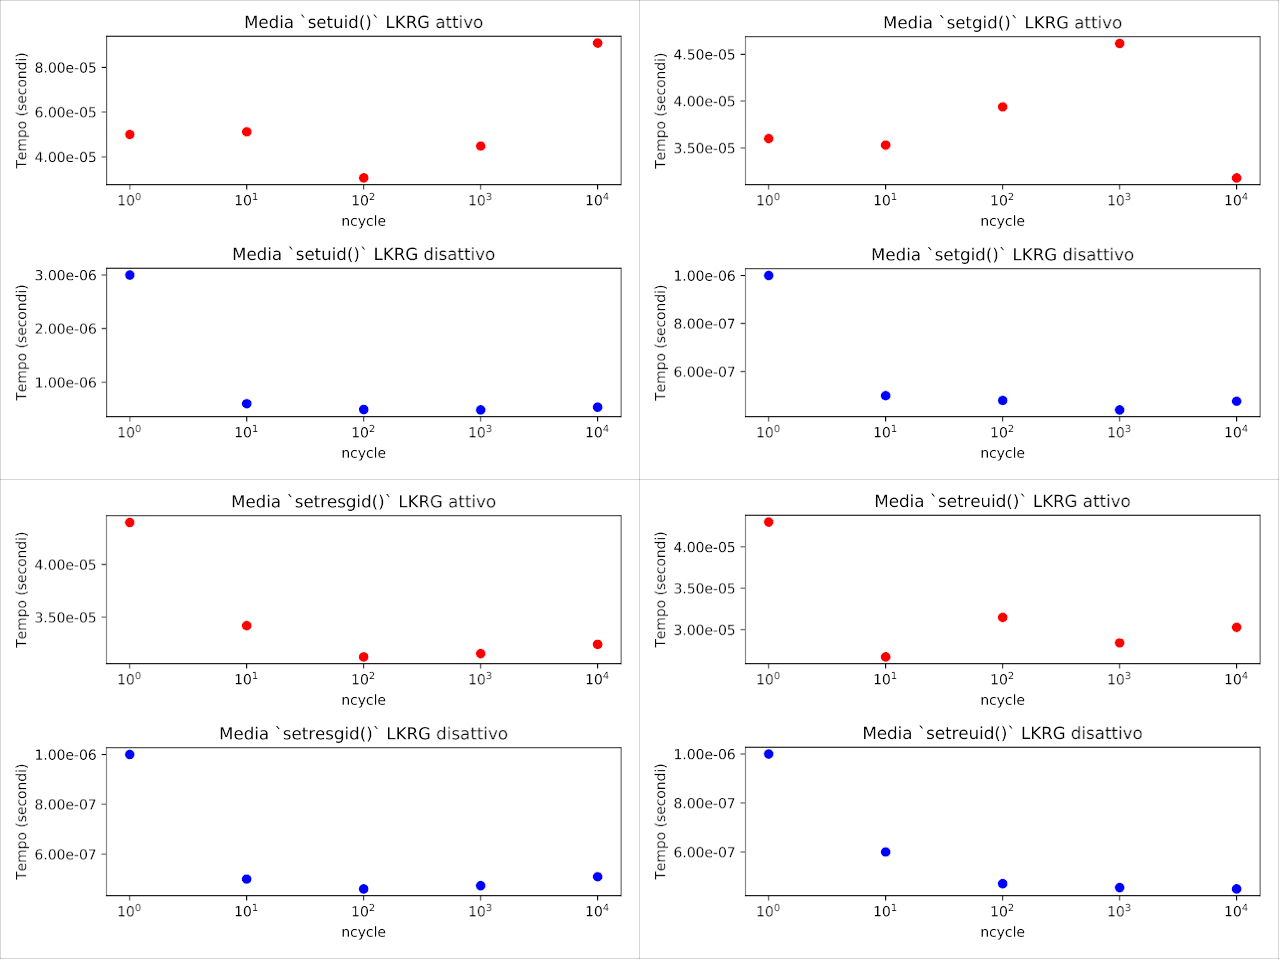
\includegraphics[scale=1.35]{Figures/Debian/Mean4}
\caption[Media singole system call nei 5 benchmark parte 4 (Mint)]{Media singole system call nei 5 benchmark parte 4 (Mint).}
\label{fig:mean4MintFig}
\end{figure}

%----------------------------------------------------------------------------------------
%	COMPARISON
%----------------------------------------------------------------------------------------
\section{I tre sistemi a confronto}

Nel corso della trattazione dei test nei vari sistemi sono già state anticipate alcune somiglianze e differenze dei risultati. In questa sezione conclusiva l'attenzione è rivolta all'aumento percentuale del tempo d'esecuzione delle system call in seguito al caricamento di \emph{Linux Kernel Runtime Guardian}, commentando appropriatamente i valori ottenuti. Per ottenere in formule matematiche il tempo misurato con LKRG presente, bisogna attenersi alla legge:\\
$T_f = T_i + x\%T_i => T_f = T_i * (1 + x\%)$

Ad esempio se una chiamata presenta un aumento pari al 100\%, il tempo finale è $T_f = T_i * (1 + 100\%) = T_i * 2 = 2T_i$, ovvero il doppio.

\begin{table}[!htbp]
\centering
\begin{tabular}{|c|c|c|c|c|}
\hline
\textbf{SystemCall} & \bm{$\Delta$}\textbf{ Ubuntu (\%)} & \bm{$\Delta$}\textbf{ Debian (\%)} & \bm{$\Delta$}\textbf{ Mint (\%)} \\
\hline
setuid() & 2332 & 2193 & 1875 \\
\hline
setgid() & 213 & 102 & 121 \\
\hline
setresuid() & 3659 & 735 & 2328 \\
\hline
setresgid() & 296 & 1597 & 365 \\
\hline
setreuid() & 3144 & 1478 & 2136 \\
\hline
setregid() & 283 & 884 & 327 \\
\hline
setfsuid() & 3406 & 1519 & 3347 \\
\hline
setfsgid() & 3824 & 1861 & 4746 \\
\hline
open() & 3089 & 1978 & 3051 \\
\hline
fork() & 2792 & 1906 & 3043 \\
\hline
execve() & 123 & 143 & 115 \\
\hline
insert\_module() & 137 & 75 & 84 \\
\hline
delete\_module() & 3432 & 1411 & 3581 \\
\hline
\hline
Media & 2056 & 1222 & 1932 \\
\hline
\end{tabular}
\caption{Aumento percentuale tempo d'esecuzione nei 3 sistemi}
\label{table:compareData}
\end{table}

Dalla \autoref{table:compareData} si evince che le system call minormente influenzate dal modulo in tutti i sistemi sono la \emph{setuid()}, \emph{setregid()}, \emph{execve()} e \emph{insert\_module()}, in quanto il tempo d'esecuzione a causa dei controlli d'integrità raddoppia o triplica al massimo. Al contrario, le rimanenti funzioni subiscono un aumento rilevante che varia dal 800\% per la \emph{setregid()} (corrispondente a 9 volte il tempo iniziale) ad un massimo di 4746 per la \emph{setfsgid()}, ovvero poco più di $48T_i$.

Questi elevati valori porterebbero a pensare che LKRG rallenti pesantemente il sistema nel quale è installato, portando sfortunatamente alla conclusione sbagliata. Quando si osservano delle percentuali bisogna sempre fare riferimento ai tempi di partenza e al loro ordine di grandezza: ad esempio, un aumento del 100\% in una chiamata che impiega 1 secondo ad essere soddisfatta è più rilevante di un aumento pari a 5000\% di una system call il cui tempo d'esecuzione è dell'ordine di $10^{-7}$. Per questi motivi, dopo aver analizzato tutti i grafici ed i tempi riportati in questo capitolo, è possibile farsi un'idea circa l'effettivo overhead del sistema, riferendosi ad un caso d'uso personale.

Dai grafici e dai dati è risultato che sicuramente in tutti e tre i sistemi LKRG effettua i controlli con tempi differenti, nonostante l'installazione ed l'esecuzione di SysBench fosse avvenuta nelle medesime condizioni. L'ultima riga della tabella riporta l'incremento percentuale medio delle system call in ogni sistema; si osservi come in base a questi valori il sistema al quale LKRG aggiunge maggiore overhead risulti essere Ubuntu, seguito da Mint ed infine Debian.

Dovendo prestare attenzione ad un possibile scenario reale, si pensi ad un server hostato in un sistema Ubuntu, dal quale in base ad alcune richieste dell'utente vengono lanciati i comandi \emph{execve()}, \emph{fork()} e \emph{open()}. Essendo i tre maggiormente utilizzati si vuole valutare se vale la pena o meno inserire LKRG nel server, per evitare che il tempo di risposta del server renda l'esperienza utente meno gradevole. Dall'analisi è risultato che l'aumento in percentuale delle funzioni è rispettivamente pari a 123\%, 2792\% e 3089\%. Per cui assumento come tempi per ogni singola chiamata i valori riportati nella tabella \autoref{table:othersUbuntuData}, ovvero $7.74x10^{-6}, 3.518x10^{-5}$ e $3.398x10^{-5}$ ed ipotizzando che per ogni utente vengono gestite singolarmente mille istanze delle seguenti operazioni (ncycle=1 ntimes=1000, esecuzione di SysBench tramite lo script), si ha che:\\\\
$TempoFinale_{execve} = 7.74x10^{-6} * (1 + 1.23) * 1000 = 0.01726$ secondi\\
$TempoFinale_{fork} = 3.518x10^{-5} * (1 + 27.92) * 1000 = 1.01741$ secondi\\
$TempoFinale_{open} = 3.398x10^{-5} * (1 + 30.89) * 1000 = 1.0836222$ secondi
\\\par

Nonostante questo scenario sia estremo, in quanto non accadrà mai di gestire 1000 di queste system call per un singolo utente, si ha che la richiesta verrà soddisfatta nei tempi riportati, i quali sono estremamente bassi. Si pensi infatti se l'esperienza utente è veramente influenzata da un ritardo di 1 secondo in una risposta; sono tempi molto piccoli, difficile da percepire se non effettuandone una valutazione con un programma come SysBench.
\addchap{Conclusioni}

\label{Chapter5}

In un mondo in cui proteggere le informazioni è diventato oramai un obiettivo di vitale importanza è necessario essere consapevoli dell'esistenza di software in grado di aumentare l'integrità e la sicurezza del proprio sistema. Bisogna però tener conto del trade-off sicurezza-tempo, due importanti fattori talvolta antagonisti, in quanto più si aggiungono layer protettivi al sistema, più aumenta il tempo di risposta. È necessario valutare attentamente le proprie necessità prima di installare qualsiasi materiale, decidendo quali sono e come si possono raggiungere gli obiettivi prestabiliti, valutando se si preferisce garantire un'ottima prontezza di risposta, o la sicurezza (e non è detto che non vi sia un modo per oltrepassare queste ulteriori difese), oppure se raggiungere una soluzione intermedia ricoprendo entrambe le qualità.

Pertanto, in seguito all'analisi sviluppata in questo elaborato, è vivamente consigliato l'uso del modulo \emph{Linux Kernel Runtime Guardian}, il quale non solo è sorprendentemente performante, ma garantisce anche l'integrità dei dati e rileva efficacemente molte minacce al sistema che comprometterebbero la sua sicurezza. Nelle macchine testate, nonostante fossero ambienti virtuali e non fisici, si sono ottenuti ottimi risultati che portano a valutarne positivamente l'uso non solo nella propria installazione locale, ma anche nei vari server utilizzati con obiettivi differenti. Infatti, si è valutato l'utilizzo di LKRG anche in calcolatori con installazioni di Linux meno recenti (ad esempio negli ATM), le quali per problemi di supporto non vengono aggiornate, non curandosi in questo modo di possibili nuovi vettori d'attacco che si sono sviluppati negli ultimi anni. Con un trascurabile calo delle performance, il modulo potrebbe offrire a questi sistemi un maggior livello di sicurezza, favorendone il continuo utilizzo.

Infine, un ulteriore aspetto ritenuto personalmente importante è l'utilizzo di software libero: rispetto ad uno definito "proprietario", la cui licenza non ne permette la modifica, lo studio, la ridistribuzione e la condivisione tenendo segreto il sorgente (l'utente è limitato al semplice utilizzo), un software pubblicato sotto i termini di una licenza di software libero concede lo studio, la modifica e la ridistribuzione del progetto stesso. In questo modo non solo l'utente è a conoscenza della struttura del software potendosi leggere il sorgente, ma può anche apportare dei miglioramenti e condividerli con il resto della community. È grazie a questa filosofia che il mondo Linux è attraente ed efficace, in quanto offre la possibilità di costruire gratuitamente e liberamente il proprio sistema senza avere vincoli nei confronti di nessuno. 

In conclusione, LKRG offre un servizio a dir poco eccezionale, facendo sì che anche l'utente meno esperto e senza disponibilità economiche possa difendersi da certi tipi di minacce in maniera semplice ed efficace subendo una diminuzione accettabile delle performance.



%----------------------------------------------------------------------------------------
%	APPENDIX
%----------------------------------------------------------------------------------------

\setcounter{section}{0}
\renewcommand{\thesection}{A.\arabic{section}}%
% Appendix A

\addchap{Appendice A} % Main appendix title

\label{AppendixA} % For referencing this appendix elsewhere, use \ref{AppendixA}

Per compilare il progetto SysBench e \emph{Linux Kernel Runtime Guardian} sono necessari vari strumenti ottenibili mediante il proprio gestore di pacchetti. Le distribuzioni presentare sfruttano lo stesso comando per scaricare ed installare nuovi pacchetti nel proprio sistema, ovvero \emph{apt}.

Una volta scaricata ed installata a piacere la propria distribuzione, aprire il terminale e tramite il comando \emph{sudo apt install} (nel nostro caso) installare:

\begin{itemize}
\item linux-headers-\$(uname -r), necessario al fine della compilazione del kernel e la build dei moduli (\$(uname -r) viene sostituito dalla versione attuale del proprio kernel, al fine di ottenere i giusti headers);
\item build-essential, comprende il compilatore gcc e make, necessari per la compilazione dei software;
\item libelf-dev, per la lettura e scrittura dei file ELF (eseguibili) ad alto livello.
\end{itemize}

A questo punto il sistema è configurato per la compilazione corretta dei due software.

\section{Installazione del \emph{Linux Kernel Runtime Guardian}}

Per installare LKRG nel proprio sistema è necessario seguire le seguenti istruzioni:\\\\
1.Scaricare LKRG al seguente link ufficiale \url{https://www.openwall.com/lkrg/}. \\
2.Accedere tramite terminale alla directory in cui si trova: \emph{cd path\_to\_dir}.\\
3.Estrarre il contenuto del file .zip: \emph{tar -xzvf lkrg-0.4.tar.zip}.\\
4.Entrare nella cartella creata: \emph{cd lkrg-0.4}.\\
5.Compilare il progetto: \emph{make -j8}\\
6.Entrare nella cartella di output: \emph{cd output}\\
7.Caricare la versione .ko ottenuta in seguito alla compilazione del modulo: \emph{sudo insmod output/p\_lkrg.ko p\_init\_log\_level=3}, dove \emph{p\_init\_log\_level} è il parametro in ingresso tramite il quale si decide il livello di logging delle informazioni in console (e non nel terminale, bensì nell'esecuzione del proprio sistema in modalità console e non desktop, accedendovi premendo CTRL+ALT+F7).\\
8.Controllare che LKRG sia stato effettivamente caricato: \emph{lsmod | grep p\_lkrg}.\\

Per rimuoverlo dal kernel è sufficiente utilizzare \emph{sudo rmmod p\_lkrg} e controllare che sia stato rimosso.

In caso vi fossero problemi con la compilazione del modulo, contattare l'autore tramite la mailing list presente nel sito indicato precedentemente.

\section{Installazione di \emph{SysBench}}

Il procedimento per installare SysBench è il seguente:\\\\
1.Accedere al mio repository online tramite browser e copiare l'indirizzo fornito cliccando il tasto \emph{clone}.\\
2.Clonare il repository nel proprio computer digitando da terminale: \emph{git clone https://SimoMagno@bitbucket.org/SimoMagno/sysbench.git}.\\
3.Accedere alla cartella clonata: \emph{cd sysbench}.\\
4.Compilare il progetto: \emph{make}.

A questo punto il progetto è eseguibile e si può lanciare in due maniere presentate:

\begin{itemize}
\item singola esecuzione : \emph{[sudo] ./sysbench ncycle filename};
\item multipla esecuzione: \emph{sudo ./script.sh ntimes ncycle path/to/p\_lkrg.ko}
\end{itemize}

Il primo scenario è il normale caso di esecuzione di programma da riga di comando, in cui viene richiamato passando i parametri \emph{ncycle} (intero) e \emph{filename} (stringa); viene eseguito un singolo benchmark in cui ogni system call viene chiamata ncycle-volte ed il risultato è salvato nel file indicato. Da notare che in questo il programma può essere eseguito sia con i privilegi sia senza, in quanto la parte di caricamento/rimozione del modulo LKRG nel kernel è stata volutamente lasciata a carico dell'utente.

Nel secondo caso, il programma viene lanciato ntimes-volte producento altrettanto file di output, ognuna delle quali effettua il test delle system call invocate ncycle-volte. La differenza sostanziale consiste nel tempo d'esecuzione medio e totale delle chiamate a funzione: si è osservato infatti che per valutare il tempo medio d'esecuzione di una system call è più preciso effettuare ntimes-volte il benchmark con parametro ncycle=1, in quanto se la stessa funzione è richiamata più volte all'interno dello stesso programma possono esserci dei salvataggi in cache e miglioramenti apportati dalla glibc, dalla cache o dal processore, i quali alterano i risultati come mostrato nel Capitolo 4. Per questa tipologia d'esecuzione sono necessari i privilegi di root, in quanto il caricamento e rimozione di LKRG è a carico dello script ogni volta che SysBench viene eseguito.

Per qualsiasi tipo di informazione o chiarimento sentitevi liberi di contattarmi.


%----------------------------------------------------------------------------------------
%	ACKNOWLEDGEMENTS
%----------------------------------------------------------------------------------------

\begin{acknowledgements}
\addchaptertocentry{\acknowledgementname} % Add the acknowledgements to the table of contents

Grazie a tutti coloro che mi hanno costantemente supportato lungo questo ricco percorso di studio. In particolare il pensiero è rivolto:

ai miei genitori Fabrizio e Rosanna, per avere sostenuto economicamente quest'esperienza;

a mio fratello Francesco, per avermi sopportato in casa e per la sua ispiratrice determinazione e perseveranza nel raggiungere gli obiettivi;

alla mia ragazza Catarina, perchè è stata e continua ad essere una compagna di viaggio impeccabile, disponibile e motivatrice;

ai miei cari amici, per il loro sostegno, la loro presenza e i loro scherzi i quali hanno reso le giornate di studio meno pesanti e il tempo libero ancora più prezioso;

al team di CeSeNA Security, per avermi fatto scoprire il vastissimo mondo della sicurezza informatica ed avermi guidato in questa realtà a me fino ad ora sconosciuta;

al mio relatore prof. Gabriele D'Angelo, per le sue lezioni essenziali e appassionanti, le quali hanno sicuramente influenzato la mia scelta di fare della sicurezza informatica il mio interesse di studio.
\\\par
Ho incluso brevemente tutte le persone rilevanti con le quali spero di rimanere sempre in contatto, perchè ognuno a modo suo ha avuto (e spero continui ad avere) un ruolo determinante nella mia crescita.

\end{acknowledgements}


%----------------------------------------------------------------------------------------
%	BIBLIOGRAPHY
%----------------------------------------------------------------------------------------

\printbibliography[heading=bibintoc]

%----------------------------------------------------------------------------------------

\end{document}  
